\phantomsection
\addcontentsline{toc}{section}{Εισαγωγή - σκοπός}
\section*{Εισαγωγή και σκοπός}
Στις σύγχρονες αγωνιστικές διοργανώσεις, τα ελαστικά αποτελούν ίσως τον πιο καθοριστικό 
παράγοντα επίδοσης και στρατηγικής. Τα ελαστικά λειτουργούν εντός ενός
στενού παραθύρου θερμοκρασίας (\textit{thermal window}): κάτω από ένα κατώτατο όριο η σύνθεση του
υλικού δεν μπορεί να αποδώσει τη μέγιστη πρόσφυση, ενώ πάνω από ένα ανώτατο η αυξημένη
θερμοκρασία επιταχύνει τη φθορά του πέλματος και μειώνει την πρόσφυση. Η κατανόηση και η ακριβής
μοντελοποίηση αυτής της συμπεριφοράς έχει τεράστια πρακτική αξία τόσο για τη
βελτιστοποίηση της απόδοσης ανά γύρο όσο και για τον σχεδιασμό της στρατηγικής του αγώνα, καθώς η φθορά του πέλματος αποτελεί τον πρωταρχικό παράγοντα που ορίζει τη στρατηγική
αντικατάστασης ελαστικών (\textit{pit-stop strategy}). Κάθε τύπος ελαστικού παρουσιάζει διαφορετική 
ισορροπία μεταξύ επίδοσης και
ανθεκτικότητας, και η βέλτιστη επιλογή εξαρτάται από χαρακτηριστικά πίστας, συνθήκες αγώνα
και τη συμπεριφορά οδήγησης \cite{West2022, Tremlett2016}. Η ακριβής πρόβλεψη του ρυθμού φθοράς
για δεδομένο προφίλ οδήγησης είναι εξαιρετικά δύσκολη και συνεχίζει να αποτελεί
αντικείμενο έρευνας.

Οι προσομοιωτές χρόνου γύρου (lap time simulators) αποτελούν βασικό εργαλείο στην ανάπτυξη
αγωνιστικών οχημάτων. Η πλειονότητά τους βασίζεται στην προσέγγιση ψευδο-μόνιμης κατάστασης
(\textit{Quasi-Steady-State -- QSS}), η οποία χρησιμοποιεί ένα διάγραμμα επιδόσεων (GGV
diagram) ως στατική χαρτογράφηση των δυνατοτήτων του οχήματος σε κάθε ταχύτητα. Η
χαρτογράφηση αυτή κατασκευάζεται συνήθως για σταθερές, ιδανικές συνθήκες ελαστικού --
σταθερή θερμοκρασία και μηδενική φθορά -- αγνοώντας τη δυναμική εξέλιξη της κατάστασης των
ελαστικών κατά τη διάρκεια του αγώνα.

Με βάση τις ανάγκες της σύγχρονης μορφής του μηχανοκίνητου αθλητισμού, η παραδοχή αυτή
αγνοεί μεγάλο μέρος των συνθηκών λειτουργίας του οχήματος κατά τη διάρκεια ενός αγώνα και, λόγω της ευαισθησίας των ελαστικών,
εισάγει σημαντικό σφάλμα στα σενάρια όπου η κατάστασή τους
αποκλίνει από την ιδανική: κατά τους πρώτους γύρους προθέρμανσης (out-lap), σε συνθήκες υψηλής φόρτισης
που οδηγούν σε υπερθέρμανση, ή κοντά στο τέλος της ζωής των ελαστικών. Επομένως, η πρόβλεψη χρόνου γύρου χωρίς να λαμβάνεται υπόψη η θερμοκρασία των ελαστικών
αφενός μπορεί να διαφέρει σημαντικά από την πραγματικότητα, αλλά σημαντικότερα δεν επιτρέπει την 
ανάλυση της στρατηγικής ενός αγώνα προκαταβολικά ή σε πραγματικό χρόνο.

Στη βιβλιογραφία υπάρχει καταγεγραμμένη έρευνα τα τελευταία χρόνια για την ανάπτυξη μοντέλων πρόβλεψης 
θερμοκρασίας και φθοράς -- είτε απλούστερα είτε πιο λεπτομερή όπου στην πλειοψηφία τους
χρησιμοποιούν μη-μόνιμους προσομοιωτές χρόνου γύρου (\textit{Transient lap time simulators}). Οι μη-μόνιμοι προσομοιωτές είναι συνήθως ακριβέστεροι έναντι των προσομοιωτών ψευδο-μόνιμης κατάστασης, ωστόσο, μπορεί να εισάγουν αβεβαιότητα
λόγω της ανάγκης τους για μοντέλο οδηγού, και επίσης είναι πιο ασταθείς και υπολογιστικά κοστοβόροι. Οι προσομοιωτές ψευδο-μόνιμης κατάστασης χρησιμοποιούνται
κυρίως σε μελέτες αρχιτεκτονικής του οχήματος όπου απαιτείται η χαρτογράφηση των μέγιστων δυνατών επιδόσεων του οχήματος.

\subsection*{Σκοπός και συνεισφορά}

Ο σκοπός της παρούσας διπλωματικής εργασίας είναι η ανάπτυξη ενός υπολογιστικού πλαισίου προσομοίωσης χρόνου γύρου ψευδο-μόνιμης κατάστασης λαμβάνοντας υπόψη
την επίδραση της θερμοκρασίας και της φθοράς. Συγκεκριμένα, αναπτύσσεται ένα 
μοντέλο που μοντελοποιεί τη
θερμοκρασία και τη φθορά των ελαστικών κατά τη διάρκεια ενός γύρου, και ενσωματώνει αυτή
τη δυναμική στον υπολογισμό του διαγράμματος επιδόσεων - GGV. Επιλέγεται η ανάπτυξη ενός φυσικού θερμοδυναμικού μοντέλου έναντι άλλων 
(όπως για παράδειγμα μοντέλου μηχανικής μάθησης \cite{Todd_2025}) αφενός γιατί επιτρέπει την κατανόηση των μηχανισμών των φαινομένων που λαμβάνουν χώρα και
αφετέρου, μετά την επαλήθευση του μοντέλου, μπορεί εύκολα να γενικευθεί σε περισσότερους συνδυασμούς οχήματος--ελαστικών--πίστας.
Το αποτέλεσμα του μοντέλου είναι ένα
\emph{χρονο-μεταβαλλόμενο} διάγραμμα GGV που αντικατοπτρίζει τη στιγμιαία κατάσταση των ελαστικών,
και συνδέεται με τον προσομοιωτή QSS ανοιχτού κώδικα \openLap για την εκτίμηση χρόνου γύρου.\\[8pt]

\noindent
Η κύρια συνεισφορά της εργασίας συνοψίζεται:
\begin{enumerate}
    \item Ανάπτυξη φυσικού θερμικού μοντέλου ελαστικού.
    \item Μοντελοποίηση τριών ανεξάρτητων μηχανισμών φθοράς.
    \item Σύνδεση θερμοκρασίας--φθοράς με την πρόσφυση για τη δυναμική ανανέωση του GGV.
    \item Διαδικασία υπολογισμού θερμοκρασίας: χρησιμοποιώντας δεδομένα πίστας/ταχύτητας από προσομοίωση ή πειραματικά δεδομένα 
    (εφαρμογή στην πίστα της Βαρκελώνης -- Circuit de Barcelona-Catalunya) 
    \item Προσομοίωση χρόνου γύρου λαμβάνοντας υπόψη τη θερμοκρασία και φθορά των ελαστικών
    \item Μελέτη διατήρησης ελαστικών -- συσχέτιση χρόνου γύρου με συνολική φθορά% [TODO]
\end{enumerate}

\subsection*{Δομή εργασίας}

Στη συνέχεια, το κεφάλαιο \ref{sec:tyre_theory} ξεκινά παρουσιάζοντας τη θεωρητική βάση για τη
συμπεριφορά ελαστικών: μηχανισμούς παραγωγής θερμότητας, απαγωγής και φθοράς. Το
κεφάλαιο \ref{sec:tyre_model} αναπτύσσει τα υπολογιστικά μοντέλα πρόσφυσης, θερμότητας και
φθοράς με βάση τη θεωρία που παρουσιάστηκε. Έπειτα, το κεφάλαιο \ref{sec:vehicle_model} περιγράφει
το μαθηματικό μοντέλο του οχήματος. Το κεφάλαιο \ref{sec:inverseModel} παρουσιάζει τη μέθοδο εκτίμησης
της κατάστασης του οχήματος -- μεγέθη ολίσθησης και φορτία τροχών -- από το προφίλ ταχύτητας και τη
γεωμετρία της πίστας, ενώ το κεφάλαιο \ref{sec:parameterFitting} περιγράφει τη διαδικασία βαθμονόμησης
του θερμοδυναμικού μοντέλου από πειραματικά δεδομένα. Στο κεφάλαιο \ref{sec:lapSim} αναλύεται η
κατασκευή του διαγράμματος επιδόσεων και η ενσωμάτωσή του στον προσομοιωτή \openLap, και στο
κεφάλαιο \ref{sec:results} παρουσιάζονται τα αποτελέσματα για ένα όχημα τύπου \textit{Formula 1} στην
πίστα \textit{Circuit de Barcelona-Catalunya}. Τέλος, στο κεφάλαιο \ref{sec:conclusions} συνοψίζονται
τα συμπεράσματα, οι περιορισμοί του μοντέλου και οι προτάσεις για μελλοντικές βελτιώσεις.

\clearoddpage
\section{Βασικά στοιχεία θεωρίας ελαστικών}
\label{sec:tyre_theory}
\subsection{Βασική θεωρία ελαστικού}
\subsubsection{Ανάπτυξη δυνάμεων στο ελαστικό}
Το ελαστικό αποτελεί το βασικό μηχανικό στοιχείο μέσω του οποίου το
όχημα αλληλεπιδρά με το οδόστρωμα. Μέσω της περιοχής επαφής
μεταφέρονται στο όχημα η κατακόρυφη δύναμη, η διαμήκης δύναμη και η
πλευρική δύναμη. Το πέλμα του ελαστικού (η επιφάνεια επαφής με το οδόστρωμα) 
δεν είναι σταθερό, αλλά επηρεάζεται από το κατακόρυφο φορτίο, την πίεση, 
τη γωνία κάμπερ και τη γεωμετρία του ελαστικού \cite{Pacejka2012,Farroni2014TRT}.


Η διαμήκης δύναμη $F_x$ σχετίζεται με την πέδηση και την
επιτάχυνση. Αναπτύσσεται όταν υπάρχει διαφορά μεταξύ της περιφερειακής
ταχύτητας του ελαστικού και της ταχύτητας με την οποία μετακινείται το
κέντρο του τροχού. Η διαφορά αυτή περιγράφεται μέσω του συντελεστή
διαμήκους ολίσθησης $\kappa$. Συνέπεια αυτού του μηχανισμού είναι πως 
κατά την επιτάχυνση, η περιφερειακή
ταχύτητα του τροχού πρέπει να είναι μεγαλύτερη από την ταχύτητα του
οχήματος, ενώ κατά την πέδηση να είναι μικρότερη
\cite{Pacejka2012,Perantoni2014}.

Η πλευρική δύναμη $F_y$ αναπτύσσεται κατά την αλλαγή διεύθυνσης του
οχήματος. Η αντίστοιχη κινηματική ποσότητα είναι η γωνία ολίσθησης
$\alpha$, η οποία εκφράζει τη διαφορά μεταξύ της διεύθυνσης του επιπέδου
του τροχού και της διεύθυνσης της ταχύτητας στο σημείο επαφής. Μη
μηδενική γωνία ολίσθησης προκαλεί πλευρική παραμόρφωση του πέλματος και
συνεπώς ανάπτυξη πλευρικής δύναμης
\cite{Pacejka2012,Perantoni2014}.

% ============================================================
%  Σχήμα: Παραμορφωμένο ελαστικό σε πλαϊνή όψη -- brush model
%  Απαιτεί: tikz + libraries: arrows.meta, decorations.pathreplacing,
%           calc, positioning (φορτωμένα στο main.tex)
% ============================================================
\begin{figure}[htbp]
    \centering
    \begin{tikzpicture}[
        >={Latex[length=2.2mm,width=1.6mm]},
        font=\small
      ]
      % ------------- Geometry -------------
      \def\R{4.0}
      \def\RE{3.7}
      \def\hCP{0.55}
      \def\tilt{0.18}
      \pgfmathsetmacro{\xC}{sqrt(\R*\R - (\RE-\hCP)*(\RE-\hCP))}
      \pgfmathsetmacro{\aR}{-asin((\RE-\hCP)/\R)}
      \pgfmathsetmacro{\aL}{180 - \aR}

      \coordinate (O) at (0,\RE);

      % ------------- Ground line + hatching (skip under the contact zone) -------------
      \draw[thick] (-\xC-3.8, 0) -- (\xC+3.8, 0);
      \pgfmathsetmacro{\xHg}{-\xC-\tilt}
      \pgfmathsetmacro{\xDg}{\xC}
      \foreach \x in {-5.2,-4.7,...,5.2} {
        \pgfmathparse{(\x < \xHg-0.15) || (\x > \xDg+0.15) ? int(1) : int(0)}
        \ifnum\pgfmathresult=1
          \draw[gray] (\x, 0) -- ++(-0.18,-0.28);
        \fi
      }

      % ------------- Tire outline: arc stops at top of bristles (y = hCP) -------------
      \draw[thick] ($ (O) + (\aR:\R) $)
            arc[start angle=\aR, end angle=\aL, radius=\R];
      \draw[thick] (-\xC, \hCP) -- (\xC, \hCP);

      % ------------- Bristles (brush model, braking: bottoms drag LEFT) -------------
      % Sticking region (right, x >= 0): tilt grows linearly from 0 at x=xC to \tilt at x=0
      % Sliding region  (left,  x < 0):  tilt fixed at \tilt (max deflection)
      \foreach \x in {0.0, 0.2, 0.4, ..., 2.6} {
        \pgfmathsetmacro{\loc}{\tilt * (1 - \x/\xC)}
        \draw[thin] (\x, \hCP) -- ++(-\loc, -\hCP);
      }
      \foreach \x in {-0.2, -0.4, -0.6, ..., -2.6} {
        \draw[thin] (\x, \hCP) -- ++(-\tilt, -\hCP);
      }

      % ------------- Named points -------------
      \coordinate (G) at (-\xC, \hCP);
      \coordinate (E) at (0, \hCP);
      \coordinate (C) at (\xC, \hCP);
      \coordinate (H) at (-\xC-\tilt, 0);
      \coordinate (F) at (-\tilt, 0);
      \coordinate (D) at (\xC, 0);
      \coordinate (A) at ($ (O) + (35:\R) $);
      \coordinate (B) at (\xC+1.1, 0);

      % Draw all point dots and non-conflicting labels here; F and B labels are
      % drawn LAST (after pressure arrows and hatching) so their white fill covers
      % whatever is underneath.
      \foreach \p in {G,E,C,H,F,D,A,B} \fill (\p) circle (1.6pt);
      \node[left=1pt of G]  {G};
      \node[above=-1pt of E]       {E};
      \node[below left=-1pt of H]  {H};
      \node[above right=-1pt of A] {A};

      \fill (O) circle (1.6pt);

      % ------------- Rotation Ω -------------
      \coordinate (Otop) at (0, \RE + \R + 0.35);
      \draw[thick, ->] ($ (Otop) + (170:0.55) $)
            arc[start angle=170, end angle=30, radius=0.55];
      \node[above=1.6cm of Otop, align=center]
        {Γωνιακή ταχύτητα περιστροφής\\ υπό πέδηση $\Omega$};

      % ------------- V_X -------------
      \draw[thick, ->] (O) -- ++(1.9, 0) node[below, midway] {$V_X$};

      % ------------- R -------------
      \draw[thick, ->] (O) -- (A) node[midway, above left=-3pt] {$R$};

      % ------------- R_E -------------
      \pgfmathsetmacro{\xLE}{-\R-0.4}
      \draw[thick, |<->|] (\xLE, 0) -- (\xLE, \RE) node[midway, left=1pt] {$R_E$};

      % ------------- V_X - Ω R_E > 0 -------------
      \node[anchor=west] at (\xC+1.4, 1.6) {$V_X - \Omega R_E > 0$};

      % ------------- Pressure distribution, aligned with ground contact H..D -------------
      \pgfmathsetmacro{\xHg}{-\xC-\tilt}
      \pgfmathsetmacro{\xDg}{\xC}
      \pgfmathsetmacro{\xMid}{(\xHg+\xDg)/2}
      \pgfmathsetmacro{\wHalf}{(\xDg-\xHg)/2}
      \foreach \k in {-5,-4,...,5} {
        \pgfmathsetmacro{\xp}{\xMid + \k*\wHalf/6}
        \pgfmathsetmacro{\hp}{0.92*(1 - (\k/6)*(\k/6))}
        \draw[->, gray!60!black, thick] (\xp, -0.05) -- (\xp, -0.05-\hp);
      }
   

      % ------------- Region brackets: separate at F on the ground -------------
      \def\yb{-2.7}
      \draw[decorate, decoration={brace, amplitude=5pt, mirror}] ($(F)+(0,\yb)$) -- ($(D)+(0,\yb)$);
      \node[anchor=north west] at ($(F)+(0.25,\yb-0.18)$) {Περιοχή προσκόλλησης};
      \draw[decorate, decoration={brace, amplitude=5pt, mirror}] ($(H)+(0,\yb-0.85)$) -- ($(F)+(0,\yb-0.85)$)
            node[midway, below=6pt] {Περιοχή ολίσθησης};

      \draw[dotted, gray] (H) -- ($(H)+(0,\yb-0.85)$);
      \draw[dotted, gray] (F) -- ($(F)+(0,\yb-0.85)$);
      \draw[dotted, gray] (D) -- ($(D)+(0,\yb)$);

      % ------------- F and B labels drawn LAST so white fill covers arrows / hatching
      \node[below=2pt of F,       fill=white, inner sep=3.5pt] {F};
      \node[below right=2pt of B, fill=white, inner sep=2.5pt] {B};
      \node[right=1pt of C, fill=white, inner sep=2.5pt] {C};
      \node[below right=-2pt of D, fill=white, inner sep=2.5pt] {D};
      \node[anchor=north,       fill=white, inner sep=2.5pt] at (\xMid, -1.15) {Κατανομή πίεσης};

    \end{tikzpicture}
    \caption{Παραμορφωμένο ελαστικό υπό πέδηση -- περιοχές προσκόλλησης \& ολίσθησης.}
    \label{fig:tire_contact}
\end{figure}


\paragraph{Μοντέλο "βούρτσας" (brush model)}
Για την κατανόηση της παραγωγής των δυνάμεων χρησιμοποιείται συχνά κατ'αναλογία το
μοντέλο "βούρτσας" (\textit{brush model}). Στο μοντέλο αυτό, το πέλμα
θεωρείται ότι αποτελείται από μεγάλο αριθμό στοιχειωδών ελαστικών στοιχείων,
όπως οι ίνες μιας βούρτσας τα οποία συνδέουν τον σκελετό του ελαστικού 
με το οδόστρωμα. Τα στοιχεία αυτά μπορούν να
παραμορφώνονται τόσο στη διαμήκη όσο και στην πλευρική διεύθυνση μέσα
στην περιοχή επαφής \cite{Pacejka2012,Sakhnevych2022}.

Η επιφάνεια του πέλματος διακρίνεται στη βιβλιογραφία στην περιοχή προσκόλλησης (\textit{adhesion region})
και στην περιοχή ολίσθησης (\textit{sliding region}). Στην περιοχή προσκόλλησης, τα στοιχεία του πέλματος
παραμένουν σε επαφή χωρίς σχετική ολίσθηση με το οδόστρωμα. Η ελαστική
τους παραμόρφωση (σε συνδυασμό με τον ρυθμό παραμόρφωσης) δημιουργεί διατμητικές τάσεις,
οι οποίες παράγουν τις διαμήκεις ή τις πλευρικές δυνάμεις. Στην περιοχή
ολίσθησης, η παραμόρφωση των στοιχείων έχει φτάσει το διαθέσιμο όριο
τριβής και τα στοιχεία ολισθαίνουν ως προς το οδόστρωμα
\cite{Pacejka2012,Sakhnevych2022}.

Καθώς αυξάνεται η ολίσθηση, αυξάνεται αρχικά και η παραμόρφωση των
στοιχείων του πέλματος. Όταν η τοπική δύναμη που αναπτύσσεται σε ένα
στοιχείο υπερβεί το όριο τριβής, τότε αυτό ξεκινά να ολισθαίνει. 
Η μετάβαση αυτή δεν συμβαίνει ταυτόχρονα σε
ολόκληρο το πέλμα, αλλά αρχίζει τοπικά και
επεκτείνεται όσο αυξάνεται η ολίσθηση σχηματίζοντας δηλαδή τις περιοχές
ολίσθησης και προσκόλλησης \cite{Sakhnevych2022}.

Η συνολική διαμήκης και πλευρική δύναμη προκύπτει από το σύνολο των δυνάμεων
προσκόλλησης και ολίσθησης σε ολόκληρη την περιοχή επαφής. Για μικρές τιμές
ολίσθησης, η σχέση μεταξύ δύναμης και ολίσθησης είναι περίπου γραμμική
και χαρακτηρίζεται από τη διαμήκη ή την πλευρική ακαμψία του ελαστικού.
Σε μεγαλύτερες τιμές ολίσθησης, η σχέση γίνεται μη γραμμική και η δύναμη
τείνει σε μέγιστη τιμή, η οποία περιορίζεται από την τριβή μεταξύ
ελαστικού και οδοστρώματος (\cref{fig:load_slip_curve_regions}) \cite{Pacejka2012}.

\begin{figure}[ht!]
    \begin{center}
        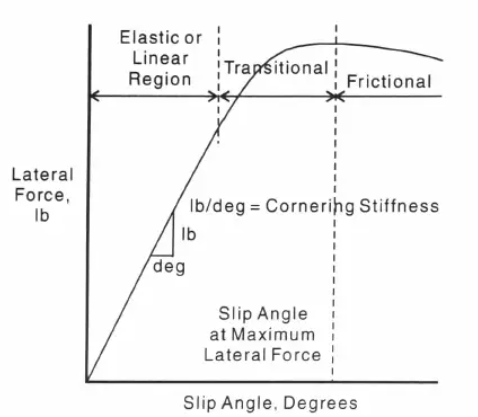
\includegraphics[width=0.6\textwidth]{figures/force-vs-slip_haney2004.png}
    \end{center}
    \caption{Περιοχές προσκόλλησης - ολίσθησης \cite{haney2025racing}}
    \label{fig:load_slip_curve_regions}
\end{figure}

Στην πραγματική λειτουργία, η διαμήκης και η πλευρική ολίσθηση
εμφανίζονται συχνά ταυτόχρονα. Η κατάσταση αυτή ονομάζεται συνδυασμένη
ολίσθηση. Για παράδειγμα, κατά την πέδηση μέσα σε στροφή, μέρος της
διαθέσιμης πρόσφυσης χρησιμοποιείται για την παραγωγή διαμήκους δύναμης
και το υπόλοιπο για την παραγωγή πλευρικής δύναμης. Για τον λόγο αυτό,
η μέγιστη πλευρική ή διαμήκης δύναμη μειώνεται όταν το ελαστικό
λειτουργεί ταυτόχρονα σε πέδηση ή επιτάχυνση και σε πλευρική ολίσθηση
\cite{Pacejka2012,Perantoni2014}. Στο ιδεατό ανάλογο μοντέλο brush, αυτό
θα ήταν άμεσα προφανές αν θεωρήσει κανείς τις ίνες της βούρτσας ως ισοτροπικές.
Σε αυτή την περίπτωση, σε κάθε διεύθυνση καθεμία ίνα έχει την ίδια διαθέσιμη
πρόσφυση, οπότε αγνοώντας τη γεωμετρία του ελαστικού, σε ένα επίπεδο διαμήκους και
πλευρικής δύναμης, η διαθέσιμη πρόσφυση του ελαστικού θα περιγραφόταν με έναν τέλειο κύκλο.
Ένα τέτοιο διάγραμμα ονομάζεται traction envelope. Στην πραγματικότητα 
τα ελαστικά λόγω της κατασκευής τους αλλά και της γεωμετρίας τους,
παρουσιάζουν ανισότροπη συμπεριφορά, και το traction envelope συνήθως
έχει τη μορφή έλλειψης, γι' αυτό και καλείται συχνά traction ellipse. 

\paragraph{Φαινόμενο load sensitivity.}
Ο συντελεστής τριβής $\mu$ δεν είναι σταθερός αλλά μειώνεται ελαφρά καθώς αυξάνεται το
κατακόρυφο φορτίο.

Η φυσική βάση αυτού του φαινομένου έγκειται στη μη-γραμμική ελαστικότητα του ελαστομερούς
υπό πίεση: σε μεγάλα φορτία ο μηχανισμός προσκόλλησης φτάνει σε κορεσμό. Πρακτικά, αυτό σημαίνει
ότι κατά τη μεταφορά φορτίου σε μια στροφή ο επιφορτισμένος τροχός κερδίζει λιγότερη πρόσφυση
από ό,τι χάνει ο αποφορτισμένος. Αυτός ο μηχανισμός είναι και στο μεγαλύτερο βαθμό ο λόγος για τον
οποίο επιθυμείται χαμηλό κέντρο βάρους σε αγωνιστικές εφαρμογές (\cref{eq:longitudinalWeightTransfer,eq:lateralWeightTransfer})
-- ελαχιστοποιώντας το ύψος του κέντρου βάρους ελαχιστοποιούμε και το ποσό πρόσφυσης που "χάνεται".


\paragraph{Μαθηματικά μοντέλα ελαστικών}
Είναι προφανές λοιπόν πως τα ελαστικά αποτελούν ίσως τον σημαντικότερο
παράγοντα στις επιδόσεις ενός οχήματος και η ακριβής μοντελοποίησή τους
χρήζει ιδιαίτερου ενδιαφέροντος. Στην πράξη, λόγω και της έντονης πολυπλοκότητας
στους μηχανισμούς ανάπτυξης φορτίων, χρησιμοποιούνται ημιεμπειρικά παραμετρικά 
μαθηματικά μοντέλα τέτοιας μορφής όπως στις (\cref{eq:longitudinal_tyre_force,eq:lateral_tyre_force}) τα οποία σχεδιάζονται έτσι ώστε να μπορούν να αποτυπώσουν
τη συμπεριφορά των ελαστικών όσο το δυνατό ακριβέστερα προσαρμόζοντάς τα σε 
πειραματικά δεδομένα. Ίσως το πιο διαδεδομένο ημιεμπειρικό μοντέλο πλέον είναι
η Magic Formula του Pacejka \cite{Pacejka2012,Sakhnevych2022}.

\begin{equation}
F_x = F_x\left(F_z,\kappa,\alpha\right),
\label{eq:longitudinal_tyre_force}
\end{equation}

\begin{equation}
F_y = F_y\left(F_z,\kappa,\alpha\right).
\label{eq:lateral_tyre_force}
\end{equation}


\subsubsection{Επίδραση θερμοκρασίας}
\label{subsubsec:temp_effect}
Η πρόσφυση του ελαστικού παρουσιάζει έντονα μη γραμμική εξάρτηση από τη
θερμοκρασία του πέλματος. Σε μια τυπική συμπεριφορά ενός αγωνιστικού ελαστικού
καθώς η θερμοκρασία αυξάνεται, η διαθέσιμη πρόσφυση αρχικά αυξάνεται 
μέχρι ένα βέλτιστο εύρος θερμοκρασίας (παράθυρο λειτουργίας) και στη
συνέχεια ακολουθεί μια πτώση καθώς το ελαστικό εξέρχεται από το παράθυρο λειτουργίας.
Το παράθυρο λειτουργίας δεν είναι μια καθολική ιδιότητα, 
αλλά εξαρτάται έντονα από τη χημική σύνθεση του ελαστικού, το επίπεδο φθοράς κ.ά.
Για παράδειγμα, αναφέρεται στην έρευνα των West, Limebeer \cite{West2022}
πως η βέλτιστη πρόσφυση σε ένα αγωνιστικό ελαστικό εμφανίζεται 
σε θερμοκρασία πέλματος περίπου μεταξύ $90\degC$ και
$105\degC$. Επομένως, σε ένα μοντέλο οχήματος που
δεν περιορίζεται σε ιδανικές, σταθερές συνθήκες ελαστικών, η μοντελοποίηση της επίδρασης της θερμοκρασίας
παίζει πολύ σημαντικό ρόλο στις τελικές επιδόσεις του οχήματος. Άλλωστε, σε
αγωνιστικές εφαρμογές, ειδικότερα στο Παγκόσμιο Πρωτάθλημα Formula 1, όπου
τα ελαστικά είναι ιδιαίτερα ευαίσθητα στη θερμοκρασία, μεγάλο μέρος της
στρατηγικής του αγώνα, του σχεδιασμού (βλ. DAS \cite{WikipediaDualAxisSteering}),
των παραμέτρων ευθυγράμμισης κ.ά. αφορούν τη διαχείριση θερμοκρασίας.

Σε φυσικό επίπεδο, η θερμοκρασία του πέλματος επηρεάζει την πρόσφυση επειδή
μεταβάλλει τις ιξωδοελαστικές ιδιότητες του ελαστομερούς. Η τριβή
ελαστικού και οδοστρώματος σε μοριακό επίπεδο αποδίδεται σε
συνεισφορές που σχετίζονται με τη μοριακή προσκόλληση και με τις απώλειες
παραμόρφωσης του ελαστικού από τις ανωμαλίες του οδοστρώματος (υστέρηση). 
Η μεταβολή της θερμοκρασίας αλλάζει τη δυναμική απόκριση και τους χρόνους 
χαλάρωσης του ελαστομερούς \cite{Grosch1963}. Επιπλέον, η αύξηση της θερμοκρασίας αυξάνει τη
δραστικότητα του πολυμερούς αυξάνοντας τις δυνάμεις προσκόλλησης (chemical adhesion). Η πτώση
της πρόσφυσης με την περαιτέρω αύξηση της θερμοκρασίας αποδίδεται ως επί το πλείστον
στον εκφυλισμό των φυσικών ιδιοτήτων του, ενώ επίσης στο εξωτερικό στρώμα του πέλματος
επιταχύνεται η φθορά και η πρόσφυση περιορίζεται από την 
αντοχή του ίδιου του πέλματος.

\subsection{Μηχανισμοί παραγωγής θερμότητας}
\label{subsec:heat_gen}

Το σύνολο της θερμότητας που παράγεται στον τροχό προέρχεται κυρίως από το ελαστικό
και το σύστημα πέδησης. Ενώ η θερμότητα του συστήματος πέδησης μπορεί να επηρεάσει σημαντικά
τον όγκο ελέγχου του τροχού, στην παρούσα εργασία θα εστιάσουμε στην παραγωγή θερμότητας από
τα ελαστικά θεωρώντας πως δεν υπάρχει συναλλαγή με το σύστημα πέδησης, άλλωστε σε αρκετές
έρευνες έχει χρησιμοποιηθεί αυτή η θεώρηση με αξιοσημείωτη ακρίβεια \cite{West2022, Tremlett2016}.

Η ενέργεια που εισέρχεται στο ελαστικό κατά τη λειτουργία προέρχεται από δύο ξεχωριστές
φυσικές διεργασίες. Η πρώτη και κυρίαρχη σε έντονες μανούβρες είναι η \emph{τριβή
ολίσθησης} (sliding friction) στο πέλμα: όταν υπάρχει σχετική κίνηση μεταξύ
ελαστικού και οδοστρώματος, το μηχανικό έργο της τριβής μετατρέπεται σχεδόν εξ ολοκλήρου σε
θερμότητα. Ο ρυθμός αυτής της παραγωγής εξαρτάται τόσο από την ένταση των δυνάμεων στο
πέλμα (εφαπτομενικές δυνάμεις $F_x$, $F_y$) όσο και από τον βαθμό ολίσθησης, που
χαρακτηρίζεται από τον λόγο ολίσθησης $\kappa$ και τη γωνία ολίσθησης $\alpha$.

Η δεύτερη πηγή είναι η \emph{υστέρηση} (hysteresis) του σκελετού του ελαστικού: το ελαστομερές δεν
συμπεριφέρεται ως ιδανικά ελαστικό υλικό αλλά ως ιξωδοελαστικό -- κατά την κυκλική φόρτισή
του (κάθε στροφή του τροχού) ένα μέρος της παραμορφωτικής ενέργειας δεν αποκαθίσταται αλλά
αποδίδεται ως θερμότητα. Αυτός ο μηχανισμός είναι σημαντικός ακόμα και απουσία ολίσθησης.

Αξίζει να σημειωθεί η συμβολή του κατακόρυφου φορτίου $F_z$: η κάμψη του πλευρικού τοιχώματος
-- εντονότερη υπό μεγαλύτερο φορτίο -- συνεισφέρει σημαντικά στην παραγωγή θερμότητας, 
ακόμη και χωρίς ιδιαίτερα υψηλές πλευρικές και διαμήκεις επιταχύνσεις.
Οι Farroni κ.ά. \cite{Farroni2014TRT} αναλύουν αυτόν
τον μηχανισμό λεπτομερώς στο πλαίσιο ενός τρισδιάστατου θερμικού
μοντέλου πεπερασμένων στοιχείων.

% ------------------------------------------------------------------
\subsection{Μηχανισμοί απαγωγής θερμότητας}
\label{subsec:heat_diss}
% ------------------------------------------------------------------
Η θερμοκρασία μόνιμης κατάστασης του πέλματος καθορίζεται από τη θερμότητα που παράγεται
αλλά και από εκείνη που απάγεται. Δύο κύριοι μηχανισμοί απαγωγής δρουν ταυτόχρονα κατά τη
λειτουργία.

Ο πρώτος είναι η \emph{συναγωγή με τον αέρα} (convective cooling) λόγω της έκθεσης του ελαστικού
σε ροή αέρα εξωτερικά. Η ψύξη αυτή εξαρτάται από τη διαφορά θερμοκρασίας
επιφάνειας–αέρα και από τη σχετική ταχύτητα. Η γενική εξίσωση συναγωγής φαίνεται στην \cref{eq:convection},
ο συντελεστής συναγωγής είναι τυπικά της μορφής $h = \alpha V^n$ επομένως επηρεάζεται κυρίως
από την ταχύτητα του οχήματος και είναι ο βασικότερος μηχανισμός που το ελαστικό απάγει θερμότητα.
Ωστόσο, ειδικά σε αγωνιστικές εφαρμογές, δεν είναι πάντα λύση να εκτεθεί στη ροή του αέρα (ή να προστεθεί
αεραγωγός ψύξης προς το ελαστικό). Τα αγωνιστικά οχήματα είναι πολύ ευαίσθητα στον ομόρρου που δημιουργείται
από τα ελαστικά ο οποίος αυξάνει την αεροδυναμική αντίσταση \cite{tyreWake}, οπότε στην πράξη οι σχεδιαστές προτιμούν
να περιορίσουν την έκθεση του ελαστικού στη ροή, και εφόσον χρειαστεί η θερμοκρασία των ελαστικών ελαττώνεται 
περιορίζοντας την παραγωγή θερμότητας. 


\begin{equation}
    Q_{\text{συναγωγή}} = hA(T_{\text{πέλμα}} - T_{\text{αέρας}})
    \label{eq:convection}
\end{equation}


Ο δεύτερος μηχανισμός είναι η \emph{αγωγιμότητα με το οδόστρωμα} (tyre-road conduction).
Στο πέλμα, όπου το ελαστικό πιέζεται πάνω στην άσφαλτο, υπάρχει άμεση ανταλλαγή
θερμότητας \cref{eq:conduction}.

\begin{equation}
    Q_{αγωγή} = \dfrac{T_{\text{πέλμα}} - T_{\text{οδοστ.}}}{R_{\text{επαφής}}}
    \label{eq:conduction}
\end{equation}

Σημειώνεται εδώ πως η θερμότητα $Q_{\text{αγωγή}}$ μπορεί να είναι αρνητική -- δηλαδή ο
δρόμος να \emph{θερμαίνει} το ελαστικό -- ειδικά κατά τους πρώτους γύρους με κρύα
ελαστικά, εφόσον $T_{\text{οδόστρωμα}} > T_{\text{πέλμα}}$. Αυτό
συμβαίνει ιδιαίτερα λόγω του μηχανισμού αγωγής, διότι συνήθως (και ειδικότερα
το καλοκαίρι ή το μεσημέρι) το οδόστρωμα είναι αρκετούς βαθμούς θερμότερο
από τη θερμοκρασία περιβάλλοντος.

% ============================================================
%  Μηχανισμοί φθοράς αγωνιστικού ελαστικού -- θεωρητικό υπόβαθρο
% ============================================================
\subsection{Μηχανισμοί φθοράς}

Η φθορά ενός ελαστικού είναι το τελικό αποτέλεσμα ενός συνόλου τριβολογικών, θερμικών
και χημικών διεργασιών που εξελίσσονται στη διεπαφή πέλματος-οδοστρώματος. Η φθορά 
των ελαστομερών προκύπτει από τη συνύπαρξη πολλών φαινομένων, η
σχετική βαρύτητα των οποίων εξαρτάται από τη θερμοκρασία, την πίεση επαφής, την ταχύτητα
ολίσθησης και την τραχύτητα του δρόμου. Στα αγωνιστικά ελαστικά, η κατανόηση αυτών των μηχανισμών
είναι σημαντική αφενός για τον σχεδιασμό στρατηγικής αγώνα και αφετέρου για τη σωστή μοντελοποίησή
τους.

Σκοπός του κεφαλαίου είναι η ποιοτική περιγραφή των φυσικών φαινομένων που κυριαρχούν στη
φθορά του πέλματος. Σημειώνεται πως στην παρούσα εργασία η φθορά εκφράζεται κατ' απόλυτο τρόπο, 
ως η ελάττωση της ακτίνας του ελαστικού από κάποιο σημείο αναφοράς και εκφράζεται σε 
$mm$. Συχνά, η έννοια της φθοράς συναντάται ως ένα πιο αφηρημένο μέγεθος και ονομάζεται
ενέργεια ελαστικού (tyre energy), που εκφράζει το ολοκλήρωμα της "ισχύος φθοράς".
Χρησιμοποιείται συχνά για να περιγράψει ποιοτικά την εναπομείνουσα "ζωή" του ελαστικού.
Οι μαθηματικές εκφράσεις των αντίστοιχων μηχανισμών, καθώς και η
ενσωμάτωσή τους στο μοντέλο ελαστικού, παρουσιάζονται στο επόμενο κεφάλαιο.

% ---
\subsubsection{Κατηγοριοποίηση μηχανισμών φθοράς}
\label{subsubsec:wear_classes}
% ---

Στην τριβολογική βιβλιογραφία, η φθορά επιφανειών
που έρχονται σε επαφή διακρίνεται σε τέσσερις κύριες κατηγορίες \cite{WangKTH2017,Grosch1963}.

\paragraph{Προσκολλητική (adhesive) φθορά.}
Οφείλεται στη διάσπαση των μοριακών δεσμών που σχηματίζονται μεταξύ ελαστομερούς και οδοστρώματος στο
πέλμα καθώς οι δύο επιφάνειες αποκτούν σχετική ταχύτητα. Η θραύση των
δεσμών αυτών συνοδεύεται είτε από αποκόλληση υλικού από το ελαστικό είτε από μεταφορά
υλικού στην άσφαλτο. Η ένταση του φαινομένου εξαρτάται από τη χημεία του ελαστομερούς,
την τραχύτητα του οδοστρώματος και τη θερμοκρασία επαφής. Η αύξηση της φθοράς με τη 
θερμοκρασία περιγράφει επίσης την πτώση της μέγιστης πρόσφυσης που περιγράφηκε στο 
\cref{subsubsec:temp_effect}.

\paragraph{Αποξεστική (abrasive) φθορά.}
Εμφανίζεται όταν οι μικροανωμαλίες του σκληρότερου σώματος (των κόκκων του
οδοστρώματος) εισχωρούν στο μαλακότερο υλικό (το ελαστομερές) και αποκόπτουν
μικροσκοπικά τμήματά του. Αποτελεί μηχανισμό καθαρά μηχανικής φθοράς και είναι
ο κυρίαρχος μηχανισμός υπό κανονικές συνθήκες λειτουργίας ενός
ελαστικού.

\paragraph{Φθορά κόπωσης (fatigue wear).}
Προκύπτει από την επαναληπτική φόρτιση της επιφάνειας κατά την κύλιση: κάθε στοιχείο του
πέλματος υπόκειται σε κυκλική διάτμηση και, όταν το πλάτος αυτής
της φόρτισης υπερβεί το όριο κόπωσης του υλικού, εμφανίζονται μικρορωγμές που τελικά
οδηγούν σε αποκόλληση υλικού. Είναι δευτερεύων μηχανισμός στη συνήθη λειτουργία, αλλά
αποκτά σημασία σε μεγάλες διαδρομές και σε συνθήκες υψηλού κατακόρυφου φορτίου.

\paragraph{Χημική και διαβρωτική φθορά.}
Περιλαμβάνει την οξείδωση του ελαστομερούς λόγω θερμοκρασίας και έκθεσης στο περιβάλλον,
καθώς και τη διάβρωση από σωματίδια που παρασύρονται από τη ροή αέρα ή από νερό στην
επιφάνεια του δρόμου. Στην αγωνιστική οδήγηση, με τα σχετικά μικρά μήκη αγώνα και τις
ελεγχόμενες συνθήκες, τα φαινόμενα αυτά είναι πρακτικά αμελητέα.

Στο πλαίσιο της παρούσας εργασίας το ενδιαφέρον εστιάζεται στην αποξεστική και στην
προσκολλητική φθορά. Η φθορά κόπωσης και η χημική φθορά αναπτύσσονται σε πολύ μεγαλύτερες
αποστάσεις από τη διάρκεια ζωής ενός αγωνιστικού ελαστικού, επομένως δεν συνεισφέρουν ουσιαστικά
και αναφέρονται συνοπτικά για πληρότητα.

% ---
\subsubsection{Η θεωρία των δύο μηχανισμών τριβής ελαστομερούς}
\label{subsubsec:two_mechanism}
% ---

Ένα από τα πλέον διαδεδομένα ερμηνευτικά σχήματα για τη φθορά ελαστομερών είναι η λεγόμενη
\emph{θεωρία των δύο μηχανισμών} (two-mechanism theory), η οποία διατυπώθηκε αρχικά από
τους Grosch και Schallamach \cite{Grosch1963} και έχει επαληθευτεί πειραματικά στη σύγχρονη
βιβλιογραφία \cite{Veirh1992,West2022}. Σύμφωνα με αυτή, ο ρυθμός φθοράς κυριαρχείται από
δύο μηχανισμούς και παρουσιάζει χαρακτηριστική $U$-μορφή ως προς τη θερμοκρασία, με ελάχιστο
κοντά στο παράθυρο πρόσφυσης και έντονη αύξηση εκατέρωθεν (\cref{fig:twoMechanismTheory}).

Ο πρώτος μηχανισμός κυριαρχεί σε χαμηλές θερμοκρασίες, όπου το ελαστομερές συμπεριφέρεται
περισσότερο σαν υαλώδες υλικό. Οι μικροανωμαλίες του οδοστρώματος ασκούν εντοπισμένες τάσεις
στην επιφάνεια του πέλματος και, λόγω της αυξημένης δυσκαμψίας του υλικού, αυτές οδηγούν
σε ψαθυρή θραύση αντί για ελαστική παραμόρφωση. Το αποτέλεσμα είναι η αποκόλληση
σωματιδίων ελαστομερούς με μηχανισμό διάδωσης ρωγμών
\cite{West2022}. Ο μηχανισμός αυτός ευνοείται σε οδοστρώματα με υψηλή μικροϋφή και σε
σκληρότερες συνθέσεις ελαστικών.

Ο δεύτερος μηχανισμός γίνεται κυρίαρχος σε υψηλές θερμοκρασίες, όπου η θερμική ενέργεια
είναι επαρκής ώστε οι διακυμαινόμενες διατμητικές τάσεις που ασκούνται από τις
μικροανωμαλίες του δρόμου να σπάνε μοριακούς δεσμούς εντός του υλικού
\cite{West2022,Grosch1963}. Πρόκειται δηλαδή για μια θερμικά ενεργοποιημένη διεργασία
θραύσης δεσμών, η οποία εξηγεί την απότομη αύξηση του ρυθμού φθοράς όταν η θερμοκρασία
πέλματος ξεπεράσει το ανώτερο όριο του θερμικού παραθύρου. Ο μηχανισμός αυτός ευνοείται
από χαμηλή μικροϋφή (λείο οδόστρωμα), μαλακότερα ελαστομερή και υψηλές ταχύτητες ολίσθησης.

\begin{figure}[ht!]
    \begin{center}
        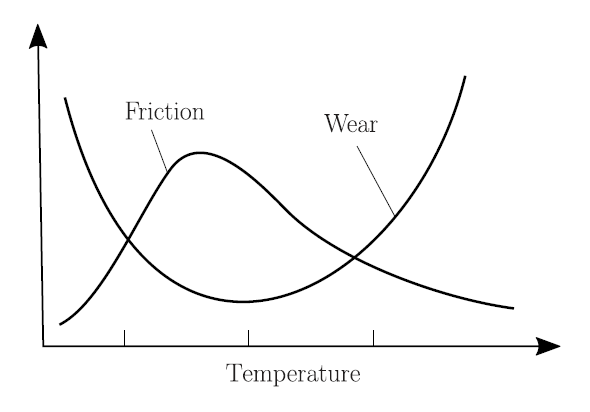
\includegraphics[width=0.6\textwidth]{figures/wear-vs-temperature.png}
    \end{center}
    \caption{Συσχέτιση ρυθμού φθοράς με θερμοκρασία \cite{persson2001}}
    \label{fig:twoMechanismTheory}
\end{figure}

Το κρίσιμο συμπέρασμα της θεωρίας των δύο μηχανισμών είναι πως η ελαχιστοποίηση της
φθοράς και η μεγιστοποίηση της πρόσφυσης δεν είναι ανταγωνιστικές απαιτήσεις ως προς τη θερμοκρασία: και οι δύο
επιτυγχάνονται όταν το ελαστικό λειτουργεί εντός του σχετικά στενού θερμικού παραθύρου.
Αυτή η παρατήρηση τεκμηριώνει τη σκοπιμότητα να αντιμετωπιστεί η θερμική διαχείριση των
ελαστικών ως το κύριο πρόβλημα στρατηγικής αγώνα \cite{West2022,Tremlett2016}.

% ---
\subsubsection{Μακροσκοπικά φαινόμενα: σχηματισμός κόκκων (graining) και φυσαλίδων (blistering)}
\label{subsubsec:graining_blistering}
% ---

Οι δύο μηχανισμοί της προηγούμενης παραγράφου εκδηλώνονται μακροσκοπικά με δύο ξεχωριστά
και άμεσα αναγνωρίσιμα φαινόμενα: το \emph{graining} και το
\emph{blistering}. Το πρώτο αντιστοιχεί στον μηχανισμό χαμηλών θερμοκρασιών, ενώ το
δεύτερο σε αυτόν των υψηλών.

\paragraph{Σχηματισμός κόκκων -- \textit{Graining}.}
Το graining εμφανίζεται όταν το ελαστικό λειτουργεί σε θερμοκρασία \emph{κάτω} από το
κατώτατο όριο του θερμικού παραθύρου του. Σε αυτή τη ζώνη, η δυσκαμψία του ελαστομερούς
είναι υψηλή και η προσκόλληση με το οδόστρωμα σχετικά χαμηλή. Αντί δηλαδή η επιφάνεια να
τρίβεται με ομαλό τρόπο, τείνει να αποκολλά μικρά τεμάχια τα οποία στη συνέχεια
επικολλώνται εκ νέου στο πέλμα, δημιουργώντας μια χαρακτηριστική κοκκώδη υφή. Η υφή αυτή
μειώνει την ενεργή επιφάνεια επαφής και αυξάνει την τραχύτητα του πέλματος, με αποτέλεσμα
την περαιτέρω μείωση της πρόσφυσης και την επιτάχυνση του ίδιου του φαινομένου (\cref{fig:graining}).

Ένα χαρακτηριστικό γνώρισμα του \textit{graining} είναι η \emph{εν μέρει αναστρέψιμη} φύση του: αν
το ελαστικό καταφέρει να ανεβάσει θερμοκρασία και να μπει εντός του θερμικού παραθύρου, η
θερμική ενέργεια μπορεί να εξομαλύνει τμήμα της κοκκώδους υφής, αποκαθιστώντας
μέρος της αρχικής πρόσφυσης. 

\paragraph{Σχηματισμός φυσαλίδων -- \textit{Blistering}.}
Το \textit{blistering} συναντάται στην άλλη πλευρά του παραθύρου λειτουργίας και εμφανίζεται
όταν το ελαστικό λειτουργεί \emph{πάνω} από το ανώτατο όριο του θερμικού παραθύρου, δηλαδή σε κατάσταση υπερθέρμανσης.
Οι υψηλές θερμοκρασίες οδηγούν σε τοπικό "μαλάκωμα" των στρωμάτων του ελαστομερούς κάτω από την επιφάνεια
και ως αποτέλεσμα εξατμίζονται πρόσθετα του ελαστομερούς (\textit{outgassing}) και παγιδεύονται εντός του υλικού.
Τα αέρια αυτά σχηματίζουν φυσαλίδες (blisters) κάτω από την επιφάνεια οι οποίες, όταν
τελικά σκάσουν, εκτινάσσουν κομμάτια πέλματος αφήνοντας ακανόνιστους "κρατήρες" (\cref{fig:blistering}).

Σε αντίθεση με το \textit{graining}, το \textit{blistering} είναι \emph{μη αναστρέψιμο}: μόλις σχηματιστούν
φυσαλίδες, η δομική βλάβη έχει ήδη συμβεί και δεν αναιρείται με μεταγενέστερη ψύξη του
ελαστικού. 

\begin{figure}[htbp]
    \centering
    \begin{subfigure}[t]{0.48\textwidth}
        \centering
        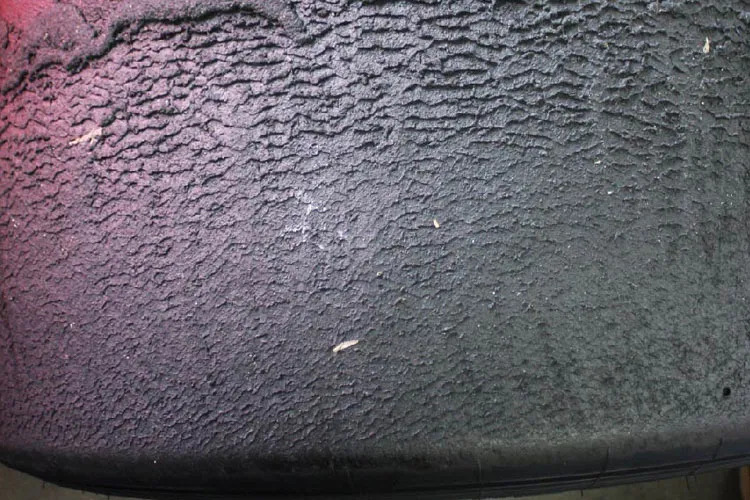
\includegraphics[height=5cm]{figures/Tyre-graining.jpg}
        \caption{\textit{Graining} -- κόκκοι στην επιφάνεια του πέλματος.}
        \label{fig:graining}
    \end{subfigure}
    \hfill
    \begin{subfigure}[t]{0.48\textwidth}
        \centering
        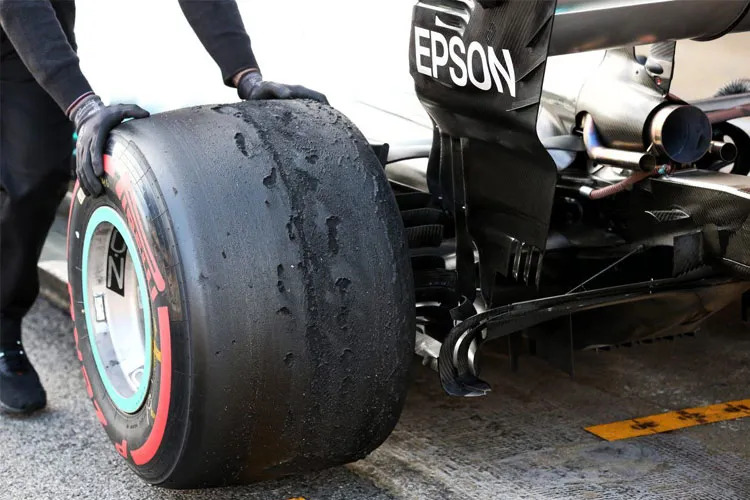
\includegraphics[height=5cm]{figures/Tyre-blistering.jpg}
        \caption{\textit{Blistering} -- σχηματισμός φυσαλίδων και αποκόλληση υλικού.}
        \label{fig:blistering}
    \end{subfigure}
    \caption{Τα δύο μακροσκοπικά φαινόμενα φθοράς ελαστικού \cite{suspensionsecrets2020tyre}.}
    \label{fig:graining_vs_blistering}
\end{figure}

% ---
\subsubsection{Επίδραση κατακόρυφου φορτίου, πίεσης και γεωμετρίας ανάρτησης}
\label{subsubsec:wear_secondary}
% ---

Πέρα από τη θερμοκρασία, ο ρυθμός φθοράς επηρεάζεται από παράγοντες που σχετίζονται με τη
γεωμετρία και τη δυναμική του οχήματος. Το κατακόρυφο φορτίο $F_z$ καθορίζει άμεσα τόσο
την κατανομή της πίεσης όσο και το μέγεθος της επιφάνειας του πέλματος -- και οι δύο ποσότητες υπεισέρχονται
στους υπολογισμούς του έργου τριβής και συνεπώς της συσσωρευμένης θερμότητας. Σύμφωνα με
πειραματικές μετρήσεις σε ελαστικά επιβατικού οχήματος, η φθορά αυξάνεται περίπου γραμμικά
με το κατακόρυφο φορτίο εντός του κανονικού εύρους λειτουργίας \cite{WangKTH2017}.

Η πίεση αέρα του ελαστικού επιδρά έμμεσα: υψηλότερη πίεση αέρα μειώνει την επιφάνεια του πέλματος,
και συνεπώς αυξάνει τη μέγιστη πίεση στο κέντρο του πέλματος. Αυτό αφενός αυξάνει την ένταση της
φθοράς και αφετέρου προκαλεί ανομοιόμορφη φθορά συγκεντρώνοντάς την στο κέντρο του ελαστικού.
Αντιστρόφως, με αντίστοιχο μηχανισμό, χαμηλότερη πίεση μετακινεί τη μέγιστη πίεση επαφής
στις άκρες του πέλματος -- κοντά στα πλαϊνά τοιχώματα, όπου συγκεντρώνεται η φθορά. Το ίδιο ισχύει
και για μη μηδενική γωνία camber ή toe, που μπορούν να προκαλέσουν έντονη
ασύμμετρη φθορά στη μία πλευρά του πέλματος -- φαινόμενα γνωστά στη βιβλιογραφία ως
\emph{camber wear} και \emph{feathered wear} αντίστοιχα \cite{WangKTH2017}.

Στο πλαίσιο του μοντέλου που αναπτύσσεται στην παρούσα εργασία, η γεωμετρία της ανάρτησης
θεωρείται σταθερή (με μηδενικές γωνίες) και οι μεταβολές πίεσης δεν λαμβάνονται υπόψη.
Μελετάται δηλαδή η συνολική φθορά του ελαστικού και όχι η κατανομή και η μορφή της στο ελαστικό.
Οι παραπάνω επιδράσεις αναφέρονται εδώ για πληρότητα και αποτελούν φυσικά επόμενα βήματα επέκτασης του
μοντέλου.

% ---
\subsubsection{Σχέση φθοράς και πρόσφυσης}
\label{subsubsec:wear_grip_coupling}
% ---

Ένα εξίσου σημαντικό στοιχείο για την αγωνιστική οδήγηση είναι η σύζευξη της φθοράς με
την πρόσφυση. Καθώς το πέλμα φθείρεται, ο συντελεστής τριβής μειώνεται προοδευτικά,
τόσο λόγω της μεταβολής της τοπικής σύνθεσης της επιφάνειας όσο και λόγω των γεωμετρικών
αλλαγών του πέλματος \cite{West2022,Tremlett2016}. Για αγωνιστικά ελαστικά, στα οποία η
αρχική χημική σύνθεση σχεδιάζεται για μέγιστη πρόσφυση, η επίδραση αυτή είναι εντονότερη σε
σχέση με ελαστικά καθημερινής χρήσης, που σχεδιάζονται για μεγαλύτερη διάρκεια ζωής.
Εξαίρεση αποτελεί η αρχική φάση φθοράς, η οποία παρουσιάζει συχνά ελαφριά αύξηση
πρόσφυσης: τα αγωνιστικά ελαστικά δεν παρέχονται πάντα πλήρως βουλκανοποιημένα, και με τους
πρώτους κύκλους θερμικής φόρτισης και την απομάκρυνση του εξωτερικού στρώματος του πέλματος
οι ιδιότητές τους σταθεροποιούνται \cite{West2022}. Το φαινόμενο αυτό είναι γνωστό ως \emph{scrubbing-in}.

Στο \cref{fig:tractionVsWear} φαίνεται η τυπική μορφή της καμπύλης πρόσφυσης συναρτήσει
της φθοράς.

Η σύζευξη αυτή σημαίνει ότι η μοντελοποίηση της φθοράς δεν αποτελεί απλώς ένα
αριθμητικό αποτέλεσμα αλλά ανατροφοδοτείται άμεσα και για τον χαρακτηρισμό της 
δυναμικής συμπεριφοράς του οχήματος. Καθώς μειώνεται η πρόσφυση, αυξάνεται η 
απαιτούμενη ολίσθηση για την επίτευξη της ίδιας δύναμης,
που με τη σειρά της αυξάνει την παραγόμενη θερμότητα και τον ρυθμό φθοράς. Αυτό το φαινόμενο
αλληλοενίσχυσης των μηχανισμών είναι ένας από τους λόγους για τους οποίους η ταυτόχρονη
μοντελοποίηση θερμοκρασίας και φθοράς στο πλαίσιο ενός προσομοιωτή γύρου έχει πρακτική
αξία, ακόμη και με τις απλοποιήσεις που υιοθετούνται στην παρούσα εργασία.


\begin{figure}[ht!]
    \begin{center}
        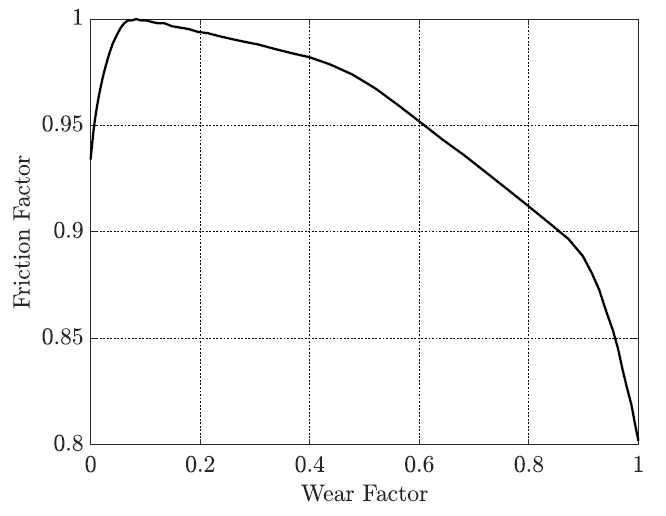
\includegraphics[width=0.6\textwidth]{figures/traction-vs-wear.png}
    \end{center}
    \caption{Συσχέτιση πρόσφυσης με συνολική φθορά \cite{Farroni2019}}
    \label{fig:tractionVsWear}
\end{figure}



\clearoddpage
\section{Μαθηματική \& θερμοδυναμική μοντέλοποίηση ελαστικών}
\label{sec:tyre_model}
\subsection{Συνδυαστικό μοντέλο πρόσφυσης}
% ============================================================
%  §3.1 Συνδυαστικό μοντέλο πρόσφυσης
% ============================================================

\label{subsec:combined_slip}

\subsubsection{Μεγέθη ολίσθησης}

Πριν από την παρουσίαση του μοντέλου, απαιτείται ο αυστηρός ορισμός των βασικών μεγεθών
ολίσθησης. Η έννοια της «ολίσθησης» εκφράζει την απόκλιση μεταξύ της πραγματικής κίνησης
του ελαστικού και της «ιδανικής» κίνησης χωρίς ολίσθηση. Στην πράξη η παραγωγή δυνάμεων
ξεκινά από κινηματική είσοδο -- π.χ. ο οδηγός στρίβει το τιμόνι δημιουργώντας απόκλιση
μεταξύ της στιγμιαίας ταχύτητας των τροχών και της κατεύθυνσής του, ή πιέζει το φρένο
που μειώνει τη γωνιακή ταχύτητα των τροχών. Και στις δυο περιπτώσεις δημιουργείται ολίσθηση
και παράγεται δύναμη στο πέλμα.

\paragraph{Γωνία ολίσθησης $\alpha$ (Slip Angle).}
Ορίζεται ως η γωνία μεταξύ του επιπέδου του τροχού (κατεύθυνση κύλισης) και του
πραγματικού διανύσματος ταχύτητας του κέντρου τροχού:

\begin{equation}
    \alpha = \arctan\!\left(\frac{v_{y}^{\text{ελαστικού}}}{v_{x}^{\text{ελαστικού}}}\right)
    \label{eq:slip_angle}
\end{equation}

όπου $v_{x}^{\text{ελαστικού}}$, $v_{y}^{\text{ελαστικού}}$ οι συνιστώσες ταχύτητας στο επίπεδο
του πέλματος, με διεύθυνση $x$ τη διεύθυνση κύλισης και $y$ κάθετη σε αυτή. Σε καθαρή κύλιση 
$\alpha = 0$. Μη μηδενική $\alpha$ σημαίνει ότι ο τροχός
«γλιστράει» πλευρικά -- έχει εγκάρσια σχετική ταχύτητα με το οδόστρωμα -- 
και αναπτύσσει πλευρική δύναμη $F_y$ (\textit{cornering force}).

% ----- TikZ: slip angle -----
\begin{figure}[htbp]
\centering
\begin{tikzpicture}[scale=1.25,
    wheel/.style={rectangle,draw=black,fill=gray!30,
                  minimum width=0.32cm,minimum height=1.1cm,rounded corners=2pt},
    vec/.style={->,thick}
]
  % wheel
  \node[wheel] (W) at (0,0) {};
  % heading (rolling direction)
  \draw[vec,black!60] (0,-0.9)--(0,1.3)
    node[above,font=\small]{κατεύθυνση τροχού};
  % actual velocity
  \draw[vec,blue!80!black,very thick] (0,0)--(0.65,1.05)
    node[right,font=\small,blue!80!black]{$\mathbf{v}_{\rm wheel}$};
  % alpha arc
  \draw[->,thin,red] (0,0.52) arc[start angle=90,end angle=58,radius=0.52];
  \node[red,font=\small] at (0.3,0.72) {$\alpha$};
  % components
  \draw[dashed,gray!70] (0,1.05)--(0.65,1.05);
  \draw[vec,gray!60] (0,0)--(0.65,0) node[below,font=\scriptsize,gray!60]{$v_y$};
  \draw[vec,gray!60] (0.65,0)--(0.65,1.05) node[right,font=\scriptsize,gray!60]{$v_x$};
\end{tikzpicture}
\caption{Ορισμός γωνίας ολίσθησης $\alpha$. Η διαφορά μεταξύ της πραγματικής ταχύτητας $\mathbf{v}$ και της κατεύθυνσης κύλισης δίνει την $\alpha$, η οποία αντιστοιχεί σε πλευρική δύναμη $F_y$.}
\label{fig:slip_angle}
\end{figure}
% ----- τέλος TikZ -----


\paragraph{Λόγος ολίσθησης $\kappa$ (Slip Ratio).}
Εκφράζει τη σχετική διαφορά μεταξύ της περιφερειακής ταχύτητας τροχού και της ταχύτητας
οχήματος:
\begin{equation}
    \kappa = \frac{\omega \cdot r_{\mathrm{eff}} - v_x}{v_x}
    \label{eq:slip_ratio}
\end{equation}

Για $\kappa = 0$ υπάρχει ιδανική κύλιση (χωρίς ολίσθηση). Θετικές τιμές ($\kappa > 0$) αντιστοιχούν σε
κινητήρια ροπή ενώ αρνητικές ($\kappa < 0$) σε φρενάρισμα. Για $\kappa = -1 (-100\%)$ ο τροχός "μπλοκάρει".

\subsubsection{Μοντέλο συνδυασμένης ολίσθησης}

Όπως αναφέρθηκε και στη θεωρία, τα περισσότερα μαθηματικά μοντέλα ελαστικών 
παίρνουν τη μορφή των εξισώσεων (\ref{eq:longitudinal_tyre_force}) και (\ref{eq:lateral_tyre_force}). 
Η επιλογή του κατάλληλου μοντέλου εξαρτάται από πολλούς παράγοντες, π.χ. αν η συμπεριφορά του ελαστικού
εμφανίζει έντονες μη-γραμμικότητες ή από τα φαινόμενα που θέλουμε να αντικατοπτρίσουμε στο μοντέλο.

Στην παρούσα διπλωματική εργασία επιλέχθηκε ένα σχετικά απλό μοντέλο combined slip 
των \textit{Tremlett \& Limebeer} \cite{Tremlett2016} αφενός διότι περιγράφει με ικανοποιητική
μορφή τα φαινόμενα που θα εξεταστούν, και αφετέρου, διότι επιτρέπει την άμεση σύγκριση των αποτελεσμάτων.

Ωστόσο, το συνολικό μοντέλο είναι δομημένο έτσι ώστε κάθε συνιστώσα του, όπως και το μοντέλο ελαστικών, να είναι ένα τμήμα αποσπασμένο
(modular) έτσι ώστε σε διαφορετική εφαρμογή, όχημα ή ελαστικό
να μπορεί να αντικατασταθεί από μοντέλο που ταιριάζει καλύτερα στις ανάγκες του ή στα 
πειραματικά δεδομένα. \\[0.5cm]

Στον πυρήνα του, το μοντέλο \textit{combined slip} θεωρεί πως η διαθέσιμη πρόσφυση του
ελαστικού σχηματίζει έλλειψη σε ένα επίπεδο πλευρικής-διαμήκους δύναμης.
Το σχήμα της έλλειψης ελέγχεται με τις παραμέτρους $Q_x, Q_y$.

Με τις υπόλοιπες παραμέτρους "κλειδωμένες", η καμπύλη φορτίου--ολίσθησης
(πανομοιότυπη για τη διαμήκη και την πλευρική διεύθυνση) έχει τη μορφή του σχήματος
\ref{fig:force-vs-slip-angle}.

\begin{figure}[ht!]
    \begin{center}
        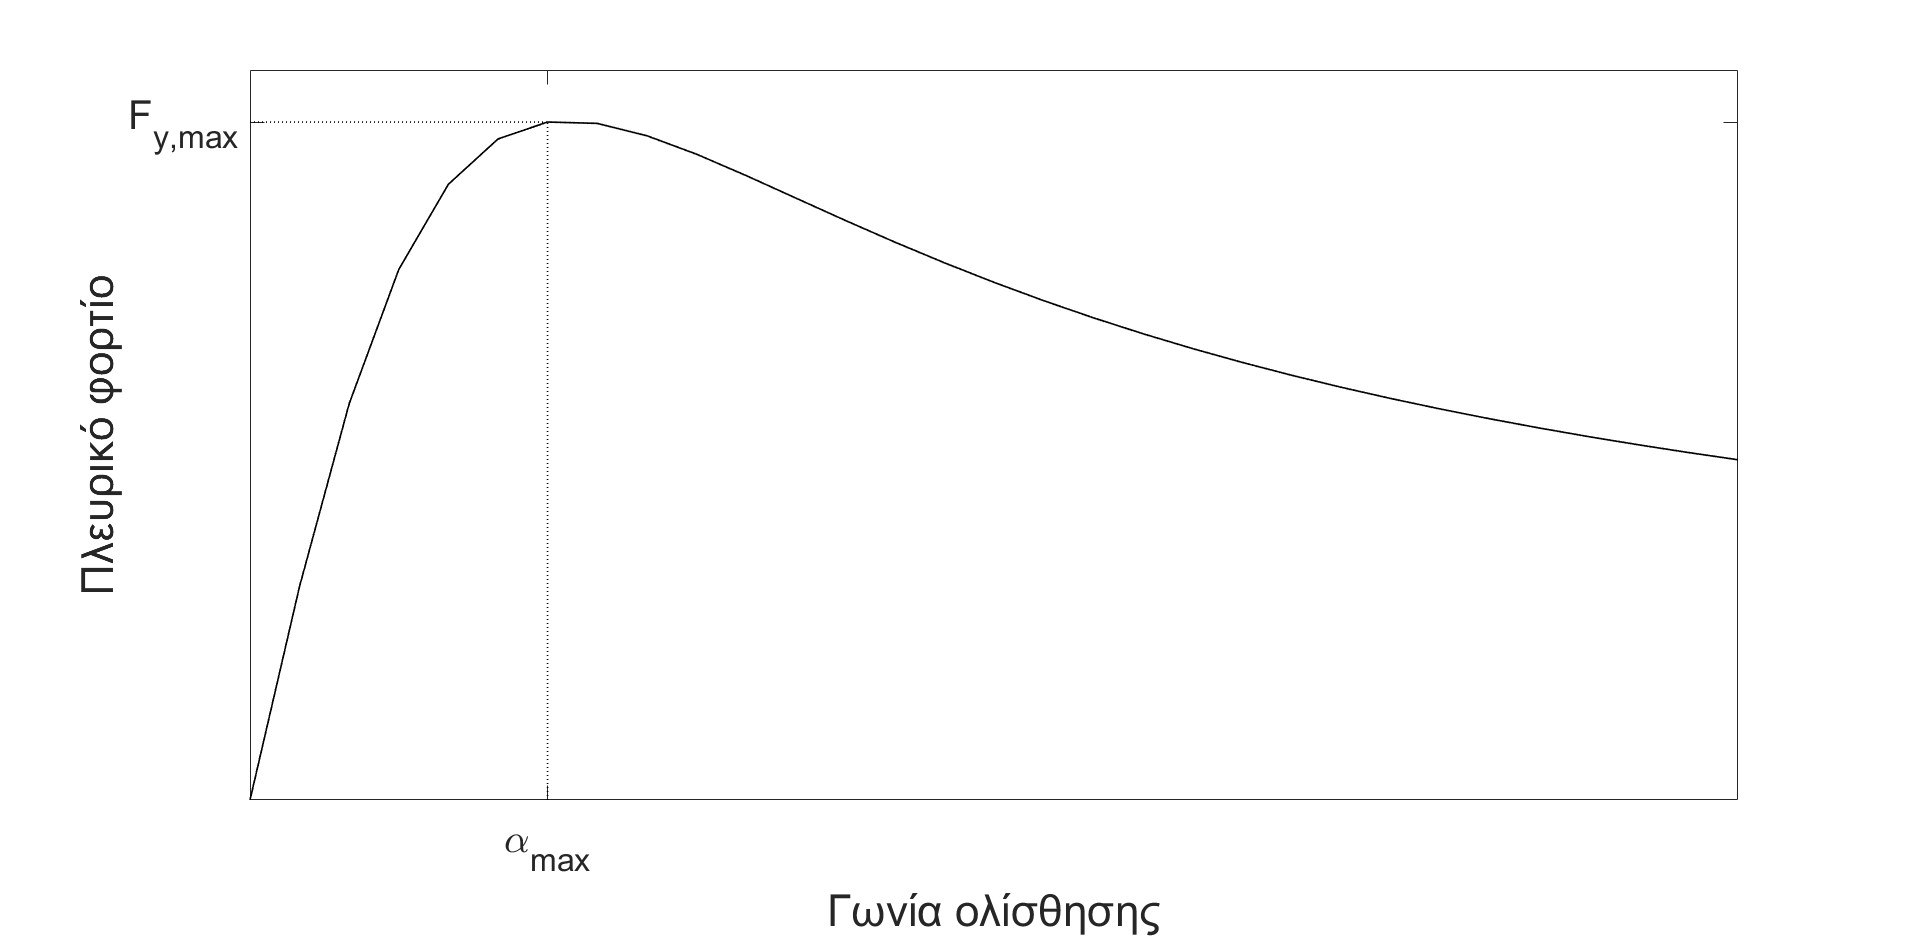
\includegraphics[width=0.8\textwidth]{figures/lateral-tyre.jpg}
    \end{center}
    \caption{Μορφή καμπύλης φορτίου-ολίσθησης}
\label{fig:force-vs-slip-angle}
\end{figure}

Οι τιμές με δείκτη $max$ αναφέρονται στα αντίστοιχα μεγέθη του σημείου μέγιστης δύναμης.

Με βάση τον λόγο και τη γωνία ολίσθησης στην κορυφή, ορίζονται οι αδιάστατοι λόγοι ολίσθησης $\kappa_n, \alpha_n \in [-1,1]$ ως

\begin{align}
    \kappa_n &= \dfrac{\kappa}{\kappa_{max}}\\[10pt]
    \alpha_n &= \dfrac{\alpha}{\alpha_{max}}
\end{align}

Και στη συνέχεια ορίζεται ο αδιάστατος συντελεστής συνδυασμένης ολίσθησης $\rho$ ως:

\begin{equation}
    \rho = \sqrt{\alpha_n^2 + \kappa_n^2}
\end{equation}

Με βάση λοιπόν τα παραπάνω μεγέθη, οι συντελεστές τριβής για τις δύο διευθύνσεις υπολογίζονται ως:

\begin{align}
    \mu_x &= \mu_{x,max}\sin\bigl(Q_xtan^{-1}(
         S_x\rho )\bigr)\\[10pt]
    \mu_y &= \mu_{y,max}\sin\bigl(Q_ytan^{-1}(
         S_y\rho )\bigr)
\end{align}

Με,

\begin{align}
    S_x &= \dfrac{\pi}{2tan^{-1}\bigl(Q_x\bigr)}\\[10pt]
    S_y &= \dfrac{\pi}{2tan^{-1}\bigl(Q_y\bigr)}
\end{align}

Και τέλος, τα διαμήκη και εγκάρσια φορτία ($F_x, F_y$) υπολογίζονται ως

\begin{align}
    F_x &= \mu_xF_z\dfrac{\kappa_n}{\rho}\\[10pt]
    F_y &= \mu_yF_z\dfrac{\alpha_n}{\rho}
\end{align}


\paragraph{Ευαισθησία σε κατακόρυφο φορτίο.}
Ο συντελεστής τριβής $\mu$ δεν είναι σταθερός αλλά μειώνεται ελαφρά καθώς αυξάνεται το
κατακόρυφο φορτίο. Το φαινόμενο αυτό -- όπως περιγράφηκε στο \cref{sec:tyre_theory} -- μοντελοποιείται
με γραμμική παρεμβολή ανάμεσα σε δύο γνωστά σημεία (με δείκτες 1 \& 2).
Καθώς εκτός από το μέγιστο συντελεστή τριβής μεταβάλλεται και το σημείο όπου εμφανίζεται,
παρεμβάλλουμε και τους μέγιστους συντελεστές τριβής ($\mu_{max}$) αλλά και τα αντίστοιχα μεγέθη ολίσθησης στα οποία εμφανίζονται ($\{\alpha, \kappa\}_{max}$).

\begin{align}
    \mu_{x,max}(F_z) &= (F_z - F_{z1})
    \dfrac{\mu_{x,max2} - \mu_{x,max1}}{F_{z2}-F_{z1}} + \mu_{x,max1}
    \label{eq:mu_load1}\\[10pt]
    \mu_{y,max}(F_z) &= (F_z - F_{z1})
    \dfrac{\mu_{y,max2} - \mu_{y,max1}}{F_{z2}-F_{z1}} + \mu_{y,max1}
    \label{eq:mu_load2}\\[10pt]
    \kappa_{max}(F_z) &= (F_z - F_{z1})
    \dfrac{\kappa_{max2} - \kappa_{max1}}{F_{z2}-F_{z1}} + \kappa_{max1}
    \label{eq:mu_load3}\\[10pt]
    \alpha_{max}(F_z) &= (F_z - F_{z1})
    \dfrac{\alpha_{max2} - \alpha_{max1}}{F_{z2}-F_{z1}} + \alpha_{max1}
    \label{eq:mu_load}
\end{align}

\paragraph{Αντιστροφή συνάρτησης}
Όπως αναλύεται στο \cref{sec:inverseModel}, στο μοντέλο της παρούσας εργασίας, οι μεταβλητές εισόδου στο μοντέλο του ελαστικού είναι η γωνία ολίσθησης $\alpha$, το κατακόρυφο φορτίο $F_z$ και το απαιτούμενο διαμήκες φορτίο $F_x$. Επομένως, η επίλυση εμπίπτει στον προσδιορισμό του απαιτούμενου λόγου ολίσθησης $\kappa$ για την επίτευξη του ζητούμενου φορτίου.\\[5pt]
\noindent
Με καθορισμένο κατακόρυφο φορτίο και γωνία ολίσθησης, προκύπτει μονοσήμαντα μία μοναδική καμπύλη $F_x - \kappa$ που έχει τη μορφή του σχήματος (\ref{fig:force-vs-slip-angle}). Η αντιστροφή της συνάρτησης απαιτεί αυστηρό περιορισμό, καθώς δεν είναι 1--1 (\textit{injective}) σε ολόκληρο το πεδίο λόγων ολίσθησης, συγκεκριμένα, η συνθήκη ισχύει μόνο μεταξύ $[-\kappa_{max}, \kappa_{max}]$. Λόγω της φύσης των εξισώσεων, επιλέγεται η αντίστροφη αντιστοίχηση να πραγματοποιηθεί αριθμητικά. Θυσιάζοντας λίγο υπολογιστικό κόστος για ευστάθεια, υπολογίζεται το διαμήκες φορτίο για λόγους ολίσθησης $\kappa \in [-\kappa_{max}, \kappa_{max}]$ και επιλέγεται η τιμή του $\kappa$ που προκαλεί το απαιτούμενο φορτίο $F_x$. Επομένως, σημασιολογικά, η αντίστροφη συνάρτηση του διαμήκους φορτίου έχει τη μορφή της εξίσωσης (\ref{eq:slipRatioInversion}), ενώ επίσης για σκοπούς που αναλύονται σε επόμενα κεφάλαια, υπολογίζεται και το μέγιστο διαμήκες φορτίο που μπορεί να αναπτυχθεί με τις δεδομένες συνθήκες (\cref{eq:maxLongitudinalForce}).

\begin{equation}
    \kappa = f(\alpha, F_z, F_x)
    \label{eq:slipRatioInversion}
\end{equation}


\begin{equation}
    F_{x,max} = f(\alpha, F_z)
    \label{eq:maxLongitudinalForce}
\end{equation}

\noindent
Επομένως, η τελική μορφή του μοντέλου ελαστικών είναι:

\begin{equation}
    (F_y,\kappa)= f(\alpha,F_x, F_z)
    \label{eq:tyreModelFinal}
\end{equation}

% ------------------------------------------------------------
%  1) Συνδυαστικό μοντέλο πρόσφυσης
% ------------------------------------------------------------
\begin{table}[htbp]
    \centering
    \small
    \renewcommand{\arraystretch}{1.2}
    \begin{tabular}{@{}l l l@{}}
        \toprule
        \textbf{Παράμετρος} & \textbf{Τιμή (Μονάδα)} & \textbf{Περιγραφή} \\
        \midrule
        $F_{z1}$     & $2000$ N   & Χαμηλό επίπεδο κατακόρυφου φορτίου αναφοράς \\
        $F_{z2}$     & $6000$ N   & Υψηλό επίπεδο κατακόρυφου φορτίου αναφοράς \\
        $\mu_{x,max1}$ & $1.75$     & Διαμήκης συντ. τριβής στο $F_{z1}$ \\
        $\mu_{x,max2}$ & $1.40$     & Διαμήκης συντ. τριβής στο $F_{z2}$ \\
        $\mu_{y,max1}$ & $1.80$     & Πλευρικός συντ. τριβής στο $F_{z1}$ \\
        $\mu_{y,max2}$ & $1.45$     & Πλευρικός συντ. τριβής στο $F_{z2}$ \\
        $\kappa_{max1}$ & $0.11$     & Μέγιστο slip ratio στο $F_{z1}$ \\
        $\kappa_{max2}$ & $0.10$     & Μέγιστο slip ratio στο $F_{z2}$ \\
        $\alpha_{max1}$ & $9^\circ$  & Μέγιστη γωνία slip στο $F_{z1}$ \\
        $\alpha_{max2}$ & $8^\circ$  & Μέγιστη γωνία slip στο $F_{z2}$ \\
        $Q_x$        & $1.9$      & Παράμετρος καμπυλότητας διαμήκους καμπύλης \\
        $Q_y$        & $1.9$      & Παράμετρος καμπυλότητας πλευρικής καμπύλης \\
        $\mu_{\min}$ & $0.20$     & Κάτω κατώφλι συντ. τριβής (friction clamp) \\
        \bottomrule
    \end{tabular}
    \caption{Παράμετροι συνδυαστικού μοντέλου πρόσφυσης (combined slip).}
    \label{tab:params_combined}
\end{table}

\paragraph{Εξάρτηση με θερμοκρασία και φθορά.}

Τελικά, οι υπολογισμένοι συντελεστές τριβής πολλαπλασιάζονται με συντελεστές μείωσης,
έναν για τη διόρθωση λόγω θερμοκρασίας και έναν για τη διόρθωση λόγω φθοράς.

\begin{equation}
    \mu_{\rm eff}(F_z, T, w) = \mu(F_z) \cdot \lambda(T)\cdot\gamma(w)
    \label{eq:mu_temp_wear}
\end{equation}

όπου $\lambda(T)$ ο συντελεστής μείωσης λόγω θερμοκρασίας και $\gamma(w)$ ο συντελεστής μείωσης λόγω φθοράς. 


\subsection{Εξάρτηση πρόσφυσης από θερμοκρασία}

Ο λόγος μείωσης της πρόσφυσης μοντελοποιείται εμπειρικά ακολουθώντας ποιοτικά τη μορφή του σχήματος \ref{fig:twoMechanismTheory}, χρησιμοποιώντας τρεις γραμμικές περιοχές με ομαλή μετάβαση για αριθμητική ευστάθεια.


\begin{equation}
\begin{aligned}
   \lambda(T_s) = \bigl(g_1T_s +g_2\bigr) + &\Bigl(0.5
   +0.5sin\Bigl(tan^{-1}\bigl(g_s(T_s-T_{p1})\bigr)\Bigr)\Bigr)\cdot\Bigl(1-(g_1T_s+g_2)\Bigr)\\[6pt]
   + &\Bigl(0.5 + 0.5sin\Bigl(tan^{-1}\bigl(g_s(T_s-T_{p2})\bigr)\Bigr)\Bigr)\cdot
   \Bigl(\bigl(g_3T_s+g_4\bigr)-1\Bigr)
\end{aligned}
\label{eq:gripScaleTemp}
\end{equation}

Οι παράμετροι $g_1 - g_4$ περιγράφουν την κλίση των ευθειών εκατέρωθεν του παραθύρου λειτουργίας, οι παράμετροι $T_{p1}, T_{p2}$
περιγράφουν τα κάτω και άνω όρια του παραθύρου λειτουργίας αντίστοιχα και η παράμετρος $g_s$ ελέγχει την ομαλότητα μετάβασης μεταξύ των ευθειών.
Οι κλίσεις $g_1$--$g_4$ προκύπτουν από τις τιμές του $\lambda$ στις θερμοκρασίες αναφοράς του πίνακα \ref{tab:params_tempscale} και τη συνθήκη $\lambda = 1$ εντός του παραθύρου λειτουργίας. Με τις τιμές αυτές, η καμπύλη που προκύπτει φαίνεται στο \cref{fig:temp-scaling}.

\begin{figure}[ht!]
    \begin{center}
        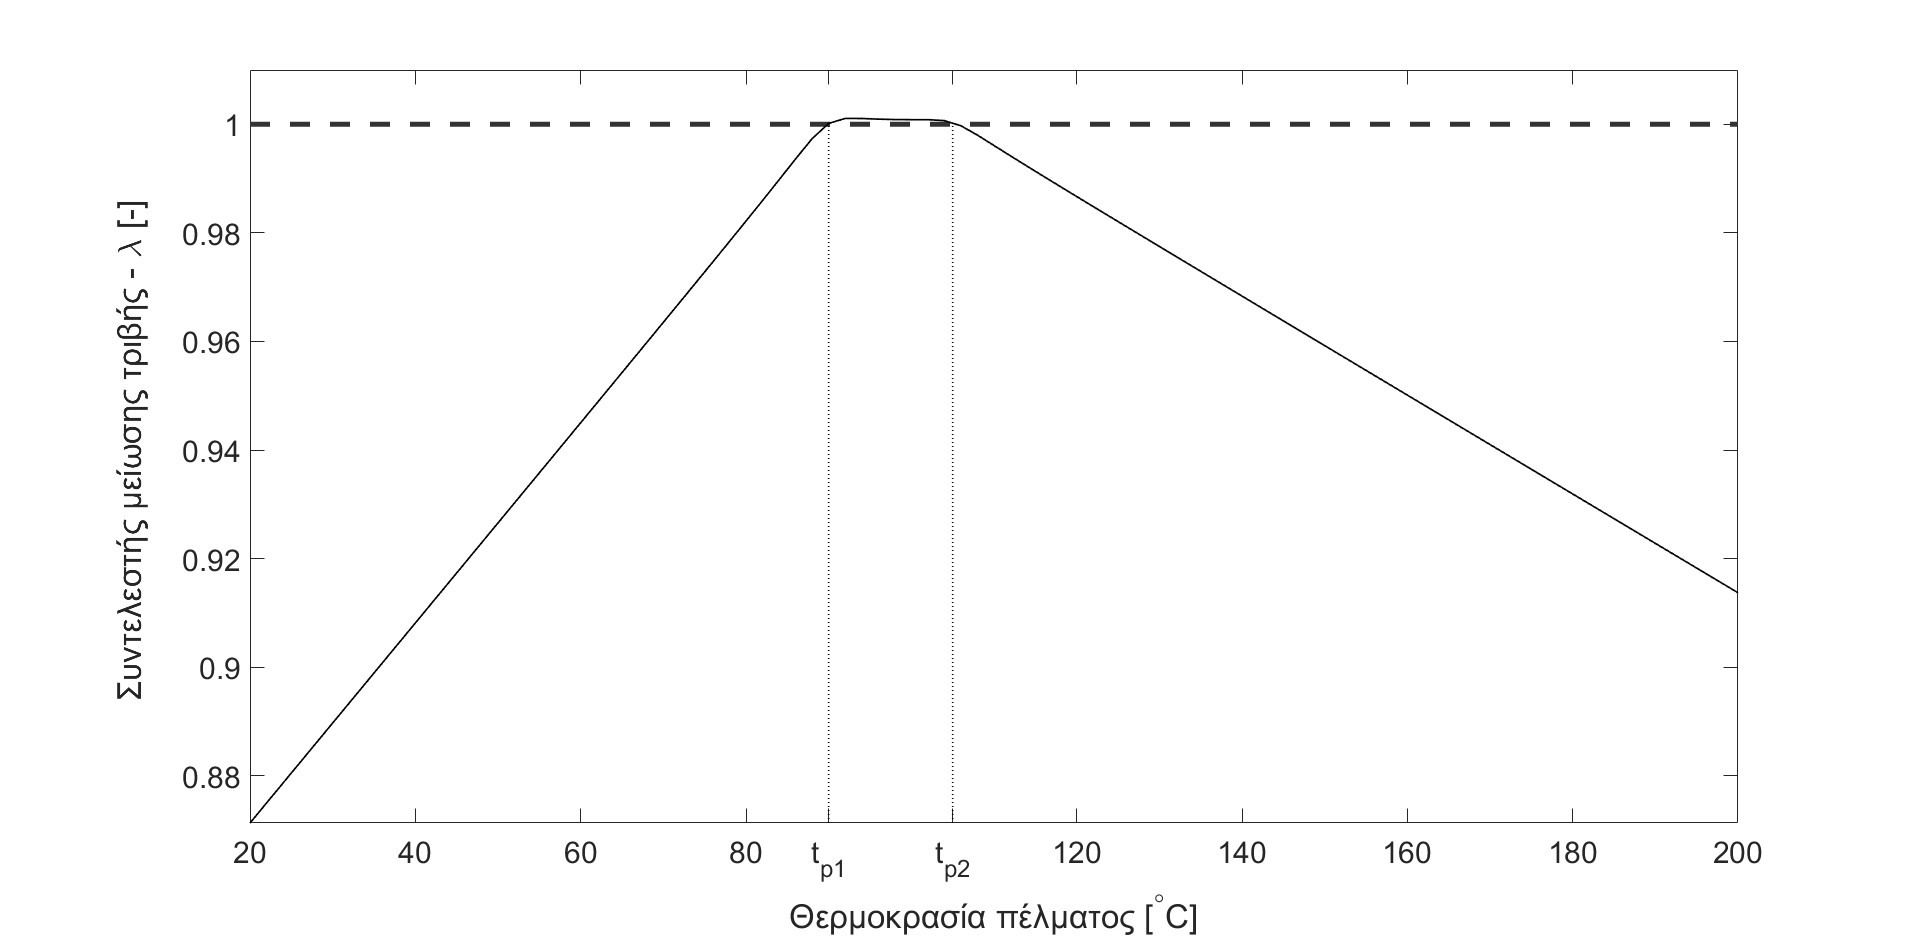
\includegraphics[width=0.8\textwidth]{figures/temp-scaling-factor.jpg}
    \end{center}
    \caption{Συντελεστής μείωσης τριβής συναρτήσει θερμοκρασίας}
    \label{fig:temp-scaling}
\end{figure}

% ------------------------------------------------------------
%  2) Θερμοκρασιακό scaling πρόσφυσης
% ------------------------------------------------------------
\begin{table}[htbp]
    \centering
    \small
    \renewcommand{\arraystretch}{1.2}
    \begin{tabular}{@{}l l l@{}}
        \toprule
        \textbf{Παράμετρος} & \textbf{Τιμή (Μονάδα)} & \textbf{Περιγραφή} \\
        \midrule
        $T_{p1}$              & $90\,^\circ\mathrm{C}$   & Κάτω όριο θερμικού παραθύρου \\
        $T_{p2}$              & $105\,^\circ\mathrm{C}$  & Άνω όριο θερμικού παραθύρου \\
        $\lambda(T_{\text{cold}})$  & $0.908$                  & Συντελεστής μείωσης πρόσφυσης -- $40\,^\circ\mathrm{C}$ \\
        $\lambda(T_{\text{hot}})$   & $0.95$                   & Συντελεστής μείωσης πρόσφυσης -- $160\,^\circ\mathrm{C}$ \\
        $g_{s,\mu}$           & $0.3$                    & Παράμετρος εξομάλυνσης μεταβάσεων του $\lambda(T)$ \\
        \bottomrule
    \end{tabular}
    \caption{Παράμετροι μείωσης πρόσφυσης συναρτήσει της θερμοκρασίας.}
    \label{tab:params_tempscale}
\end{table}

\subsection{Εξάρτηση πρόσφυσης από φθορά}

Ο λόγος μείωσης της πρόσφυσης λόγω φθοράς μοντελοποιείται με ανάλογο εμπειρικό
τρόπο, ακολουθώντας ποιοτικά τη μορφή του σχήματος \ref{fig:tractionVsWear},
χρησιμοποιώντας τέσσερις γραμμικές περιοχές με ομαλές μεταβάσεις.
Ως ανεξάρτητη μεταβλητή χρησιμοποιείται η αδιάστατη φθορά (λόγος φθοράς) που προκύπτει ως $w_{n} = \dfrac{w}{w_{ref}}$, όπου $w_{ref}$ είναι η φθορά αναφοράς, στην πράξη στο επίπεδο φθοράς όπου το ελαστικό δεν μπορεί πλέον να χρησιμοποιηθεί.\\[0.5cm]

Οι επί μέρους ευθείες ορίζονται με βάση τα ζεύγη $w_i, \gamma_i$ των σημείων που ενώνουν. Με τη βοήθειά τους, ορίζουμε ως $\ell_i(w) = a_i w + b_i$ την ευθεία της $i$-οστής περιοχής
($i = 1,\dots,4$), προκύπτει:

\begin{equation}
\begin{aligned}
\gamma(w) = \ell_1(w)
   &+ \Bigl(0.5 + 0.5\sin\bigl(\tan^{-1}(g_s(w - w_{p1}))\bigr)\Bigr)
     \cdot \bigl(\ell_2(w) - \ell_1(w)\bigr) \\[4pt]
   &+ \Bigl(0.5 + 0.5\sin\bigl(\tan^{-1}(g_s(w - w_{p2}))\bigr)\Bigr)
     \cdot \bigl(\ell_3(w) - \ell_2(w)\bigr) \\[4pt]
   &+ \Bigl(0.5 + 0.5\sin\bigl(\tan^{-1}(g_s(w - w_{p3}))\bigr)\Bigr)
     \cdot \bigl(\ell_4(w) - \ell_3(w)\bigr)
\end{aligned}
\label{eq:wearScaleFactor}
\end{equation}

Οι παράμετροι $a_i, b_i$ ($i = 1,\dots,4$) περιγράφουν την κλίση και το σημείο
τομής κάθε γραμμικής περιοχής, οι παράμετροι $w_{p1}, w_{p2}, w_{p3}$
σηματοδοτούν τα σημεία μετάβασης μεταξύ διαδοχικών περιοχών, και η παράμετρος
$g_s$ ελέγχει την ομαλότητα των μεταβάσεων. Με τις τιμές των παραμέτρων που
φαίνονται στον πίνακα \ref{tab:params_wearscale}, η καμπύλη που προκύπτει
φαίνεται στο \cref{fig:wear-scaling}.

\begin{figure}[ht!]
    \begin{center}
        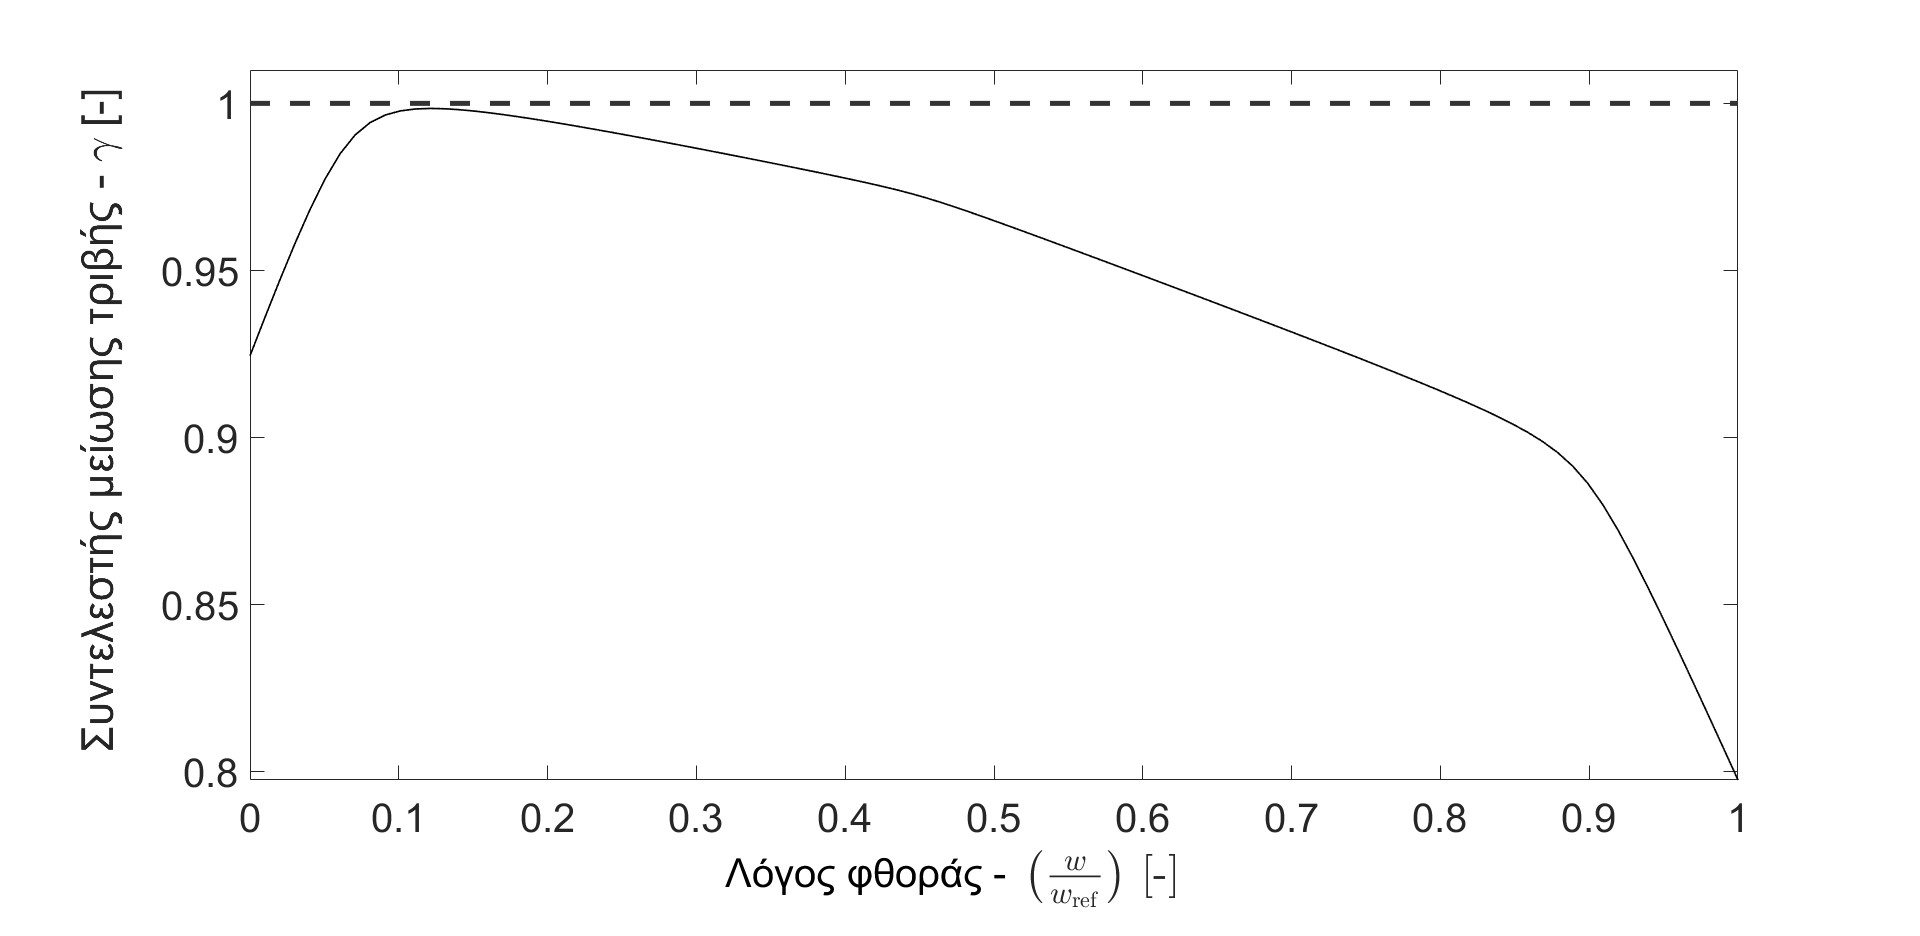
\includegraphics[width=0.8\textwidth]{figures/wear-scaling-factor.jpg}
    \end{center}
    \caption{Συντελεστής μείωσης πρόσφυσης συναρτήσει λόγου φθοράς}
    \label{fig:wear-scaling}
\end{figure}


% ------------------------------------------------------------
%  Παράμετροι scaling πρόσφυσης με φθορά
% ------------------------------------------------------------
\begin{table}[htbp]
    \centering
    \small
    \renewcommand{\arraystretch}{1.2}
    \begin{tabular}{@{}l l l@{}}
        \toprule
        \textbf{Παράμετρος} & \textbf{Τιμή (Μονάδα)} & \textbf{Περιγραφή} \\
        \midrule
        $w_1,\ \gamma_1$  & $0.00,\ 0.93$   & Αρχικό σημείο (αφόρτιστο ελαστικό) \\
        $w_2,\ \gamma_2$  & $0.065,\ 1.00$   & Κορυφή πρόσφυσης μετά το scrubbing-in \\
        $w_3,\ \gamma_3$  & $0.45,\ 0.975$   & Καμπή προς ήπια πτώση \\
        $w_4,\ \gamma_4$  & $0.90,\ 0.90$   & Έναρξη απότομης πτώσης πρόσφυσης \\
        $w_5,\ \gamma_5$  & $1.00,\ 0.80$   & Τελικό σημείο (μέγιστη επιτρεπτή φθορά) \\
        $g_{s,w}$          & $30$            & Παράμετρος εξομάλυνσης μεταβάσεων του $\gamma(w)$ \\
        \bottomrule
    \end{tabular}
    \caption{Παράμετροι μείωσης πρόσφυσης συναρτήσει της φθοράς.}
    \label{tab:params_wearscale}
\end{table}

\subsection{Θερμικό μοντέλο ελαστικού}
% ============================================================
%  §3.2 Θερμικό μοντέλο ελαστικού
% ============================================================

\label{subsec:thermal_model}

Το θερμικό μοντέλο των ελαστικών που αναπτύσσεται στην παρούσα εργασία είναι ένα μοντέλο
συγκεντρωμένων ιδιοτήτων (\textit{lumped}), ενός βαθμού ελευθερίας (θερμοκρασία πέλματος)
και ακολουθεί κατά κύριο λόγο το μοντέλο που αναπτύσσουν οι Tremlett και Limebeer \cite{Tremlett2016}.
Το μοντέλο αυτό θεωρεί πως το πέλμα δε συναλλάσσει θερμότητα με τις γειτονικές του μάζες
και αλληλεπιδρά παρά μόνο μέσω της θερμότητας που παράγεται και απάγεται από το περιβάλλον.
Στην πράξη αυτή η παραδοχή αποτελεί σημαντική απλούστευση της πραγματικότητας: αν αγνοήσουμε
παράπλευρες πηγές ή καταβόθρες θερμότητας, η μάζα του σκελετού δρα ως μία "δεξαμενή" θερμότητας
που σταθεροποιεί τη θερμοκρασία του πέλματος κατά την οδήγηση. Επιπλέον, λόγω της θερμικής
αντίστασης μεταξύ πέλματος και σκελετού του ελαστικού, το πέλμα έχει την ελευθερία να
θερμανθεί παραπάνω από τον σκελετό του ελαστικού στιγμιαία. Επομένως, δε θα ήταν σωστή
η μοντελοποίηση ολόκληρης της μάζας του ελαστικού με μία μεταβλητή κατάστασης καθώς αυτό θα
οδηγούσε σε πολύ υψηλές χρονικές σταθερές -- δηλαδή πολύ αργή απόκριση του πέλματος
σε θερμότητα \cite{West2022}. Η μοντελοποίηση της θερμικής μάζας του σκελετού ως δεύτερης μεταβλητής
κατάστασης αποτελεί την κυριότερη μελλοντική βελτίωση του μοντέλου συγκεντρωμένων ιδιοτήτων.
Στη βιβλιογραφία υπάρχουν επίσης κατανεμημένα θερμικά μοντέλα πεπερασμένων στοιχείων, με κύριο σκοπό
την επιπλέον μοντελοποίηση της κατανομής θερμοκρασίας στο πέλμα \cite{Farroni2014TRT}. \\[0.2cm]

Η επιλογή του απλούστερου μοντέλου είναι σκόπιμη. Η επίλυση ενός συστήματος
δύο Σ.Δ.Ε. εισάγει αμελητέο υπολογιστικό κόστος συγκριτικά με ολόκληρο τον υπολογισμό
της δυναμικής του οχήματος. Ωστόσο, η επιλογή πολυπλοκότερου μοντέλου εισάγει μεγάλο
αριθμό παραμέτρων και φυσικών ιδιοτήτων που αφενός συνεπάγονται μεγαλύτερη ευαισθησία
στο μοντέλο, και αφετέρου χρειάζονται ακόμη μεγαλύτερο σύνολο πειραματικών 
δεδομένων για τον χαρακτηρισμό τους. Χρησιμοποιείται το θερμικό μοντέλο
και οι φυσικές παράμετροι των Tremlett και Limebeer \cite{Tremlett2016} οι οποίοι
επιτυγχάνουν αξιοσημείωτη συσχέτιση με πειραματικά δεδομένα, ακόμη και με απλούστερη
μοντελοποίηση.

\subsubsection{Υπολογισμός θερμότητας}

Στο θερμικό μοντέλο λαμβάνονται υπόψη οι εξής κυρίαρχες μορφές θερμότητας.

\begin{enumerate}
    \item $Q_1$ -- Θερμότητα λόγω τριβής της περιοχής ολίσθησης με το οδόστρωμα
    \item $Q_2$ -- Θερμότητα λόγω υστέρησης του ελαστομερούς
    \item $Q_3$ -- Θερμότητα συναγωγής με περιβάλλοντα αέρα
    \item $Q_4$ -- Θερμότητα αγωγής με οδόστρωμα
\end{enumerate}

\paragraph{Θερμότητα λόγω τριβής.}

Η ισχύς που παράγεται λόγω τριβής της περιοχής ολίσθησης του πέλματος υπολογίζεται ως
άθροισμα των όρων ισχύος του διαμήκους και εγκάρσιου φορτίου.

\begin{equation}
    Q_1 = p_1u_n\bigl(\lvert F_x\kappa\rvert + \lvert F_ytan(\alpha)\rvert\bigr)
    \label{eq:Q1}
\end{equation}

Όπου $\alpha,\kappa$ τα μεγέθη ολίσθησης, $F_x, F_y$ 
η διαμήκης και εγκάρσια δύναμη, $u_n$ η διαμήκης ταχύτητα του ελαστικού, 
και $p_1$ αδιάστατη παράμετρος που διορθώνει για το ποσό θερμότητας που απορροφά
το οδόστρωμα.

\paragraph{Θερμότητα λόγω υστέρησης.}

Η ισχύς που παράγεται λόγω υστέρησης υπολογίζεται ως
άθροισμα των όρων ισχύος που παράγονται λόγω καθενός από τα διαμήκη, εγκάρσια και κατακόρυφα φορτία.

\begin{equation}
    Q_2 = u_n\bigl(p_2\lvert F_x \rvert
    + p_3\lvert F_y \rvert
    + p_4\lvert F_z \rvert
    \bigr)
    \label{eq:Q2}
\end{equation}

Όπου $F_{\{x,y,z\}}$ το διαμήκες, εγκάρσιο και κατακόρυφο φορτίο αντίστοιχα,
και οι παράμετροι $p_{2\dots4}$ εκφράζουν την απόδοση κάθε όρου -- δηλαδή
πόσο η κυκλική παραμόρφωση που παράγει κάθε όρος μεταφράζεται σε θερμότητα.
\paragraph{Θερμότητα συναγωγής.}

Για τη συναγωγή με τον αέρα περιβάλλοντος θερμοκρασίας $T_{\text{περ.}}$ χρησιμοποιείται ένας
Νευτώνειος νόμος ψύξης.

\begin{equation}
    Q_3 = p_5u^{p_6}\bigl(T_s - T_{\text{περ.}}\bigr)
    \label{eq:Q3}
\end{equation}


Όπου $u$ η ταχύτητα του οχήματος και $p_{5,6}$ παράμετροι που εκφράζουν τη διαφορά στη ροή
αέρα που βλέπει ο κάθε τροχός.

\paragraph{Θερμότητα αγωγής με οδόστρωμα.}

Η θερμότητα που άγεται μεταξύ του ελαστικού στην περιοχή προσκόλλησης και το οδόστρωμα δίνεται από

\begin{equation}
    Q_4 = h_tA_{\text{πέλμα}}\bigl(T_s - T_{οδ.}\bigr)
    \label{eq:Q4}
\end{equation}

Όπου $h_t$ ο συντελεστής συναλλαγής θερμότητας στη διεπαφή ελαστικού -- ασφάλτου και $A_{\text{πέλμα}}$
η επιφάνεια επαφής της περιοχής προσκόλλησης του πέλματος.

Για τον προσδιορισμό των φυσικών μεγεθών μπορούν να ακολουθηθούν διάφορες προσεγγίσεις ή μετρήσεις, ωστόσο,
ακολουθούμε το μοντέλο των Tremlett \& Limebeer \cite{Tremlett2016} και τα προσεγγίζουμε με τις 
\cref{eq:contactArea1,eq:contactArea2,eq:contactArea3}.

Η επιφάνεια επαφής του πέλματος θεωρείται ορθογωνική με πλάτος $C_w$ και μήκος $C_l$. Το πλάτος μπορεί 
να διαφέρει μεταξύ των εμπρόσθιων και οπίσθιων τροχών, οπότε το χωρίζουμε σε $C_{wf},C_{wr}$ για πλάτος
των εμπρός και πίσω ελαστικών αντίστοιχα.
Το μήκος της επιφάνειας επαφής του πέλματος δίνεται από την εμπειρική εκθετική σχέση 
(\ref{eq:contactArea1}).
\begin{equation}
    C_l = \alpha_{cp}F_z^{0.7}
    \label{eq:contactArea1}
\end{equation}

Η εμπειρική σταθερά $\alpha_{cp}$ είναι υπεύθυνη για την προσαρμογή σε πραγματικά δεδομένα και την πιθανή διαφοροποίηση
μεταξύ των εμπρόσθιων και οπίσθιων τροχών.

Το μήκος της περιοχής προσκόλλησης $C_{\text{πρ.},l}$ δίνεται από τον λόγο $C_s(\alpha)$ 
που εκφράζει το ποσοστό του μήκους του πέλματος που είναι προσκολλημένο (μη ολισθαίνον), ως $C_{\text{πρ.},l} = C_s\,C_l$. Ο συντελεστής $C_s(\alpha)$
λαμβάνεται από γραμμική παρεμβολή μεταξύ δύο γνωστών καταστάσεων (γωνιών ολίσθησης), ακολουθώντας την εμπειρική προσέγγιση των Tremlett \& Limebeer \cite{Tremlett2016}.

\begin{equation}
    C_s(\alpha) = \dfrac{\alpha}{\alpha_c}(C_{s2}-C_{s1}) + C_{s1}
    \label{eq:contactArea2}
\end{equation}

Επομένως, τελικά το εμβαδό της περιοχής προσκόλλησης του πέλματος, μέσω της οποίας άγεται θερμότητα προς το οδόστρωμα, για εμπρός και πίσω τροχούς δίνεται από

\begin{equation}
    \begin{aligned}
        A_{\text{πέλμα},f} &= C_{wf}C_sC_l\\
        A_{\text{πέλμα},r} &= C_{wr}C_sC_l
    \end{aligned}
    \label{eq:contactArea3}
\end{equation}

\subsubsection{Εξίσωση κατάστασης}

Η θερμική εξίσωση κατάστασης προκύπτει από ισοζύγιο ενέργειας στη μάζα του πέλματος $m_c$.

\begin{equation}
    \frac{dT}{dt} = \frac{Q_1 + Q_2 - Q_3 - Q_4}{m_c \cdot c_{p,c}}
    \label{eq:dTdt_full}
\end{equation}

Εδώ $Q_1, Q_2$ είναι οι πηγές θερμότητας (\cref{eq:Q1,eq:Q2}) και $Q_3, Q_4$ οι απώλειες
(\cref{eq:Q3,eq:Q4}). Στον παρονομαστή η ποσότητα $m_c \cdot c_{p,c}$ εκφράζει τη θερμική
αδράνεια: μεγαλύτερη μάζα σημαίνει βραδύτερη απόκριση.\\[0.5cm]

Οι προσομοιωτές γύρου λειτουργούν σε πεδίο θέσης $s$ (κατά μήκος πίστας) και όχι χρόνου.
Εφαρμόζοντας τον κανόνα αλυσίδας $dt = ds/v$:

\begin{equation}
    \frac{dT}{ds} = \frac{1}{v}\cdot\frac{dT}{dt} = \frac{Q_1 + Q_2 - Q_3 - Q_4}{m_c \cdot c_{p,c} \cdot v}
    \label{eq:dTds_full}
\end{equation}

Αξίζει να παρατηρηθεί η σημασία της διαίρεσης με $v$: σε χαμηλή ταχύτητα,
ακόμα και μικρό $Q_{\rm net}$ οδηγεί σε μεγάλο $dT/ds$ -- γι' αυτό οι αργές στροφές μπορεί
να είναι πιο επιβαρυντικές για το ελαστικό ανά μέτρο πίστας. Αν αυτό συνδυαστεί με στροφή
όπου μπορεί να έχουμε μεγάλη παραγωγή θερμότητας, αυτό ερμηνεύεται φυσικά ως το όχημα να
ξοδεύει περισσότερο χρόνο σε κατάσταση που παράγεται πολλή θερμότητα.

% ------------------------------------------------------------
%  3) Θερμικό μοντέλο (τιμές τροχού FL)
% ------------------------------------------------------------
\begin{table}[htbp]
    \centering
    \small
    \renewcommand{\arraystretch}{1.2}
    \begin{tabular}{@{}l l l@{}}
        \toprule
        \textbf{Παράμετρος} & \textbf{Τιμή (Μονάδα)} & \textbf{Περιγραφή} \\
        \midrule
        $p_1$                & $0.455$                 & Γραμμικός συντελεστής όρου τριβής $Q_1$ \\
        $p_2$                & $1.0 \cdot 10^{-3}$     & Γραμμ. συντ. $F_x$ όρου έργου παραμόρφωσης $Q_2$ \\
        $p_3$                & $1.1 \cdot 10^{-2}$     & Γραμμ. συντ. $F_y$ όρου έργου παραμόρφωσης $Q_2$ \\
        $p_4$                & $2.2 \cdot 10^{-2}$     & Γραμμ. συντ. $F_z$ όρου έργου παραμόρφωσης $Q_2$ \\
        $p_5$                & $1.1 \cdot 10^{-2}$     & Γραμμικός συντελεστής όρου συναγωγής $Q_3$ \\
        $p_6$                & $2.17$                  & Εκθέτης ταχύτητας όρου συναγωγής $Q_3$ \\
        $C_{wf}$               & $0.20$ m                & Πλάτος εμπρόσθιου ελαστικού \\
        $C_{wr}$               & $0.22$ m                & Πλάτος οπίσθιου ελαστικού \\
        $h_t$                & $12$ kW/m$^2$K          & Συντ. αγωγιμότητας πέλματος-οδοστρώματος \\
        $m_c$                & $0.5$ kg                & Ενεργός θερμική μάζα πέλματος \\
        $c_{p,c}$            & $1800$ J/kg K           & Ειδική θερμοχωρητικότητα ελαστομερούς \\
        $\alpha_{cp}$        & $0.056$                & Σταθερά παραμόρφωσης πέλματος με κατακόρυφο φορτίο \\
        $\alpha_c$           & $8^\circ$           & Γωνία ολίσθησης αναφοράς για γραμμ. παρ. \\
        $C_{s1}$             & $0.3$                  & Ποσοστό περιοχής προσκόλλησης -- σημείο 1\\
        $C_{s2}$             & $0.8$                  & Ποσοστό περιοχής προσκόλλησης -- σημείο 2\\
        $T_{\mathrm{amb}}$   & $25\,^\circ\mathrm{C}$  & Θερμοκρασία αέρα περιβάλλοντος \\
        $T_{\mathrm{track}}$ & $35\,^\circ\mathrm{C}$  & Θερμοκρασία επιφάνειας οδοστρώματος \\
        \bottomrule
    \end{tabular}
    \caption{Παράμετροι θερμικού μοντέλου. Παρατίθενται οι τιμές του εμπρόσθιου
    αριστερού τροχού ως ενδεικτικές.}
    \label{tab:params_thermal}
\end{table}

\subsection{Μοντελοποίηση φθοράς}
% ============================================================
%  Μοντέλο φθοράς ελαστικού -- μαθηματική διατύπωση
% ============================================================

\label{subsec:wear_model}

Το μοντέλο φθοράς που χρησιμοποιείται στην παρούσα εργασία ακολουθεί την προσέγγιση των
Tremlett και Limebeer \cite{Tremlett2016}, η οποία με τη σειρά της βασίζεται στη θεωρία των δύο
μηχανισμών τριβής ελαστομερούς και επαληθεύεται απο πειραματικά δεδομένα του Grosch \cite{Grosch2004}. Οι τρεις μακροσκοπικοί μηχανισμοί
φθοράς που περιγράφηκαν στο \cref{subsubsec:graining_blistering} -- τριβολογική
φθορά λόγω ολίσθησης, \textit{graining}, και \textit{blistering} -- μοντελοποιούνται ξεχωριστά και υπερτίθενται.
Η μετάβαση μεταξύ της περιοχής χαμηλής και υψηλής θερμοκρασίας μοντελοποιείται με ομαλή συνάρτηση κατ' ανάλογο τρόπο με
τον συντελεστή μείωσης λόγω θερμοκρασίας. 

\subsubsection{Ρυθμός τριβολογικής φθοράς}

Ο ρυθμός τριβολογικής φθοράς $W_p$ συνδέεται άμεσα με το έργο τριβής ολίσθησης στο
πέλμα. Δεδομένου ότι το έργο αυτό μετατρέπεται σχεδόν εξ ολοκλήρου σε θερμότητα (όρος
$Q_1$ του θερμικού μοντέλου), ο ρυθμός φθοράς εκφράζεται μέσω μιας
εκθετικής σχέσης \cite{Grosch2004}:

\begin{equation}
    \dot{w}_p = \dot{w}_{p1} \cdot \left(\frac{Q_1}{Q_{\mathrm{ref}}}\right)^{W_{p2}}
    \label{eq:w_p}
\end{equation}

όπου $Q_{\mathrm{ref}}$ ισχύς αναφοράς στην οποία έγινε η μέτρηση, $\dot{w}_{p1}$ ο ρυθμός φθοράς σε συνθήκες αναφοράς
και $\dot{w}_{p2}$ εκθέτης που ρυθμίζει τη μη γραμμικότητα της απόκρισης. Για $\dot{w}_{p2} > 1$ η
φθορά επιταχύνεται δυσανάλογα σε συνθήκες υψηλής ολίσθησης, γεγονός που επιβεβαιώνεται με
πειραματικές παρατηρήσεις \cite{Grosch2004,Tremlett2016}.

\subsubsection{Ρυθμός graining}

Ο ρυθμός graining $\dot{w}_g$ ενεργοποιείται όταν η θερμοκρασία πέλματος πέφτει κάτω από την
κρίσιμη θερμοκρασία μετάβασης $T_{\mathrm{tp}}$ και μηδενίζεται πάνω από αυτήν.
Μοντελοποιείται με εμπειρική σχέση και παραμέτρους προς διερεύνηση.

\begin{equation}
    \dot{w}_g = W_{g1} \cdot (t_{\mathrm{tp}} - T)^{W_{g2}}
    \label{eq:w_g}
\end{equation}

όπου ο εκθέτης $W_{g2}$ παίζει το ρόλο της επιτάχυνσης της φθοράς μη γραμμικά με τη θερμοκρασία, και ο συντελεστής $W_{g1}$ ελέγχει τη συνολική επίδραση του 
\textit{graining}.

\subsubsection{Ρυθμός blistering}

Αντίστοιχα, ο ρυθμός blistering $\dot{w}_b$ ενεργοποιείται πάνω από την κρίσιμη θερμοκρασία και
μηδενίζεται κάτω από αυτήν. Κατ'αντιστοιχία, ελέγχεται από δύο παραμέτρους, $W_{b1}$ που
καθορίζει την κλίμακα και $W_{b2}$ που ελέγχει την ένταση της εξάρτησης από τη θερμοκρασία.

\begin{equation}
    \dot{w}_b = W_{b1} \cdot (T - t_{\mathrm{tp}})^{W_{b2}}
    \label{eq:Wb}
\end{equation}

Η επιλογή κοινής κρίσιμης θερμοκρασίας $t_{\mathrm{tp}}$ και για τους δύο μηχανισμούς
graining και blistering είναι απλοποίηση: στην πραγματικότητα το θερμικό παράθυρο έχει
μικρό εύρος και όχι μηδενικό, αλλά η επιλογή αυτή διατηρεί τη μαθηματική συμμετρία του
μοντέλου και τεκμηριώνεται στη βιβλιογραφία \cite{West2022,Tremlett2016}.

\subsubsection{Συνολικός ρυθμός φθοράς}

Ο συνολικός ρυθμός φθοράς προκύπτει από την υπέρθεση των τριών μηχανισμών, με ομαλή
μετάβαση στη βέλτιστη θερμοκρασία $t_{tp}$.

\begin{equation}
\dot{w_a}(T_s,Q_1) = (\dot{w}_g+\dot{w}_p) + \Bigl(0.5+0.5sin\bigl(tan^{-1}\bigl(g_s(T_s-t_{tp})\bigr)\bigr)\Bigr)
\cdot \Bigl(\bigl(\dot{w}_b +\dot{w}_p \bigr) -
\bigl(\dot{w}_g +\dot{w}_p \bigr) \Bigr)
    \label{eq:Wtotal}
\end{equation}

Η παράμετρος $g_s$ -- κοινή σε όλες τις ομαλές συναρτήσεις -- ρυθμίζει την καμπυλότητα της μετάβασης:
μικρές τιμές δίνουν ομαλή μετάβαση ενώ όσο αυξάνεται η τιμή της, η τελική μορφή της καμπύλης προσεγγίζει τμηματική συνάρτηση των δύο καμπυλών.

\subsubsection{Ολοκλήρωση σε συσσωρευμένη φθορά}

Ο ρυθμός φθοράς $\dot{w_a}$ έχει διαστάσεις μήκους ανά χρόνο (πάχος πέλματος που χάνεται ανά
δευτερόλεπτο). Η συσσωρευμένη φθορά κατά τη διάρκεια ενός γύρου προκύπτει από
ολοκλήρωση κατά μήκος της τροχιάς, χρησιμοποιώντας τον κανόνα αλυσίδας για μετατροπή από
τη χρονική στη χωρική ανεξάρτητη μεταβλητή:

\begin{equation}
    \frac{dw_a}{ds} = \frac{1}{v}\, \dot{w}_a(T, Q_1)
    \label{eq:dwds}
\end{equation}

με $v$ την ταχύτητα του οχήματος.


Στον παρακάτω πίνακα (\ref{tab:params_wear}) παρατίθενται ενδεικτικές τιμές των παραμέτρων του μοντέλου φθοράς.

\begin{table}[htbp]
    \centering
    \small
    \renewcommand{\arraystretch}{1.2}
    \begin{tabular}{@{}l l l@{}}
        \toprule
        \textbf{Παράμετρος} & \textbf{Τιμή (Μονάδα)} & \textbf{Περιγραφή} \\
        \midrule
        $W_{p1}$             & $0.09$ mm/s                 & Ρυθμός φθοράς ολίσθησης στην ισχύ αναφοράς \\
        $W_{p2}$             & $1.6$                       & Εκθέτης μη γραμμικότητας φθοράς ολίσθησης \\
        $Q_{\mathrm{ref}}$   & $150$ kW                    & Ισχύς αναφοράς όρου φθοράς ολίσθησης\\
        $W_{g1}$             & $4 \cdot 10^{-6}$ mm/K$^2$s & Συντελεστής έντασης graining \\
        $W_{g2}$             & $2$                         & Εκθέτης θερμοκρασιακής εξάρτησης graining \\
        $W_{b1}$             & $8 \cdot 10^{-6}$ mm/K$^2$s & Συντελεστής έντασης blistering \\
        $W_{b2}$             & $2$                         & Εκθέτης θερμοκρασιακής εξάρτησης blistering \\
        $T_{\mathrm{tp}}$    & $100\,^\circ\mathrm{C}$     & Βέλτιστη θερμοκρασία -- μετάβαση graining-blistering \\
        \bottomrule
    \end{tabular}
    \caption{Παράμετροι μοντέλου φθοράς.}
    \label{tab:params_wear}
\end{table}

\subsection{Συγκεντρωτικοί πίνακες παραμέτρων}
\label{subsec:tyre_params_table}
% ============================================================
%  Συγκεντρωτικοί πίνακες παραμέτρων του μοντέλου ελαστικού
%  (τέσσερις λειτουργικά διαχωρισμένοι πίνακες)
% ============================================================

Στους παρακάτω πίνακες παρατίθενται οι παράμετροι του μοντέλου ελαστικού που
αναπτύχθηκε, ομαδοποιημένες κατά υπομοντέλο: συνδυαστική πρόσφυση
(\cref{tab:params_combined}), θερμοκρασιακό scaling πρόσφυσης
(\cref{tab:params_tempscale}), θερμικό μοντέλο (\cref{tab:params_thermal}) και
μοντέλο φθοράς (\cref{tab:params_wear}). Οι τιμές αντιστοιχούν στη βαθμονόμηση
που χρησιμοποιήθηκε στις προσομοιώσεις της παρούσας εργασίας.





% ------------------------------------------------------------
%  4) Μοντέλο φθοράς
% ------------------------------------------------------------
\begin{table}[htbp]
    \centering
    \small
    \renewcommand{\arraystretch}{1.2}
    \begin{tabular}{@{}l l l@{}}
        \toprule
        \textbf{Παράμετρος} & \textbf{Τιμή (Μονάδα)} & \textbf{Περιγραφή} \\
        \midrule
        $W_{p1}$             & $0.09$ mm/s                 & Ρυθμός τριβολογικής φθοράς στην ισχύ αναφοράς \\
        $W_{p2}$             & $1.6$                       & Εκθέτης μη γραμμικότητας τριβολογικής φθοράς \\
        $Q_{\mathrm{ref}}$   & $150$ kW                    & Ισχύς αναφοράς όρου τριβολογικής φθοράς \\
        $W_{g1}$             & $4 \cdot 10^{-6}$ mm/K$^2$s & Συντελεστής έντασης graining \\
        $W_{g2}$             & $2$                         & Εκθέτης θερμοκρασιακής εξάρτησης graining \\
        $W_{b1}$             & $8 \cdot 10^{-6}$ mm/K$^2$s & Συντελεστής έντασης blistering \\
        $W_{b2}$             & $2$                         & Εκθέτης θερμοκρασιακής εξάρτησης blistering \\
        $T_{\mathrm{tp}}$    & $100\,^\circ\mathrm{C}$     & Κρίσιμη θερμοκρασία μετάβασης graining-blistering \\
        $g_{s,W}$            & $0.3$                       & Οξύτητα σιγμοειδούς μετάβασης μοντέλου φθοράς \\
        \bottomrule
    \end{tabular}
    \caption{Παράμετροι μοντέλου φθοράς.}
    \label{tab:params_wear}
\end{table}


\clearoddpage
\section{Μοντέλο Οχήματος}
\label{sec:vehicle_model}
\documentclass[../main.tex]{subfiles}
\begin{document}

% ============================================================
%  §4.1 Μοντέλο Οχήματος -- δίτροχο μοντέλο, συντεταγμένες, weight transfer
%  Ενσωματωμένα TikZ σχήματα inline.
% ============================================================

\label{sec:vehiclemodel}

Η ενσωμάτωση του μοντέλου ελαστικών σε έναν προσομοιωτή γύρου απαιτεί τον ορισμό ενός μοντέλου οχήματος που να συνδέει τα κινηματικά μεγέθη (ταχύτητα, επιτάχυνση) με τις δυνάμεις που αναπτύσσονται σε κάθε τροχό. Στην παρούσα εργασία χρησιμοποιείται ένα \emph{δίτροχο μοντέλο} (two-track model) τριών βαθμών ελευθερίας: διαμήκης επιτάχυνση, πλευρική επιτάχυνση και στρέψη (yaw). Το μοντέλο αντιμετωπίζει το σώμα ως άκαμπτο σώμα (rigid body) χωρίς δυναμική ανάρτησης -- οι κατακόρυφες μετατοπίσεις μοντελοποιούνται μόνο μέσω της στατικής κατανομής φορτίου.

Η επιλογή δίτροχου έναντι μονότροχου (bicycle model) μοντέλου είναι εδώ αναγκαία: στο δίτροχο διακρίνονται οι αριστεροί από τους δεξιούς τροχούς, γεγονός κρίσιμο για τον υπολογισμό της πλευρικής μεταφοράς φορτίου και για την ανεξάρτητη παρακολούθηση της θερμοκρασίας κάθε τροχού.

% ---
\subsection{Συστήματα συντεταγμένων}
\label{subsec:frames}
% ---

Για τη μαθηματική περιγραφή της κίνησης χρησιμοποιούνται τρία αλληλοεξαρτώμενα συστήματα συντεταγμένων, τα οποία ορίζονται σύμφωνα με τις συμβάσεις SAE \cite{Milliken1995}. Στο \cref{fig:twotrack_topview} φαίνεται η γεωμετρική σχέση τους.

% ----- TikZ: κάτοψη δίτροχου μοντέλου -----
\begin{figure}[htbp]
\centering
\begin{tikzpicture}[scale=1.05,
    wheel/.style={rectangle, draw=black, fill=gray!30,
                  minimum width=0.28cm, minimum height=0.72cm, rounded corners=1pt},
    frameaxis/.style={->, thick},
    carframe/.style={->, thick, red!70!black},
    tyreframe/.style={->, thick, green!50!black},
    dim/.style={<->, thin, gray}
]
  % -- car body --
  \draw[fill=gray!15, draw=black, rounded corners=3pt] (-1.0,-0.55) rectangle (1.0,0.55);
  \node[font=\scriptsize] at (0,0) {Σώμα / CG};

  % -- wheels --
  \node[wheel] (FL) at (-0.65, 0.85) {};  \node[font=\scriptsize,above=1pt] at (FL.north) {FL};
  \node[wheel] (FR) at (-0.65,-0.85) {};  \node[font=\scriptsize,below=1pt] at (FR.south) {FR};
  \node[wheel] (RL) at ( 0.65, 0.85) {};  \node[font=\scriptsize,above=1pt] at (RL.north) {RL};
  \node[wheel] (RR) at ( 0.65,-0.85) {};  \node[font=\scriptsize,below=1pt] at (RR.south) {RR};

  % -- global frame (bottom-left) --
  \begin{scope}[shift={(-2.8,-1.7)}]
    \draw[frameaxis,black] (0,0)--(0.85,0) node[right,font=\small]{$X$};
    \draw[frameaxis,black] (0,0)--(0,0.85) node[above,font=\small]{$Y$};
    \node[font=\scriptsize,below left] at (0,0) {Global};
  \end{scope}

  % -- car frame (rotated β=10°) --
  \begin{scope}[rotate=10]
    \draw[carframe] (0,0)--(0.72,0) node[right,font=\scriptsize,red!70!black]{$x$};
    \draw[carframe] (0,0)--(0,0.72) node[above,font=\scriptsize,red!70!black]{$y$};
  \end{scope}
  \node[font=\scriptsize,red!70!black] at (0.55,0.55) {Car frame};
  % beta arc
  \draw[->,thin,purple] (0.42,0) arc[start angle=0,end angle=10,radius=0.42];
  \node[font=\scriptsize,purple] at (0.68,0.12) {$\beta$};

  % -- tyre frame front (δ=20°) --
  \begin{scope}[shift={(-0.65,0.85)},rotate=20]
    \draw[tyreframe] (0,0)--(0.35,0);
  \end{scope}
  \draw[->,thin,green!50!black] (-0.65+0.22,0.85) arc[start angle=0,end angle=20,radius=0.22];
  \node[font=\scriptsize,green!50!black] at (-0.15,1.12) {$\delta$};

  % -- velocity vector --
  \draw[->,ultra thick,orange!80!black] (0,0)--(-0.55,0.22)
    node[left,font=\small,orange!80!black]{$\mathbf{v}$};

  % -- dimensions --
  \draw[dim] (-0.65,1.2)--(0.65,1.2);
  \node[gray,font=\scriptsize,above] at (0,1.2) {$L$};
  \draw[dim] (-1.1,0.85)--(-1.1,-0.85);
  \node[gray,font=\scriptsize,left] at (-1.1,0) {$t$};

  % -- CG dot --
  \filldraw[black] (0,0) circle (2pt);
\end{tikzpicture}
\caption{Κάτοψη δίτροχου μοντέλου. Αδρανειακό σύστημα (μαύρο), σύστημα σώματος (κόκκινο) υπό γωνία πλαϊνής ολίσθησης $\beta$, γωνία διεύθυνσης εμπρός τροχού $\delta$ (πράσινο) και διάνυσμα ταχύτητας $\mathbf{v}$ (πορτοκαλί).}
\label{fig:twotrack_topview}
\end{figure}
% ----- τέλος TikZ -----

Το \emph{αδρανειακό (global) σύστημα} έχει άξονα $X$ προς τα εμπρός και $Y$ προς τα αριστερά. Στο πλαίσιο αυτό ορίζονται οι μετρούμενες επιταχύνσεις $a_x$ (διαμήκης) και $a_y$ (πλευρική) και ισχύει η εξίσωση ισορροπίας $m\mathbf{a} = \sum_i \mathbf{F}_i$.

Το \emph{σύστημα σώματος (car frame)} είναι σταθερό ως προς το αμάξωμα και περιστρέφεται από το global κατά τη γωνία πλαϊνής ολίσθησης $\beta$ (chassis side-slip angle). Η γωνία $\beta$ εκφράζει την απόκλιση της κατεύθυνσης κίνησης του CG από τον άξονα του οχήματος -- στη συνήθη οδήγηση είναι μικρή ($<5°$), αλλά σε έντονες μανούβρες μπορεί να φτάσει έως $\pm 15°$.

Το \emph{σύστημα τύπου (tyre frame)} χρησιμοποιείται ξεχωριστά για κάθε τροχό. Για τους πίσω τροχούς ταυτίζεται με το car frame. Για τους εμπρός τροχούς περιστρέφεται επιπλέον κατά τη γωνία διεύθυνσης $\delta$ -- στο πλαίσιο αυτό ορίζονται οι δυνάμεις $F_x$ (διαμήκης) και $F_y$ (πλευρική) που αναπτύσσει κάθε τροχός.

% ---
\subsection{Κατανομή κατακόρυφων φορτίων -- Μεταφορά φορτίου}
\label{subsec:weight_transfer}
% ---

Ο κατακόρυφος φόρτος κάθε τροχού καθορίζει άμεσα το μέγιστο εφαπτομενικό που μπορεί να αναπτυχθεί (μέσω του $\mu \cdot F_z$) και την αναλογία θερμότητας που παράγεται ($Q_2 \propto F_z$). Η κατανομή των κατακόρυφων φορτίων αλλάζει δυναμικά με τις επιταχύνσεις.

% ----- TikZ: weight transfer -----
\begin{figure}[htbp]
\centering
\begin{tikzpicture}[scale=0.88,
    vec/.style={->,very thick},
    dim/.style={<->,thin,gray}
]
  % ground
  \draw[thick,gray] (-3.4,0)--(3.4,0);
  \fill[gray!20] (-3.4,-0.15) rectangle (3.4,0);

  % wheels (side view)
  \filldraw[gray!40,draw=black] (-2.1,0.28) circle (0.28);
  \filldraw[gray!40,draw=black] ( 2.1,0.28) circle (0.28);

  % body
  \draw[fill=gray!15,draw=black,rounded corners=3pt] (-2.3,0.56) rectangle (2.3,1.16);
  \node[font=\small] at (0,0.86) {Σώμα};

  % CG
  \filldraw[red] (-0.3,1.16) circle (3pt);
  \node[font=\small,above,red] at (-0.3,1.2) {CG};
  \draw[dashed,gray!60] (-0.3,0.56)--(-0.3,1.6);

  % hCG
  \draw[dim] (-3.0,0.56)--(-3.0,1.16);
  \node[gray,font=\small,left] at (-3.0,0.86) {$h_{\rm CG}$};

  % ax arrow
  \draw[vec,orange!80!black] (-0.3,1.7)--(1.3,1.7)
    node[right,font=\small]{$a_x>0$};

  % Fz arrows (static + delta)
  \draw[vec,blue!70] (-2.1,0.56)--(-2.1,-0.7) node[below,font=\small,blue!70]{$F_{z,f}^{\rm stat}$};
  \draw[vec,blue!70] ( 2.1,0.56)--( 2.1,-0.9) node[below,font=\small,blue!70]{$F_{z,r}^{\rm stat}$};

  % delta Fz
  \draw[vec,red!70,dashed] (-2.1,-0.45)--(-2.1,-0.1);
  \node[font=\scriptsize,red!70,left] at (-2.1,-0.28) {$-\Delta F_z$};
  \draw[vec,red!70,dashed] (2.1,-0.45)--(2.1,-0.9);
  \node[font=\scriptsize,red!70,right] at (2.1,-0.67) {$+\Delta F_z$};

  % wheelbase
  \draw[dim] (-2.1,-1.3)--(2.1,-1.3);
  \node[gray,font=\small,below] at (0,-1.3) {$L$};

  % equation
  \node[font=\small] at (0,-1.9)
    {$\Delta F_{z} = \dfrac{m\,a_x\,h_{\rm CG}}{L}$};
\end{tikzpicture}
\caption{Διαμήκης μεταφορά φορτίου κατά επιτάχυνση ($a_x>0$). Ο εμπρός άξονας αποφορτίζεται κατά $\Delta F_z$ και ο πίσω επιφορτίζεται αντίστοιχα.}
\label{fig:weight_transfer}
\end{figure}
% ----- τέλος TikZ -----

\paragraph{Διαμήκης μεταφορά:}
\begin{equation}
    \Delta F_{z,\text{long}} = \frac{m \cdot a_x \cdot h_{\text{CG}}}{L}
    \label{eq:Fz_long}
\end{equation}

Κατά επιτάχυνση ($a_x > 0$) το φορτίο μεταφέρεται από τον εμπρός στον πίσω άξονα. Κατά φρένα­ρισμα ($a_x < 0$) το αντίθετο -- ο εμπρός άξονας φορτίζεται περισσότερο, γι' αυτό και τα εμπρός ελαστικά υφίστανται εντονότερη φθορά φρεναρίσματος.

\paragraph{Πλευρική μεταφορά:}
\begin{equation}
    \Delta F_{z,\text{lat}} = \frac{m \cdot a_y \cdot h_{\text{CG}}}{t}
    \label{eq:Fz_lat}
\end{equation}

όπου $t$ ο τροχόδρομος (track width) του αντίστοιχου άξονα. Σε δεξιά στροφή ($a_y < 0$ στη σύμβαση $Y$-αριστερά) ο εξωτερικός (αριστερός) τροχός επιφορτίζεται. Αυτή η ασυμμετρία εξηγεί γιατί σε πίστες με κυριαρχία δεξιών στροφών (π.χ. Βαρκελώνη) τα αριστερά ελαστικά θερμαίνονται πιο έντονα.

% TODO: Αν χρησιμοποιείς roll stiffness distribution (anti-roll bars) για το
% πραγματικό split εμπρός/πίσω, αναφέρτο εδώ. Επίσης αξίζει σημείωση για
% aerodynamic downforce: αν το μοντέλο το συμπεριλαμβάνει ως συνάρτηση v².

% ---
\subsection{Επίλυση κατάστασης οχήματος}
\label{subsec:car_state_solver}
% ---

Σε κάθε σημείο $s_k$ της πίστας, γνωρίζουμε $v_k$, $a_{x,k}$ και $a_{y,k}$ (από το προφίλ ταχύτητας και ακτίνα καμπυλότητας, §\ref{subsec:slip_estimation}). Οι δύο άγνωστες ποσότητες που χαρακτηρίζουν την κατάσταση του οχήματος είναι η γωνία διεύθυνσης $\delta$ και η γωνία πλαϊνής ολίσθησης $\beta$.

Η ισορροπία δυνάμεων στο αδρανειακό πλαίσιο απαιτεί:
\begin{equation}
    \sum_{i \in \{FL,FR,RL,RR\}} \mathbf{F}_{i,\text{global}}(\delta,\beta) = m \cdot \mathbf{a}
    \label{eq:force_balance}
\end{equation}

Αυτό αποτελεί σύστημα 2 εξισώσεων (X-Y) με 2 αγνώστους, το οποίο επιλύεται αριθμητικά μέσω \texttt{lsqnonlin} (Newton-Raphson based) με φυσικά όρια $\delta \in [-45°, 45°]$, $\beta \in [-15°, 15°]$. Εσωτερικά, κάθε αξιολόγηση του residual περιλαμβάνει αλυσίδα υπολογισμών: μετασχηματισμοί συντεταγμένων $\to$ κατανομή $F_z$ $\to$ ταχύτητες τροχών $\to$ slip $\to$ δυνάμεις ελαστικού $\to$ global frame.

\end{document}

\clearoddpage
\section{Εκτίμηση μεταβλητών κατάστασης οχήματος}
\label{sec:inverseModel}
\subsection{Εισαγωγή -- επίλυση κατάστασης οχήματος}
Από τις εξισώσεις του κεφαλαίου \ref{sec:tyre_model} είναι εμφανές πως για τον υπολογισμό θερμοκρασίας και φθοράς στα ελαστικά,
είναι απαραίτητο να γνωρίζουμε τα μεγέθη ολίσθησης καθώς και τα φορτία στους τροχούς.
Ένα υπολογιστικό μοντέλο δεν μπορεί να είναι πιο ακριβές απ' ό,τι τα δεδομένα εισόδου του, επομένως η καλύτερη προσέγγιση θα ήταν η απ'ευθείας
μέτρηση των μεγεθών ολίσθησης και φορτίων στα ελαστικά. Ωστόσο, οι αισθητήρες μέτρησης ταχυτήτων στους τροχούς (π.χ. αισθητήρες doppler) συνοδεύονται από πολύ υψηλό κόστος, ενώ
η μέτρηση των φορτίων στους τροχούς είναι σχεδόν αδύνατη ή καθόλου πρακτική. Τέλος, σε συνθήκες αγώνα, οι περισσότεροι αισθητήρες αφαιρούνται από το όχημα, αφενός για τη μείωση του βάρους αλλά αφετέρου
και για την ελαχιστοποίηση των εξαρτημάτων που μπορούν να αστοχήσουν κατά τη διάρκεια του αγώνα.\\
\noindent
Είναι φανερό, λοιπόν, πως χρειάζεται μια μέθοδος προσέγγισης αυτών των μεγεθών χωρίς την απ'ευθείας μέτρησή τους. Για τον λόγο αυτό αναπτύσσεται μια μεθοδολογία
εκτίμησης της καθολικής κατάστασης του οχήματος με τα ελάχιστα δεδομένα εισόδου, η οποία λειτουργεί ουσιαστικά ως ψηφιακό δίδυμο του οχήματος.\\[5pt]

Για την εφαρμογή της παρούσας εργασίας, θεωρείται πως είναι γνωστή η ταχύτητα του οχήματος σε κάθε σημείο κατά μήκος της πίστας ενώ επίσης η τροχιά του οχήματος (γεωμετρία της πίστας). Επιπλέον αισθητήρες, όπως για παράδειγμα επιταχυνσιόμετρο στο κέντρο μάζας, μπορούν να αντικαταστήσουν κάποιο βήμα της διαδικασίας αυξάνοντας την ακρίβεια του εκάστοτε τμήματος.
Τέλος, περαιτέρω μεγέθη που χρησιμοποιούνται στη μοντελοποίηση για την εκτίμηση της κατάστασης θεωρούνται γνωστά και σταθερά χαρακτηριστικά του οχήματος που μπορούν να προσδιορισθούν εκ των προτέρων σε εργαστηριακές δοκιμές. 

Η διαδικασία εκτίμησης, παρουσιάζεται σχηματικά στο \cref{fig:slip_est_flow},
και βασίζεται στην αντίστροφη επίλυση του προβλήματος δυναμικής οχήματος. Η επίλυση επιτυγχάνεται αριθμητικά και αναλύεται σε επόμενη παράγραφο.\\
\noindent
Από τις εισόδους του μοντέλου και τις παραδοχές, μπορούν να εκτιμηθούν ή να μετρηθούν οι ταχύτητες του κέντρου μάζας του οχήματος, και οι αντίστοιχες επιταχύνσεις.\\

Όπως θα αναλυθεί στις επόμενες παραγράφους, καταλήγουμε σε δύο ανεξάρτητες μεταβλητές, τη γωνία πλευρικής ολίσθησης $\beta$, και τη γωνία διεύθυνσης των εμπρόσθιων τροχών $\delta$.

% ----- TikZ: high-level slip estimation pipeline -----
\begin{figure}[htbp]
\centering
\begin{tikzpicture}[
    node distance=0.55cm and 1.0cm,
    block/.style   ={rectangle, draw=black, fill=white,      text width=7cm,
                     align=center, rounded corners=4pt, minimum height=0.9cm, font=\small},
    io/.style      ={rectangle, draw=black, fill=black!5,    text width=5.2cm,
                     align=center, rounded corners=2pt, minimum height=0.9cm, font=\small},
    outbox/.style  ={rectangle, draw=black, fill=black!12,   text width=5.2cm,
                     align=center, rounded corners=2pt, minimum height=0.9cm, font=\small\bfseries},
    decision/.style={diamond,   draw=black, fill=white,      text width=2.4cm,
                     align=center, font=\scriptsize, inner sep=1pt},
    arr/.style     ={->, thick, black}
]

  \node[io]                       (inp)    {Είσοδοι: γεωμετρία πίστας, χρονοσειρά ταχύτητας};
  \node[block, below=of inp]   (kinem)  {Υπολογισμός επιταχύνσεων οχήματος $a_X, a_Y$};
  \node[block, below=of kinem]    (startOfIteration)     {Αρχικοποίηση πλευρικής ολίσθησης\\ και γωνίας τιμονιού ($\beta_0, \delta_0$)};
  \node[block, below=of startOfIteration]    (fz)     {Υπολογισμός κατακόρυφων\\ φορτίων ανά τροχό $F_{z,i}$};
  \node[block, below=of fz]    (wheelSlips)     {Υπολογισμός ταχυτήτων και\\ μεγεθών ολίσθησης τροχών $\alpha_i,\kappa_i$};
  \node[block, below=of wheelSlips]    (tyreForces)     {Υπολογισμός πρόσφυσης\\ ελαστικών $F_{u,i}, F_{v,i}$};
  \node[block, below=of tyreForces]       (solve)  {Επίλυση εξισώσεων ισορροπίας\\ (μόνιμη κατάσταση)};
  \node[decision, below=of solve] (conv)   {σύγκλιση;};
  \node[outbox, below=of conv]    (out)    {Έξοδος: ολισθήσεις και δυνάμεις ανά τροχό ($\alpha_i, \kappa_i, F_{u,i}, F_{v,i}$)};

  \draw[arr] (inp)    -- (kinem);
  \draw[arr] (kinem)  -- (startOfIteration);
  \draw[arr] (startOfIteration)     -- (fz);
  \draw[arr] (fz)  -- (wheelSlips);
  \draw[arr] (wheelSlips)     -- (tyreForces);
  \draw[arr] (tyreForces)     -- (solve);
  \draw[arr] (solve)     -- (conv);
  \draw[arr] (conv)   -- node[right, font=\scriptsize]{ναι} (out);

  % failure branch
  \node[font=\scriptsize, right=0.8cm of conv, align=center]
    (fail) {επισήμανση\\ασύγκλιτου σημείου};
  \draw[arr, dashed] (conv.east) -- (fail.west)
      node[midway, above, font=\scriptsize]{όχι};
      
        % ----- dashed box around the iteration loop -----
  \node[draw=black, dashed, rounded corners=6pt,
        inner sep=8pt, fit=(wheelSlips)(fz)(tyreForces)(solve)] 
        (loopbox) {};
        
  \node[anchor=south, font=\normalsize, xshift=-4pt, rotate=90] 
      at (loopbox.west) {Επαναληπτική διαδικασία};

\end{tikzpicture}
\caption{Διάγραμμα ροής -- εκτίμηση ολισθήσεων και δυνάμεων ανά τροχό από δεδομένα γύρου.}
\label{fig:slip_est_flow}
\end{figure}
% ----- τέλος flowchart -----

\label{subsec:stateSolverIntro}
\subsection{Υπολογισμός κινηματικών μεγεθών}
\label{subsec:stateSolverVelocities}
Ξεκινώντας με την επίλυση της κατάστασης του οχήματος, αξιοποιούμε τα δεδομένα ταχύτητας $U_{\hat{X}}(s)$ του οχήματος σε συνδυασμό με τη γεωμετρία της πίστας.

Οι επιταχύνσεις και ο ρυθμός εκτροπής μετρώνται με επιταχυνσιόμετρα και γυροσκόπια αντίστοιχα καθώς αποτελούν προσιτό πακέτο αισθητήρων με τα οποία είναι εξοπλισμένα πλέον τα περισσότερα αγωνιστικά οχήματα. Ωστόσο, στην παρούσα εργασία θα προσεγγίσουμε αυτά τα μεγέθη μέσω της τροχιάς του οχήματος.\\[5pt]

Η τροχιά του οχήματος εκφράζεται με καμπυλόγραμμες συντεταγμένες (curvilinear), όπου η πίστα αποτυπώνεται ως μία αλληλουχία καμπών σταθερής ακτίνας ή ευθειών (\cref{fig:barcelonaCurvilinear}), σχηματίζοντας τελικά μία περιγραφή της μορφής $R(s)$.

\begin{figure}[ht!]
    \begin{center}
        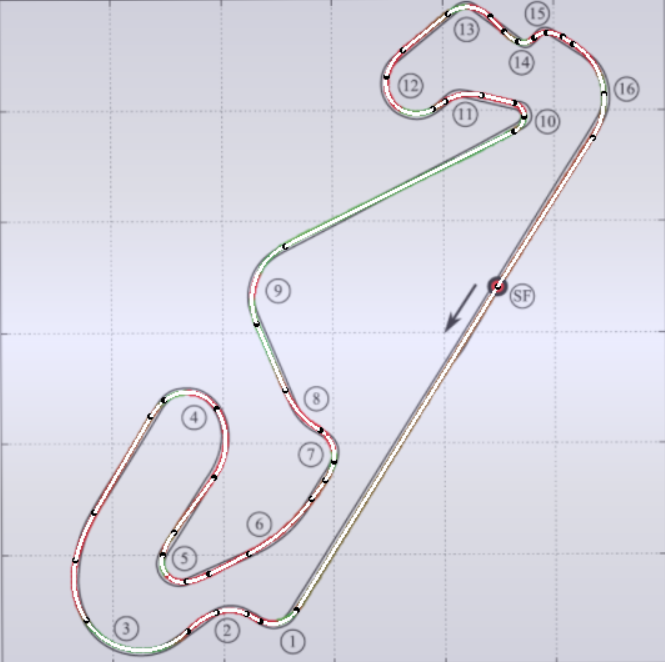
\includegraphics[width=0.6\textwidth]{figures/barcelona_curvilinear2.png}
    \end{center}
    \caption{Αποτύπωση πίστας \textit{Circuit de Barcelona - Catalunya} σε καμπυλόγραμμες συντεταγμένες.}
\label{fig:barcelonaCurvilinear}
\end{figure}

Η διαμήκης επιτάχυνση κατά μήκος της τροχιάς υπολογίζεται με παραγώγιση της σειράς της ταχύτητας $U_{\hat{X}}(s)$ με κεντρικές πεπερασμένες διαφορές. Σημειώνεται πως στην υλοποίηση, το πεδίο της ταχύτητας εξομαλύνθηκε με μέθοδο Savitzky \& Golay \cite{SavitzkyGolay1964}, για την αποφυγή διάδοσης θορύβου λόγω της αριθμητικής παραγώγισης.

\begin{equation}
    a_{\hat{X}}(s_i) = \dfrac{U_{\hat{X}}(s_{i+1}) - U_{\hat{X}}(s_{i-1})}{2h}
    \label{eq:finDiffAx}
\end{equation}

Και η πλευρική επιτάχυνση εκφρασμένη στο κινούμενο σύστημα αξόνων $\hat{X}\hat{Y}$ δίνεται στην \cref{eq:kinematicAy}. Εξ'ορισμού, η συνιστώσα $U_{\hat{Y}} = 0$ καθώς το σύστημα ορίζεται με τον άξονα $\hat{X}$ στη διεύθυνση της ταχύτητας του κέντρου μάζας.

\begin{equation}
    a_{\hat{Y}} = \dfrac{dU_{\hat{Y}}}{dt} = 0
    \label{eq:kinematicAy}
\end{equation}

Σημειώνεται πως η παραπάνω σχέση αφορά τη μεταβολή της συνιστώσας της ταχύτητας στο κινούμενο σύστημα αξόνων· η κεντρομόλος επιτάχυνση $U_{\hat{X}}\dot{\psi}$ λαμβάνεται υπόψη μέσω του όρου $M\dot{\psi}U$ των εξισώσεων κίνησης (\cref{eq:vehicleMotion1,eq:vehicleMotion2}).


Για τον υπολογισμό του ρυθμού εκτροπής θεωρούνται συνθήκες μόνιμης κατάστασης. Στην πράξη, στην είσοδο και έξοδο της στροφής το όχημα βρίσκεται σε μεταβατική κατάσταση, ωστόσο, παραδεχόμαστε πως αυτό το μεταβατικό τμήμα συμβαίνει σε μικρό ποσοστό του γύρου και δεν επηρεάζει σημαντικά τη συνολική εξέλιξη της θερμοκρασίας και της φθοράς. Επομένως, για συνθήκες μόνιμης κατάστασης, ο ρυθμός εκτροπής είναι:

\begin{equation}
    \dot{\psi}(s) = \dfrac{U_{\hat{X}}(s)}{R(s)}
    \label{eq:steadyStateYawRate}
\end{equation}

\subsection{Κατάστρωση εξισώσεων}
\label{subsec:stateSolverEquations}
Για τη διατύπωση του μαθηματικού προβλήματος ξεκινάμε με την καταγραφή των άγνωστων μεγεθών. Για την απλοποίηση της διατύπωσης, ξεκινάμε με τον υπολογισμό των γνωστών μεγεθών.\\
\noindent
Με βάση τις εξισώσεις που αναπτύχθηκαν στα \cref{sec:tyre_model,sec:vehicle_model}, το σύνολο των άγνωστων μεταβλητών δίνεται στον παρακάτω πίνακα.

\begin{table}[htbp]
    \centering
    \small
    \renewcommand{\arraystretch}{1.2}
    \begin{tabular}{@{}l l@{}}
        \toprule
        \textbf{Μεταβλητή} & \textbf{Περιγραφή} \\
        \midrule
        $\boldsymbol{\beta}$         & \textbf{Γωνία πλευρικής ολίσθησης οχήματος} \\
        $\boldsymbol{\delta}$        & \textbf{Γωνία διεύθυνσης εμπρός τροχών} \\
        \midrule
        $F_x$           & Συνολικό διαμήκες φορτίο οχήματος \\
        $F_y$           & Συνολικό πλευρικό φορτίο οχήματος \\
        \midrule
        $F_{x,y,z,FL}$  & Φορτία τροχού FL \\
        $F_{x,y,z,FR}$  & Φορτία τροχού FR \\
        $F_{x,y,z,RL}$  & Φορτία τροχού RL \\
        $F_{x,y,z,RR}$  & Φορτία τροχού RR \\
        \midrule
        $\kappa_{FL}$   & Λόγος ολίσθησης τροχού FL \\
        $\kappa_{FR}$   & Λόγος ολίσθησης τροχού FR \\
        $\kappa_{RL}$   & Λόγος ολίσθησης τροχού RL \\
        $\kappa_{RR}$   & Λόγος ολίσθησης τροχού RR \\
        \midrule
        $\alpha_{FL}$   & Γωνία ολίσθησης τροχού FL \\
        $\alpha_{FR}$   & Γωνία ολίσθησης τροχού FR \\
        $\alpha_{RL}$   & Γωνία ολίσθησης τροχού RL \\
        $\alpha_{RR}$   & Γωνία ολίσθησης τροχού RR \\
        \bottomrule
    \end{tabular}
    \caption{Σύνολο αγνώστων μοντέλου εκτίμησης κατάστασης.}
    \label{tab:stateUnknowns}
\end{table}

Από την κατάστρωση των αγνώστων προκύπτει πως το μοντέλο έχει 24 άγνωστα μεγέθη. Το σύστημα των 24 εξισώσεων δε διαθέτει λύση κλειστού τύπου επομένως θα επιλυθεί αριθμητικά.
Ωστόσο, η αριθμητική διαδικασία μπορεί να επιταχυνθεί αν πραγματοποιήσουμε μια προ-επεξεργασία, συσχετίζοντας αναλυτικά τις άγνωστες ποσότητες μεταξύ τους. Πράγματι, όπως θα αναπτυχθεί παρακάτω, όλα τα άγνωστα μεγέθη μπορούν να εκφρασθούν μονοσήμαντα συναρτήσει των γωνιών $\beta$ και $\delta$, μειώνοντας το πρόβλημα σε ένα σύστημα μη-γραμμικών εξισώσεων $2\times2$. Η διαδικασία των αντικαταστάσεων στις εξισώσεις καλύπτεται εν μέρει από το σχεδιάγραμμα της επίλυσης \ref{fig:slip_est_flow}. \\[6pt]

\subsubsection{Υπολογισμός ταχυτήτων και επιταχύνσεων}

\noindent
Αρχικά, υπολογίζονται οι επιταχύνσεις στο τοπικό σύστημα του οχήματος $\alpha_x, \alpha_y$ με μετασχηματισμό \ref{eq:vectorTransformations}.

\begin{equation}
    \begin{aligned}
         \begin{Bmatrix}
            \alpha_x \\ \alpha_y
        \end{Bmatrix}
        &= R(\beta)
        \begin{Bmatrix}
            \alpha_{\hat{X}} \\ \alpha_{\hat{Y}}
        \end{Bmatrix}\\[10pt]
         \begin{Bmatrix}
            U_x \\ U_y
        \end{Bmatrix}
        &= R(\beta)
        \begin{Bmatrix}
            U_{\hat{X}} \\ U_{\hat{Y}}
        \end{Bmatrix}
    \end{aligned}
    \label{eq:localAccelAndVelocity}
\end{equation}

\noindent
Έπειτα, υπολογίζονται οι συνιστώσες της ταχύτητας κάθε τροχού, μέσω της εξίσωσης (\ref{eq:wheelVelocity}).\\[5pt]

\noindent
Για τους εμπρόσθιους τροχούς, τα διανύσματα των ταχυτήτων μετασχηματίζονται στο τοπικό σύστημα των τροχών ως:

\begin{equation}
    \vec{U}_{uv,i} = R(-\delta)\vec{U}_{xy,i}
    \label{eq:wheelVelocityTransformation}
\end{equation}

 \noindent
 Επομένως, από την \cref{eq:slipAngleCalculation} υπολογίζονται οι γωνίες ολίσθησης κάθε τροχού.

\begin{equation}
    \alpha_i = tan^{-1}\Bigl(\dfrac{U_{v,i}}{U_{u,i}}\Bigr)
    \label{eq:slipAngleCalculation}
\end{equation}

\subsubsection{Υπολογισμός δυνάμεων}
\noindent
Έχοντας υπολογίσει τις επιταχύνσεις και τις ταχύτητες του οχήματος στο τοπικό του σύστημα αξόνων, υπολογίζονται τα συνολικά φορτία του αμαξώματος $F_x, F_y$, μέσω των εξισώσεων (\ref{eq:vehicleMotion1}) και (\ref{eq:vehicleMotion2}).

\noindent
Παράλληλα, υπολογίζονται μέσω των εξισώσεων (\ref{eq:drag})--(\ref{eq:liftRear}) η οπισθέλκουσα $F_{x,drag}$ και η αρνητική άνωση (downforce) στους δύο άξονες $F_{z,f,lift}, F_{z,r,lift}$.\\[5pt]

Και τα κατακόρυφα φορτία των τροχών $F_{z,i}$ υπολογίζονται από τις σχέσεις (\ref{eq:longitudinalWeightTransfer}), (\ref{eq:lateralWeightTransfer}) και (\ref{eq:normalLoads}). Τα τελικά κατακόρυφα φορτία διορθώνονται σε περίπτωση απώλειας επαφής, για αποφυγή λανθασμένων αποτελεσμάτων.

\begin{equation}
    \begin{aligned}
        F_{z,i,\text{διορθ.}} &= max(F_{z,i}, 0)\\
        F_{z,i,\text{παραβ.}} &= min(F_{z,i}, 0)
    \end{aligned}
    \label{eq:fzViolation}
\end{equation}

\noindent
Όπου $F_{z,i,\text{παραβ.}}$, είναι το ποσό του φορτίου που παραβιάζει τη συνθήκη επαφής.\\[2.5pt]

\noindent
Ένα αποτέλεσμα αυτής της προσέγγισης είναι πως όταν ένας τροχός χάσει επαφή με το έδαφος, δεν επανα-κατανέμεται το κατακόρυφο φορτίο στους υπόλοιπους τρεις τροχούς, επομένως δεν ισχύει πλέον ισορροπία δυνάμεων στον κατακόρυφο άξονα, ωστόσο, αυτό αναμένεται να μην εισάγει παρατηρήσιμο σφάλμα στα αποτελέσματα.\\[5pt]

Έχοντας υπολογίσει τις γωνίες ολίσθησης και τα κατακόρυφα φορτία, πλέον τα εγκάρσια φορτία υπολογίζονται από το μοντέλο ελαστικών της μορφής της (\ref{eq:tyreModelFinal}). Το μοντέλο ελαστικών λαμβάνει ως είσοδο το απαιτούμενο διαμήκες φορτίο, το οποίο κατά περίπτωση θα αναλυθεί στην επόμενη παράγραφο.\\[5pt]

\noindent
Τα φορτία των ελαστικών μετασχηματίζονται τελικά στο σύστημα του οχήματος:

\begin{equation}
    \vec{F}_{xy,i} = R(\delta)\vec{F}_{uv,i}
    \label{eq:tyreForcesTransformation}
\end{equation}

\subsubsection{Υπολογισμός διαμήκων φορτίων}
\noindent
Η συνισταμένη διαμήκης δύναμη του οχήματος δίνεται παρακάτω.

\begin{equation}
    F_x = F_{x,tires} + F_{x,drag}
    \label{eq:vehicleFx}    
\end{equation}

\noindent
Όπου $F_{x,tires}$ η συνισταμένη διαμήκης δύναμη που παράγουν τα ελαστικά, εκφρασμένη στο σύστημα αξόνων του οχήματος. Αντικαθιστώντας την (\ref{eq:vehicleFx}) στην \cref{eq:vehicleMotion1}, προκύπτει:

\begin{equation}
    F_{x,tires} = M\dfrac{d}{dt}U_x(t) - M\dot{\psi} U_y - F_{x,drag}
    \label{eq:modifiedVehicleMotionX}
\end{equation}

\noindent
Όπου $F_{x,tires}$
\begin{equation}
   F_{x,tires} = F_{x,FL} +  F_{x,FR} +F_{x,RL} +F_{x,RR}
   \label{eq:tyreTotalFx}
\end{equation}

\noindent
Όπου οι δύο πρώτοι όροι του δεξιού μέλους είναι ήδη γνωστοί από τις εξισώσεις (\ref{eq:localAccelAndVelocity}). Καθώς η τιμή του $F_{x,drag}$ είναι εξ'ορισμού αρνητική, η \cref{eq:modifiedVehicleMotionX} μας δείχνει πως όταν το όχημα επιβραδύνει, η οπισθέλκουσα μειώνει το απαιτούμενο φορτίο πέδησης που πρέπει να παρέχουν τα ελαστικά. Αντίθετα, όταν το όχημα επιταχύνει, τα ελαστικά πρέπει, εκτός από τα αδρανειακά, να παρέχουν επιπλέον φορτίο για να υπερνικήσουν την οπισθέλκουσα.\\[6pt]

\noindent
Επομένως, πλέον είναι καθορισμένο το συνολικό διαμήκες φορτίο που πρέπει να παράξουν οι τροχοί. Για τον καθορισμό της κατανομής του φορτίου στους τροχούς ($F_{x,i}, i\in \{FL, FR, RL, RR\}$), διακρίνουμε δύο περιπτώσεις, την πρόωση και την πέδηση. 
Αναπτύσσοντας το συνολικό φορτίο που παράγουν οι τροχοί, οι κινητήριοι τροχοί (πίσω τροχοί) λαμβάνουν το παρακάτω φορτίο.

\begin{equation}
    F_{x,rear} = F_{x,RL} + F_{x,RR} = F_{x,tires} - F_{x,FL} - F_{x,FR}
    \label{eq:rearTractiveForce}
\end{equation}

\begin{figure}[htbp]
    \centering
    % figures/fig_steering_and_forces.tex
% Wheel steered by angle delta with forces F_x, F_y in the local frame
\begin{tikzpicture}[>=Latex, thick, font=\small]

    \def\deltaFig{25}          % steering angle in degrees

    % ---- Wheel rectangle (top view), rotated by delta about the origin ----
    \begin{scope}[rotate=\deltaFig]
    \draw[thick, fill=black!5, rounded corners=8pt] (-1.5, -2.5) rectangle (1.5, 2.5);
    \end{scope}

    % ---- Vehicle reference frame axes ----
    \draw[dashed,->, thick] (0,0) -- (0,5) node[right] {$x$};
    \draw[dashed,->, thick] (0,0) -- (-4,0) node[below]  {$y$};

 % ---- Wheel direction (rotated by delta from vehicle x) ----
    \draw[dashed, gray!100, ->] (0,0) -- ({5*sin(-\deltaFig)}, {5*cos(-\deltaFig)}) node[right] {$u$};

    \draw[dashed, gray!100, ->] (0,0) -- ({-5*cos(-\deltaFig)}, {5*sin(-\deltaFig)}) node[below] {$v$};

    % ---- Reference dashed line (vehicle x direction, along wheel center) ----
    \draw[dashed, gray!60] (0,-2) -- (0,0);

    % ---- Steering angle arc ----
    \draw[<->] (0,4) arc[start angle=90, end angle={90+\deltaFig}, radius=4]
        node[midway, above, yshift=1pt] {$\delta$};

    % ---- Wheel-center coordinate (used to anchor force vectors) ----
    \coordinate (W) at ({0}, {0});
    \fill (W) circle (1pt);

    % ---- Forces in the WHEEL local frame ----
    % F_x along wheel longitudinal axis (rolling direction)
    % F_y perpendicular to wheel plane (lateral)
    \draw[->, thick] (W) -- ++({-3*cos(-\deltaFig)}, {3*sin(-\deltaFig)})
        node[above left]  {$F_v$};

    \draw[->, thick] (0,0) -- (0,{3*sin(-\deltaFig)}) node[right] {$F_x$};
    \draw[dashed, gray!60] (0,{3*sin(-\deltaFig)}) -- ({-3*cos(-\deltaFig)},{3*sin(-\deltaFig)});
    \draw[->, thick] (0,0) -- ({-3*cos(-\deltaFig)},0) node[above] {$F_y$};
    \draw[dashed, gray!60] ({-3*cos(-\deltaFig)},0) -- ({-3*cos(-\deltaFig)},{3*sin(-\deltaFig)});

\end{tikzpicture}
    \caption{Ανάλυση δυνάμεων κατευθυντήριου τροχού -- επαγόμενη αντίσταση}
    \label{fig:inducedDrag}
\end{figure}

Στο \cref{fig:inducedDrag} παρατηρείται πως ένας κατευθυντήριος τροχός, ακόμη και αν δεν παράγει διαμήκη δύναμη στο τοπικό του σύστημα, εισάγει διαμήκες φορτίο στο σύστημα αξόνων του οχήματος. Αυτός είναι ένας από τους λόγους που όταν ένα όχημα στρίβει, δε διατηρεί την ταχύτητά του αλλά επιβραδύνει.

Επομένως, οι περιπτώσεις πρόωσης και πέδησης διακρίνονται παρακάτω. Ολόκληρη η διαδικασία υπολογισμού των διαμήκων φορτίων συνοψίζεται στο \cref{fig:force_distribution_flow}.

\[
    \begin{cases}
        \text{Πρόωση}   & \text{αν } F_{x,rear} \geq 0 \\
        \text{Πέδηση}   & \text{αν } F_{x,rear} < 0 
    \end{cases}
\]


\paragraph{Περίπτωση πρόωσης}
Στην περίπτωση που το όχημα βρίσκεται σε κατάσταση πρόωσης, οι κινητήριοι τροχοί (πίσω) παρέχουν ολόκληρο το ποσό του φορτίου πρόωσης, ενώ για τους εμπρόσθιους τροχούς ισχύει $F_{u,FL},F_{u,FR} = 0$. Η διανομή του συνολικού φορτίου πρόωσης στους δύο τροχούς του άξονα πραγματοποιείται μέσω του διαφορικού, και μοντελοποιείται μέσω της σχέσης (\ref{eq:differential}), αντικαθιστώντας την \cref{eq:rearTractiveForce}.

\paragraph{Περίπτωση πέδησης}
Στην κατάσταση πέδησης, τα φορτία διανέμονται στον εμπρός και πίσω άξονα μέσω της σχέσης (\ref{eq:brakingDistribution}). Τα φορτία του κάθε άξονα θεωρούνται πως ισο-μοιράζονται στους δύο τροχούς.

\paragraph{Κορεσμός}
Σε δυναμικές συνθήκες, το ελαστικό μπορεί να μην έχει τη δυνατότητα να παράξει το απαιτούμενο φορτίο στις συνθήκες που βρίσκεται. Σε αυτή την περίπτωση, το διάνυσμα της λύσης του συστήματος κρίνεται ανέφικτο, αποδίδεται στο μοντέλο το μέγιστο φορτίο που είναι διαθέσιμο από το ελαστικό και καταγράφεται το έλλειμμα για τους σκοπούς των περιορισμών που αναλύεται σε επόμενη παράγραφο. 

\begin{equation}
    F_{x,i,\text{έλλειμμα}} = max\Bigl(
    \bigl(F_{x,i,\text{ζητ.}} - F_{x,i,\text{διαθ.}}\bigr), 0\Bigr)
    \label{eq:fxViolation}
\end{equation}

\begin{figure}[htbp!]
\centering
\begin{tikzpicture}[
    node distance=0.6cm and 1.0cm,
    block/.style   ={rectangle, draw=black, fill=white,   text width=8cm,
                     align=center, rounded corners=4pt, minimum height=0.9cm, font=\small},
    io/.style      ={rectangle, draw=black, fill=black!5, text width=6cm,
                     align=center, rounded corners=2pt, minimum height=0.9cm, font=\small},
    outbox/.style  ={rectangle, draw=black, fill=black!12, text width=6cm,
                     align=center, rounded corners=2pt, minimum height=0.9cm, font=\small\bfseries},
    decision/.style={diamond,   draw=black, fill=white,   text width=2.6cm,
                     align=center, font=\scriptsize, inner sep=1pt},
    arr/.style     ={->, thick, black}
]

  \node[block]          (fyFront)  {Υπολογισμός πλευρικής δύναμης εμπρόσθιων τροχών $F_{y,front,0}$\\ υπό υπόθεση $F_x = 0$};
  \node[block, below=of fyFront]                  (fxRear)   {Εκτίμηση απαιτούμενης διαμήκους δύναμης οπίσθιων τροχών ($F_{x,rear,0}$)};
  \node[decision, below=of fxRear]                (sign)     {$F_{x,rear,0} \geq 0$;};

  % --- Traction branch (right) ---
  \node[block, right=1.6cm of sign, xshift=1.2cm] (traction) {Πρόωση:\\ κατανομή $F_{x,rear,0}$  στους δύο\\ κινητήριους τροχούς};

  % --- Braking branch (left) ---
  \node[block, below=1.4cm of sign]               (splitBrk) {Πέδηση:\\ διανομή συνολικής δύναμης\\ πέδησης εμπρός/πίσω $F_{x,front}, F_{x,rear}$};
  \node[block, below=of splitBrk]                 (recFy)    {Επανυπολογισμός $F_{y,front}$ λαμβάνοντας υπόψη νέα $F_{x,front}$};
  \node[block, below=of recFy]                    (recFxr)   {Επανυπολογισμός $F_{x,rear}$ και κατανομή στους κινητήριους τροχούς};

  % --- Output ---
  \node[outbox, below=1.4cm of recFxr]            (out)      {Έξοδος: δυνάμεις $F_x, F_y$ ανά τροχό};

  % --- Arrows ---
  \draw[arr] (fyFront) -- (fxRear);
  \draw[arr] (fxRear)  -- (sign);

  % Braking branch (straight down)
  \draw[arr] (sign)    -- node[right]{όχι (πέδηση)} (splitBrk);
  \draw[arr] (splitBrk) -- (recFy);
  \draw[arr] (recFy)   -- (recFxr);
  \draw[arr] (recFxr)  -- (out);

  % Traction branch (right, then down and back)
  \draw[arr] (sign.east) -- node[above]{ναι (πρόωση)} (traction.west);
  \draw[arr] (traction.south) |- (out.east);

\end{tikzpicture}
\caption{Διάγραμμα ροής -- διαδικασία υπολογισμού διαμήκων φορτίων πρόωσης και πέδησης.}
\label{fig:force_distribution_flow}
\end{figure}

\subsubsection{Τελικό σύστημα εξισώσεων}

Μετά από όλους του υπολογισμούς του κεφαλαίου, το σύστημα εξισώσεων προς επίλυση διαμορφώνεται από τις δύο εξισώσεις κίνησης (\ref{eq:vehicleMotion2}) και (\ref{eq:vehicleMotion3}) σε μόνιμη κατάσταση $\Bigl(\dfrac{d}{dt}\dot{\psi}(t)\Bigr)$.

\begin{equation}
    \left\{
    \begin{aligned}
        M\dfrac{d}{dt}U_y(t) + M\dot{\psi}U_x - \sum_{i=FL,\dots,RR}\Bigl(F_{y,i}\Bigr) &= 0 \\[5pt]
        \sum_{i=FL,\dots,RR} \Bigl(\vec{r}_i\times\vec{F}_i\Bigr)_z &= 0
    \end{aligned}
    \right.
    \label{eq:stateSolverEquationSystem}
\end{equation}

\subsection{Αριθμητικός επιλύτης}
\label{subsec:stateSolverNumerical}
Η επίλυση του συστήματος γίνεται με αριθμητική μέθοδο όπως έχει ήδη αναφερθεί. Καθώς τα δεδομένα μπορεί να βασιστούν σε προσεγγίσεις, ενώ επίσης ολόκληρη η διαδικασία αποτελεί μια εκτίμηση, είναι φυσικό σε κάποια σημεία λειτουργίας, το μοντέλο να μη βρει δυνατές λύσεις εντός των περιορισμών. Για τον λόγο αυτό, επιλέχθηκε η χρήση αλγορίθμου ελαχιστοποίησης ($min(f)$), έναντι επίλυσης ισότητας (λ.χ. \textit{Newton-Raphson}), ώστε σε αδύνατα σημεία του επιλύτη, να λάβουμε την κοντινότερη φυσική λύση που μπορεί να παράξει τη ζητούμενη κατάσταση.\\[10pt]

\noindent
Οι ελεύθερες μεταβλητές $\beta,\ \delta$ περιορίζονται ώστε να αποφευχθούν μη-φυσικές λύσεις.

\begin{equation*}
    \begin{aligned}
        \beta\ &\in\ [-15^\circ,15^\circ]\\
        \delta\ &\in\ [-45^\circ,45^\circ]       
    \end{aligned}
\end{equation*}

\subsubsection{Ορισμός αντικειμενικής συνάρτησης}

Ως αντικειμενική συνάρτηση επιλέγεται το τετράγωνο των υπολοίπων του συστήματος εξισώσεων (\ref{eq:stateSolverEquationSystem}).

\begin{equation}
    \left\{
    \begin{aligned}
        f_1(\mathbf{x}) &= \Biggl(M\dfrac{d}{dt}U_y(t) + M\dot{\psi}U_x - \sum_{i=FL,\dots,RR}\Bigl(F_{y,i}\Bigr)\Biggr)^2 \\[5pt]
        f_2(\mathbf{x}) &= \Biggl(\sum_{i=FL,\dots,RR} \Bigl(\vec{r}_i\times\vec{F}_i\Bigr)_z \Biggr)^2
    \end{aligned}
    \right.
    \label{eq:stateSolverResiduals}
\end{equation}

Επομένως, το πρόβλημα εμπίπτει στην ελαχιστοποίηση των αντικειμενικών συναρτήσεων $f_1(\mathbf{x}),f_2(\mathbf{x})$. Η επίλυση γίνεται μέσω της συνάρτησης \textit{lsqnonlin} της \textit{Matlab} \cite{mathworks_lsqnonlin}.

\subsubsection{Υλοποίηση περιορισμών}

Στους αλγορίθμους βελτιστοποίησης, η μέθοδος εφαρμογής των περιορισμών αποτελεί βασικότατο παράγοντα που επηρεάζει την ταχύτητα αλλά και την ικανότητα εύρεσης του βέλτιστου. Οι περιορισμοί δεν παίζουν απλά τον ρόλο της σήμανσης μιας λύσης ως ανέφικτη, αλλά βοηθούν τον αλγόριθμο να επιλέξει εφικτή λύση "στρίβοντάς" τον προς τον εφικτό χώρο. Συνήθως αυτό επιτυγχάνεται με την επιβολή ποινής στην αντικειμενική συνάρτηση και χρησιμοποιούνται διάφορες προσεγγίσεις κλιμακοποίησης των ποινών \cite{nocedal2006numerical}. Στην υλοποίηση της παρούσας εργασίας, υπολογίζεται η τιμή της παραβίασης των περιορισμών και ο επιλύτης \textit{lsqnonlin} διαχειρίζεται την εφαρμογή των ποινών.
\noindent
\paragraph{Διαθέσιμη πρόσφυση ελαστικών}
Ο πρώτος περιορισμός είναι η δυνατότητα των ελαστικών να παρέχουν τα ζητούμενα φορτία. Όπως αναλύθηκε παραπάνω (\cref{eq:fxViolation}), η συνάρτηση του περιορισμού ορίζεται ως

\begin{equation}
    g_1(\mathbf{x}) = \sum_{i=FL,\dots,RR}\Bigl(F_{x,i,\text{έλλειμμα}}\Bigr)
\label{eq:totalFxViolation}
\end{equation}


\paragraph{Συνθήκη μη-ανατροπής}
Για την αποφυγή ανατροπής, ελέγχεται η ταυτόχρονη απώλεια κάθετου φορτίου σε
ζεύγη τροχών που ορίζουν πιθανό άξονα περιστροφής του οχήματος. Ορίζουμε το
σύνολο των κρίσιμων ζευγών
\begin{equation}
    \mathcal{P} = \bigl\{(FL,RL),\ (FR,RR),\ (FL,FR),\ (RL,RR)\bigr\},
\end{equation}
που αντιστοιχούν στην αριστερή και δεξιά πλευρά, καθώς και στον εμπρός και
πίσω άξονα. Για κάθε ζεύγος $(i,j)\in\mathcal{P}$, η συνεισφορά στη
συνάρτηση παραβίασης δίνεται ως

\begin{equation}
    \Pi_{(i,j)} =
    \begin{dcases}
        F_{z,i,\text{παραβ.}} + F_{z,j,\text{παραβ.}} & ,F_{z,i} < 0 \ \text{και}\ F_{z,j} < 0 \\
        0 & ,\text{σε κάθε άλλη περίπτωση}
    \end{dcases}
\end{equation}

και η συνολική συνεισφορά της συνθήκης μη-ανατροπής προκύπτει από την
άθροιση επί όλων των ζευγών,
\begin{equation}
    g_2(\mathbf{x}) = \sum_{(i,j)\in\mathcal{P}}\Pi_{(i,j)}
    \label{eq:noRolloverConstraint}
\end{equation}
Η διατύπωση αυτή επιτρέπει τη μεμονωμένη ανύψωση ενός τροχού --
αναμενόμενη κατάσταση σε έντονη εγκάρσια ή διαμήκη μεταφορά φορτίου -- χωρίς
να επιβάλλεται ποινή.

\subsection{Εξαγωγή αποτελεσμάτων}

\subsubsection{Μεταβλητές κατάστασης}

Το αποτέλεσμα της αριθμητικής επίλυσης είναι το ζεύγος γωνιών $\beta,\ \delta$ που ικανοποιούν τις εξισώσεις ισορροπίας σε μόνιμη κατάσταση. Χρησιμοποιώντας τη μεθοδολογία της ενότητας \ref{subsec:stateSolverEquations}, υπολογίζονται όλες οι μεταβλητές κατάστασης του πίνακα \ref{tab:stateUnknowns}.\\[10pt]

Παρακάτω παρατίθενται ενδεικτικά αποτελέσματα από επίλυση στην πίστα της Βαρκελώνης \textit{Circuit de Barcelona - Catalunya}. Σημειώνεται πως στο \cref{fig:carInCorner} οι γωνίες $\beta,\ \delta$ είναι αυξημένες για οπτικούς λόγους -- οι πραγματικές γωνίες δε θα ήταν ευδιάκριτες.

\begin{figure}[htbp!]
    \centering
    \begin{subfigure}[t]{0.32\textwidth}
        \centering
        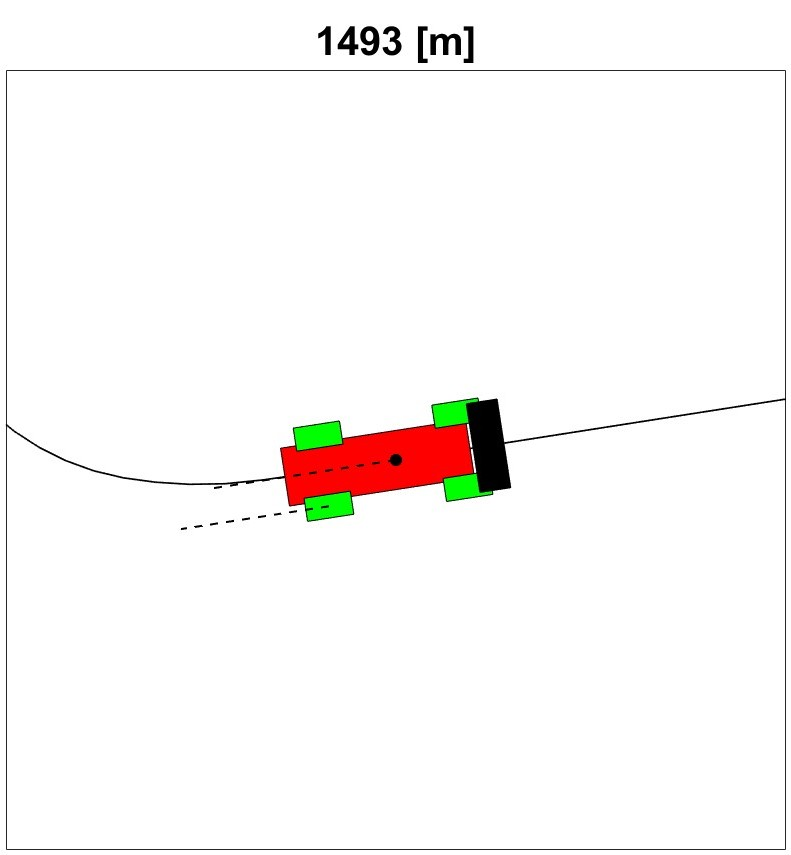
\includegraphics[height=5.5cm]{figures/curveEntry.jpg}
        \caption{Είσοδος στροφής}
        \label{fig:cornerEntry}
    \end{subfigure}
    \hfill
    \begin{subfigure}[t]{0.32\textwidth}
        \centering
        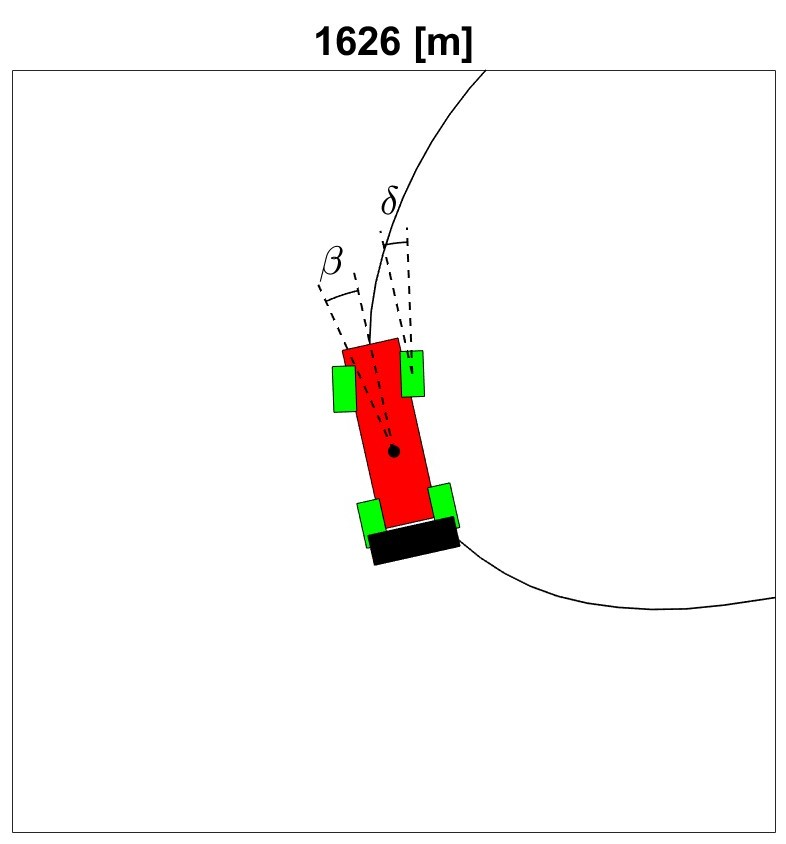
\includegraphics[height=5.5cm]{figures/curveMiddle.jpg}
        \caption{Μέσο στροφής}
        \label{fig:midCorner}
    \end{subfigure}
    \hfill
    \begin{subfigure}[t]{0.32\textwidth}
        \centering
        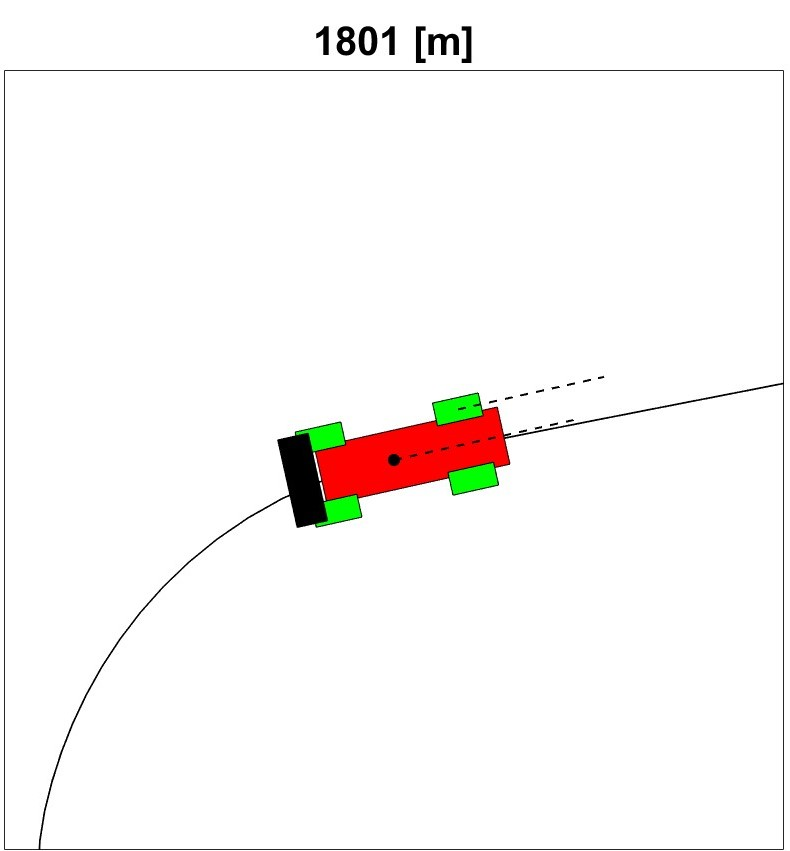
\includegraphics[height=5.5cm]{figures/curveExit.jpg}
        \caption{Έξοδος στροφής}
        \label{fig:cornerExit}
    \end{subfigure}
    \caption{Ενδεικτική σχηματική αναπαράσταση αποτελεσμάτων επίλυσης της κατάστασης οχήματος.}
    \label{fig:carInCorner}
\end{figure}


\begin{figure}[htbp!]
    \centering
    \begin{subfigure}[t]{0.48\textwidth}
        \centering
        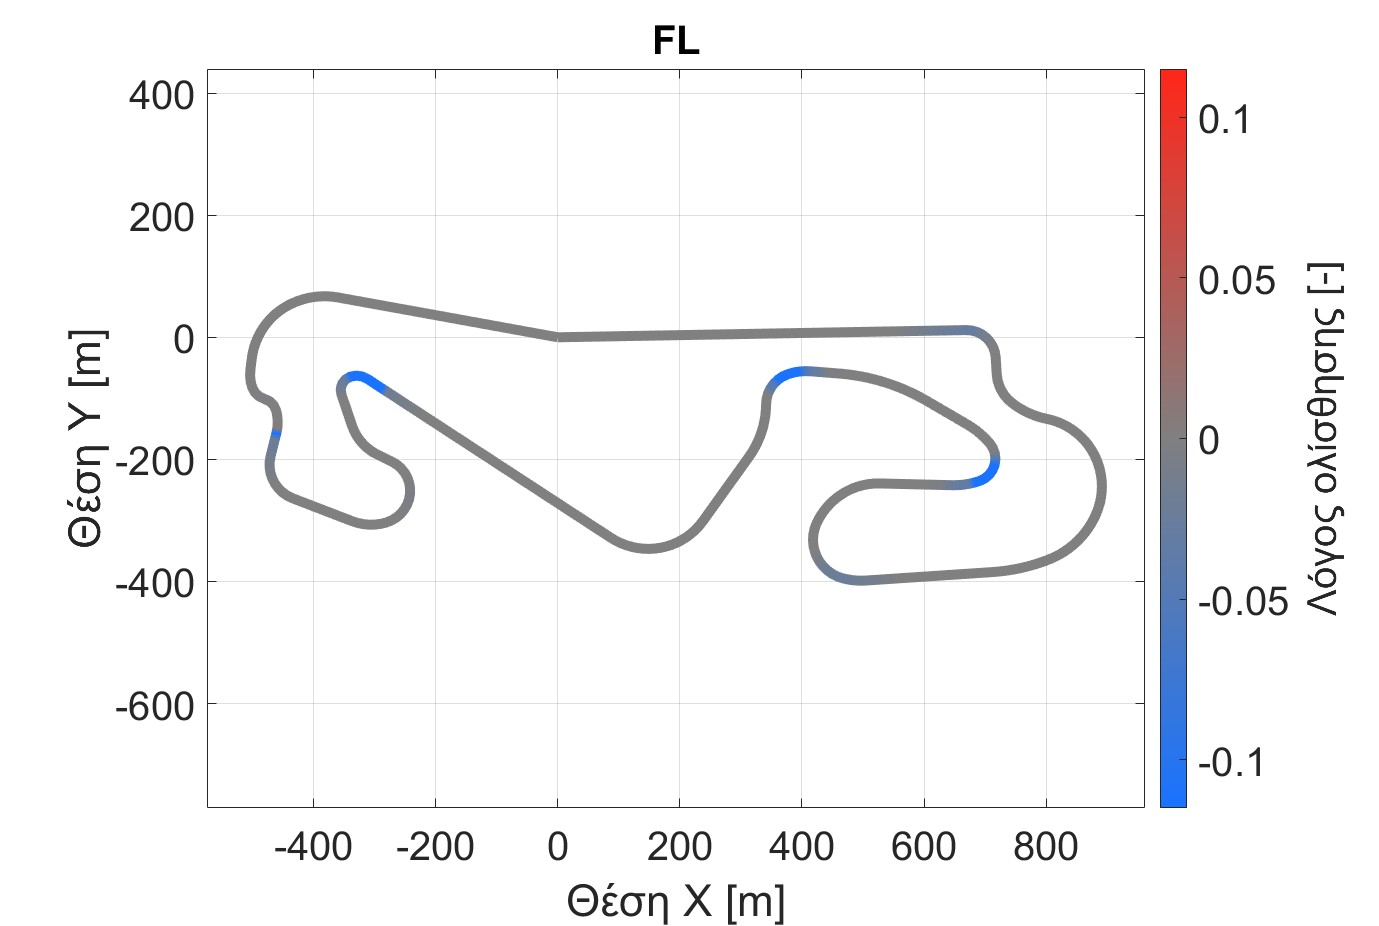
\includegraphics[width=\textwidth]{figures/slipRatioFL.jpg}
    \end{subfigure}
    \hfill
    \begin{subfigure}[t]{0.48\textwidth}
        \centering
        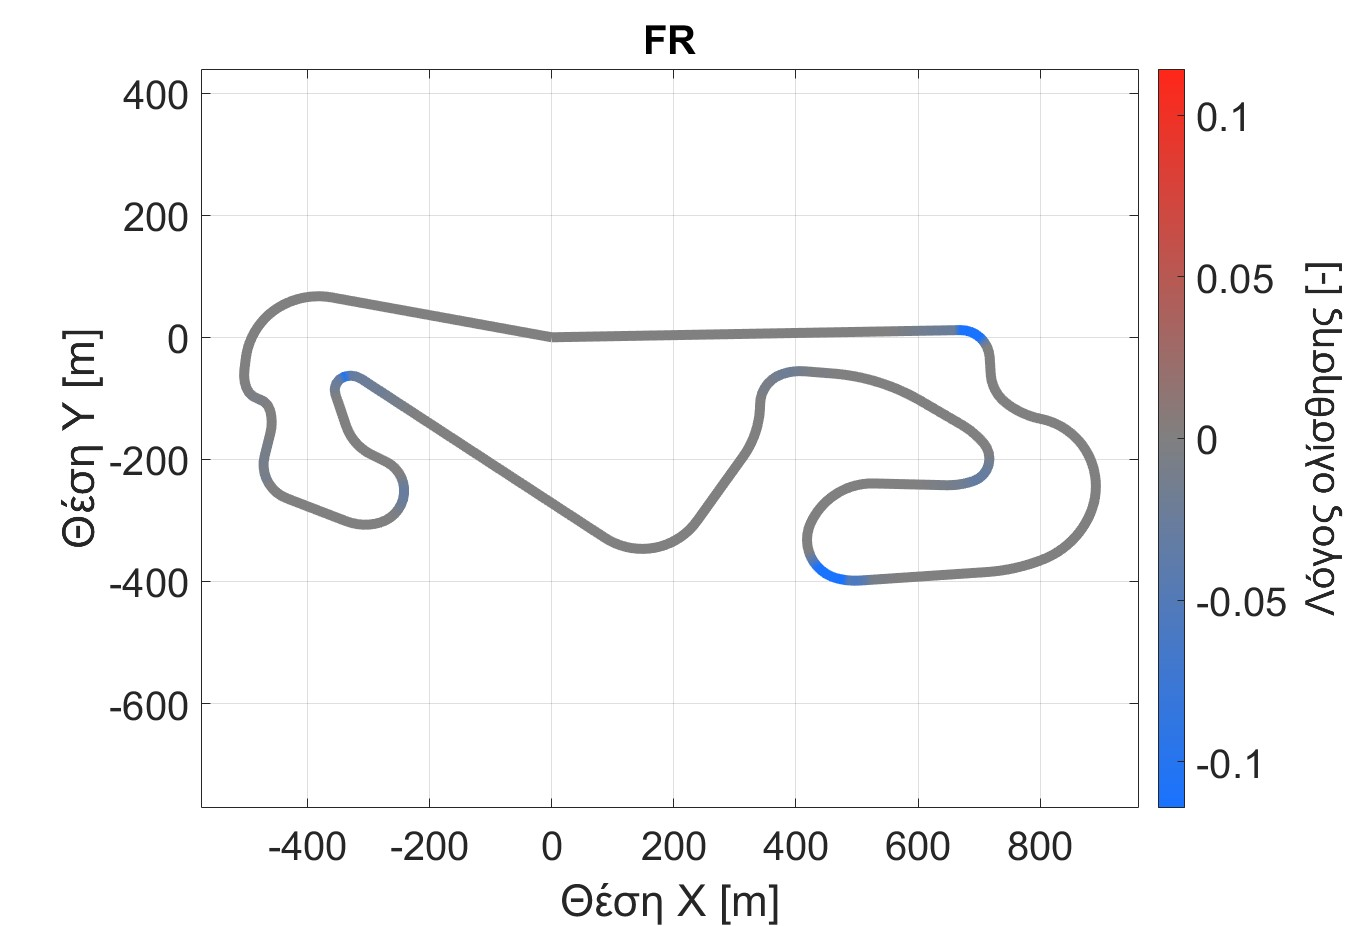
\includegraphics[width=\textwidth]{figures/slipRatioFR.jpg}
    \end{subfigure}

    \vspace{0.5em}

    \begin{subfigure}[t]{0.48\textwidth}
        \centering
        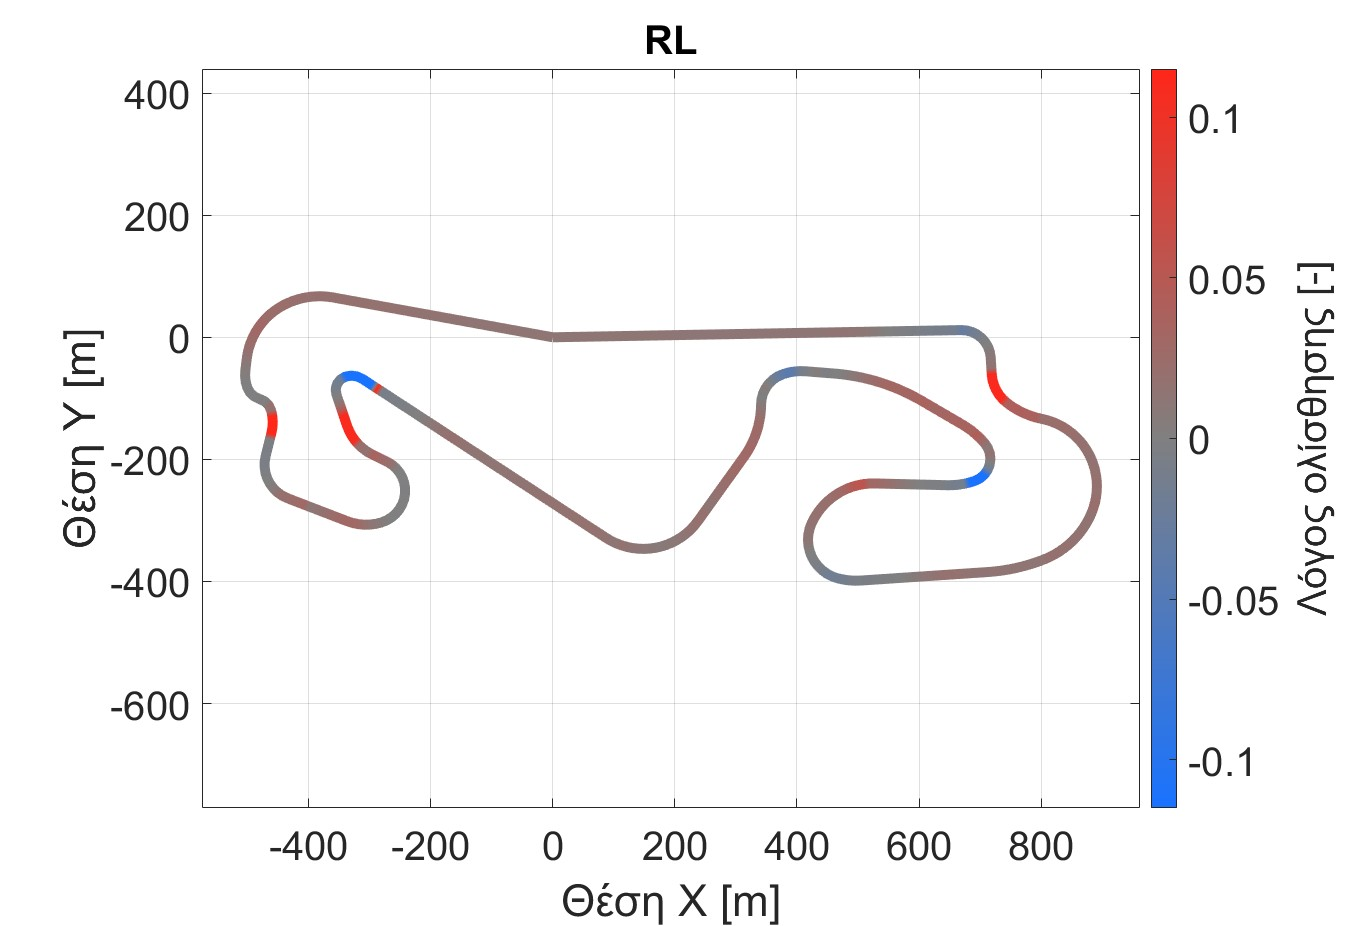
\includegraphics[width=\textwidth]{figures/slipRatioRL.jpg}
    \end{subfigure}
    \hfill
    \begin{subfigure}[t]{0.48\textwidth}
        \centering
        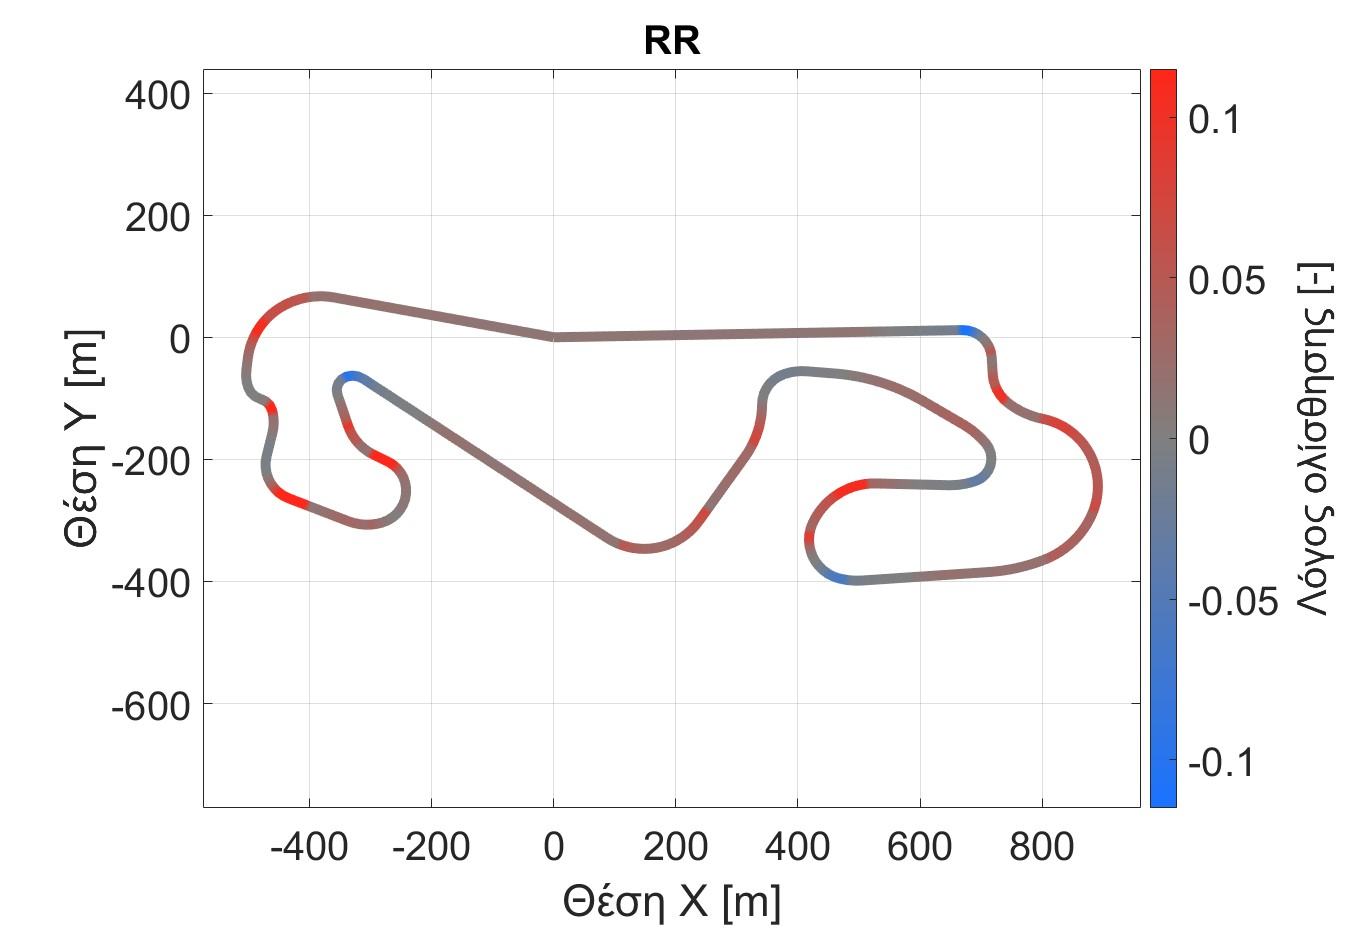
\includegraphics[width=\textwidth]{figures/slipRatioRR.jpg}
    \end{subfigure}
    \caption{Ενδεικτικά αποτελέσματα λόγου ολίσθησης σε γύρο της πίστας \textit{Circuit de Barcelona - Catalunya}}
    \label{fig:slipRatioSamples}
\end{figure}

\begin{figure}[htbp!]
    \centering
    \begin{subfigure}[t]{0.48\textwidth}
        \centering
        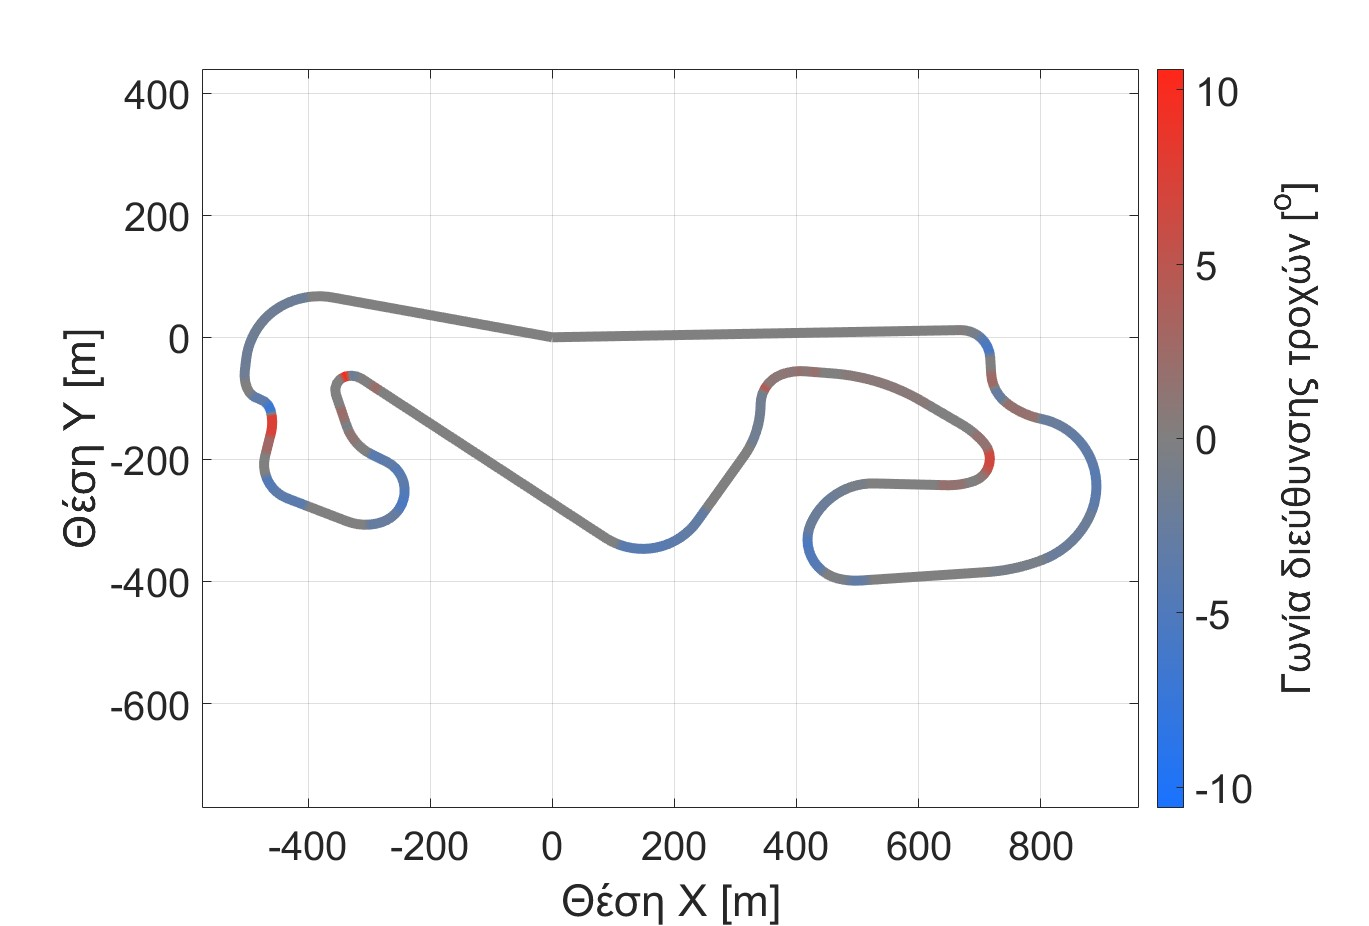
\includegraphics[width=\textwidth]{figures/steerAngle.jpg}
        \caption{Γωνία διεύθυνσης κατευθυντήριων τροχών}
        \label{fig:steerAnglePlot}
    \end{subfigure}
    \hfill
    \begin{subfigure}[t]{0.48\textwidth}
        \centering
        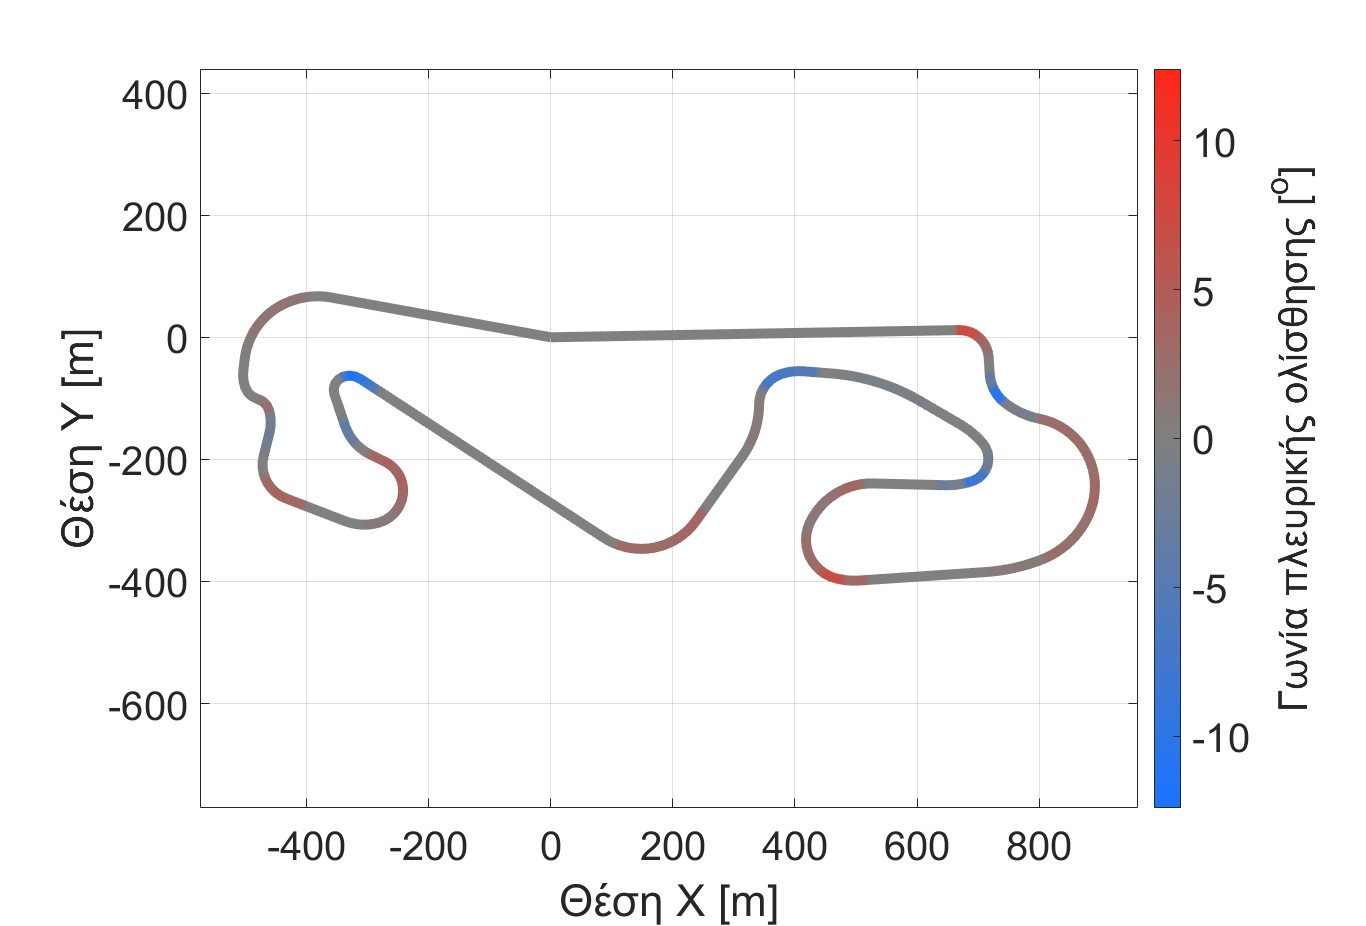
\includegraphics[width=\textwidth]{figures/chassisSlipAngle.jpg}
        \caption{Γωνία πλευρικής ολίσθησης}
        \label{fig:chassisSlipAnglePlot}
    \end{subfigure}
    \caption{Ενδεικτικά αποτελέσματα των μεταβλητών κατάστασης σε γύρο της πίστας \textit{Circuit de Barcelona - Catalunya}}
    \label{fig:solverAngles}
\end{figure}

\subsubsection{Θερμοκρασία και φθορά}

Σε αντίθεση με τις μεταβλητές κατάστασης του πίνακα \ref{tab:stateUnknowns}, η θερμοκρασία και η φθορά δε δίνονται μονοσήμαντα από τη δυναμική κατάσταση του οχήματος, αλλά περιλαμβάνουν την "ιστορία" του οχήματος καθώς αποτελούν ολοκληρώματα των αντίστοιχων ισχύων και ρυθμών φθοράς. Οι \cref{eq:dTds_full,eq:Wtotal} ολοκληρώνονται σε κάθε βήμα διακριτοποίησης της πίστας. Η ολοκλήρωση λαμβάνει χώρα σε κάθε σημείο της πίστας ταυτόχρονα με την επίλυση μόνιμης κατάστασης, καθώς η ανανεωμένη θερμοκρασία και φθορά επηρεάζουν τις καμπύλες πρόσφυσης των ελαστικών, και επομένως, επηρεάζουν την κατάσταση του οχήματος.

\paragraph{Θερμοκρασία}
Για την \cref{eq:dTds_full}, η οποία είναι διατυπωμένη ως προς την απόσταση $s$, εφαρμόζεται το κλασικό σχήμα \textit{Runge-Kutta} 4$^{\text{ης}}$ τάξης. Σε κάθε βήμα $s_n \rightarrow s_{n+1} = s_n + h$:

\begin{equation}
    \begin{aligned}
        k_1 &= \frac{1}{U_{x,n}}\,\dot{T}\!\left(\mathbf{x}_n,\ T_n\right)\\[2pt]
        k_2 &= \frac{1}{U_{x,n+\frac{1}{2}}}\,\dot{T}\!\left(\mathbf{x}_{n+\frac{1}{2}},\ T_n + \tfrac{h}{2}k_1\right)\\[2pt]
        k_3 &= \frac{1}{U_{x,n+\frac{1}{2}}}\,\dot{T}\!\left(\mathbf{x}_{n+\frac{1}{2}},\ T_n + \tfrac{h}{2}k_2\right)\\[2pt]
        k_4 &= \frac{1}{U_{x,n+1}}\,\dot{T}\!\left(\mathbf{x}_{n+1},\ T_n + h\,k_3\right)\\[2pt]
        T_{n+1} &= T_n + \frac{h}{6}\bigl(k_1 + 2k_2 + 2k_3 + k_4\bigr)
    \end{aligned}
    \label{eq:rk4Temperature}
\end{equation}

\noindent
όπου $\dot{T}$ ο ρυθμός μεταβολής θερμοκρασίας ως προς τον χρόνο και η διαίρεση με $U_x$ προκύπτει από τον κανόνα της αλυσίδας, ώστε η ολοκλήρωση να πραγματοποιείται ως προς την απόσταση. Οι ενδιάμεσες τιμές $\mathbf{x}_{n+\frac{1}{2}}$ των μεταβλητών κατάστασης του οχήματος προκύπτουν από γραμμική παρεμβολή μεταξύ των διαδοχικών σημείων διακριτοποίησης.

\paragraph{Φθορά}
Η συσσωρευμένη φθορά είναι μονότονα αύξουσα και η ανά βήμα μεταβολή της αμελητέα σε σχέση με το συνολικό πάχος του πέλματος, οπότε δεν απαιτείται σχήμα υψηλής τάξης. Η \cref{eq:Wtotal} ολοκληρώνεται ως προς τον χρόνο με σχήμα \textit{Euler}:

\begin{equation}
    W_{n+1} = W_n + \dot{W}_{n+1}\,\Delta t_{n+1}
    \label{eq:eulerWear}
\end{equation}

\noindent
όπου $\Delta t_{n+1} = t_{n+1} - t_n$ το χρονικό βήμα του τρέχοντος βήματος διακριτοποίησης.

\clearoddpage
\section{Βαθμονόμηση θερμοδυναμικού μοντέλου από πειραματικά δεδομένα}
\label{sec:parameterFitting}
Ένα υπολογιστικό μοντέλο μπορεί να θεωρηθεί αξιόπιστο μόνο μετά από επικύρωση με πειραματικά δεδομένα. Επομένως, έχει ιδιαίτερο νόημα η δυνατότητα προσαρμογής του μοντέλου σε πειραματικές μετρήσεις αλλά και ο έλεγχος ικανότητας του μοντέλου να γενικεύει σε σύνολο δεδομένων πέρα από τα δεδομένα βαθμονόμησης. Παρακάτω παρουσιάζονται συνοπτικά οι συνήθεις τεχνικές μέτρησης της θερμοκρασίας και της φθοράς του πέλματος, καθώς και η διαδικασία προσδιορισμού των παραμέτρων του μοντέλου.

\subsection{Πειραματικές μετρήσεις}

Η θερμοκρασία του πέλματος καταγράφεται σε πραγματικό χρόνο κατά τη διάρκεια του αγώνα, μέσω δύο κυρίως συστημάτων αισθητήρων. Το πρώτο αποτελείται από αισθητήρες υπερύθρων (\textit{infrared sensors}) τοποθετημένους σταθερά στο πλαίσιο του οχήματος με στόχευση στην επιφάνεια του ελαστικού, οι οποίοι μετρούν την κατανομή της επιφανειακής θερμοκρασίας κατά το πλάτος του πέλματος. Το δεύτερο είναι ένα εσωτερικό σύστημα παρακολούθησης πίεσης και θερμοκρασίας ελαστικού (\textit{TPMS}), τοποθετημένο εντός της ζάντας, από όπου λαμβάνεται η θερμοκρασία και πίεση του εγκλωβισμένου αέρα. Στην παρούσα εργασία, ως μέγεθος σύγκρισης με το μοντέλο θεωρείται η μέση θερμοκρασία της επιφάνειας του πέλματος.\\[10pt]

Η φθορά, αντίθετα, δε μετράται συνεχώς κατά τη διάρκεια του αγώνα. Ο συνήθης τρόπος προσδιορισμού της είναι η μέτρηση του πάχους του πέλματος πριν και μετά από μια περίοδο συνεχόμενης χρήσης (\textit{stint}), σε πολλαπλά σημεία της περιφέρειας και του πλάτους του ελαστικού. Ως καμπύλη αναφοράς λαμβάνεται επομένως η συνολική συσσωρευμένη φθορά ανά τροχό στο τέλος της περιόδου \cite{suttill2025treadwear}.

\subsection{Προσδιορισμός παραμέτρων}

Οι παράμετροι που υπόκεινται σε βαθμονόμηση είναι οι $p_{1\dots6}$ του θερμοδυναμικού μοντέλου (πίνακας \ref{tab:params_thermal}) και οι παράμετροι του μοντέλου φθοράς (πίνακας \ref{tab:params_wear}). Ο προσδιορισμός γίνεται ξεχωριστά ανά τροχό, ώστε να αποτυπωθούν ασυμμετρίες στις παραμέτρους. Ωστόσο, θεωρητικά οι περισσότερες παράμετροι, και ιδιαίτερα οι παράμετροι φθοράς, είναι ίσες μεταξύ των ελαστικών, με εξαίρεση τις παραμέτρους συναγωγής οι οποίες μεταβάλλονται λόγω της διαφοράς στη ροή γύρω από κάθε τροχό. \\[10pt]

Ως αντικειμενική συνάρτηση επιλέγεται το τετραγωνικό μέσο σφάλμα (\textit{RMSE}) μεταξύ της εξόδου του μοντέλου και της καμπύλης αναφοράς:

\begin{equation}
    \mathrm{RMSE}(\mathbf{p}) = \sqrt{\frac{1}{N}\sum_{i=1}^{N}\bigl(y_{\text{μοντ.},i}(\mathbf{p}) - y_{\text{αναφ.},i}\bigr)^2}
    \label{eq:paramFittingObjective}
\end{equation}

όπου $\mathbf{p}$ το διάνυσμα των υπό εκτίμηση παραμέτρων, $y_{\text{μοντ.}}(\mathbf{p})$ και $y_{\text{αναφ.}}$ οι τιμές του μοντέλου και της αναφοράς αντίστοιχα (θερμοκρασία ή φθορά), και $N$ ο αριθμός σημείων δειγματοληψίας. Η ελαχιστοποίηση πραγματοποιείται με τη συνάρτηση \textit{lsqnonlin} της \textit{Matlab} \cite{mathworks_lsqnonlin}, με αρχική εκτίμηση τις τιμές των πινάκων (\ref{tab:params_thermal}) και (\ref{tab:params_wear}).

\clearoddpage
\section{Ενσωμάτωση μοντέλου ελαστικών σε προσομοιωτή γύρου}
\label{sec:lapSim}
\subsection{Βασική αρχή προσομοιωτών ψευδό-μόνιμης κατάστασης}
Ο πυρήνας της προσέγγισης ψευδο-μόνιμης κατάστασης βασίζεται στη θεώρηση πως, σε κάθε
σημείο της πίστας, το όχημα βρίσκεται σε στιγμιαία ισορροπία δυνάμεων και ροπών.
Παραλείποντας την εξέλιξη της πλήρους μη-μόνιμης δυναμικής, η προσομοίωση απαλλάσσεται
από την ανάγκη μοντελοποίησης της αλληλεπίδρασης οχήματος-οδηγού και επιτυγχάνει χαμηλό
υπολογιστικό κόστος, γεγονός που την καθιστά διαδεδομένη επιλογή σε μελέτες
σχεδιασμού και παραμετρικής ανάλυσης \cite{Brayshaw2005, Perantoni2014, Lot2016}.\\[10pt]

Η πίστα διακριτοποιείται κατά μήκος της κεντρικής της γραμμής και περιγράφεται σε
καμπυλόγραμμες συντεταγμένες \cite{Perantoni2014, Casanova2000}.
Το όχημα προσεγγίζεται συνήθως ως υλικό σημείο, το οποίο
κληρονομεί μέσω του διαγράμματος επιδόσεων τη συμπεριφορά ενός πιο λεπτομερούς μοντέλου
οχήματος-ελαστικών. Οι μεταβατικές συμπεριφορές -- μεταφορά βάρους, μετατόπιση της ανάρτησης, -- θεωρείται ότι έχουν αποτυπωθεί στο
διάγραμμα και δεν αναπαράγονται ρητά κατά τη διάρκεια της προσομοίωσης
\cite{Brayshaw2005}.\\[10pt]

Το διάγραμμα επιδόσεων GGV, το οποίο περιγράφεται λεπτομερώς στην ενότητα που ακολουθεί,
αποτελεί τον σύνδεσμο ανάμεσα στο λεπτομερές μοντέλο και τον προσομοιωτή: για κάθε
ταχύτητα $v$ ορίζει το σύνολο των εφικτών ζευγών επιταχύνσεων $(a_x, a_y)$ που μπορεί
να αναπτύξει το όχημα χωρίς να ξεπεράσει τα όρια πρόσφυσης. Σε κάθε σημείο $s_i$ της
πίστας, η απαιτούμενη εγκάρσια επιτάχυνση καθορίζεται αποκλειστικά από την ταχύτητα και
την τοπική καμπυλότητα, $a_y = v^2 \kappa(s_i)$, δηλαδή την κεντρομόλο επιτάχυνση. Καθώς το διάγραμμα GGV σχηματίζει μια κλειστή καμπύλη, για δεδομένη πλευρική επιτάχυνση, ορίζεται η μέγιστη επιτάχυνση σε πρόωση ή πέδηση, $a_x^+$ και $a_x^-$ αντίστοιχα. Ολόκληρη
η φυσική του μοντέλου -- πρόσφυση, αεροδυναμική, κατανομή φορτίου, θερμική κατάσταση
των ελαστικών -- συνοψίζεται τελικά στη μορφή του διαγράμματος και μέσω αυτού μεταφέρεται
στον προσομοιωτή. Ενδεικτική μορφή του διαγράμματος επιδόσεων φαίνεται στο \cref{fig:GGGV-Diagram-Sample}.\\[10pt]

\begin{figure}[ht!]
    \begin{center}
        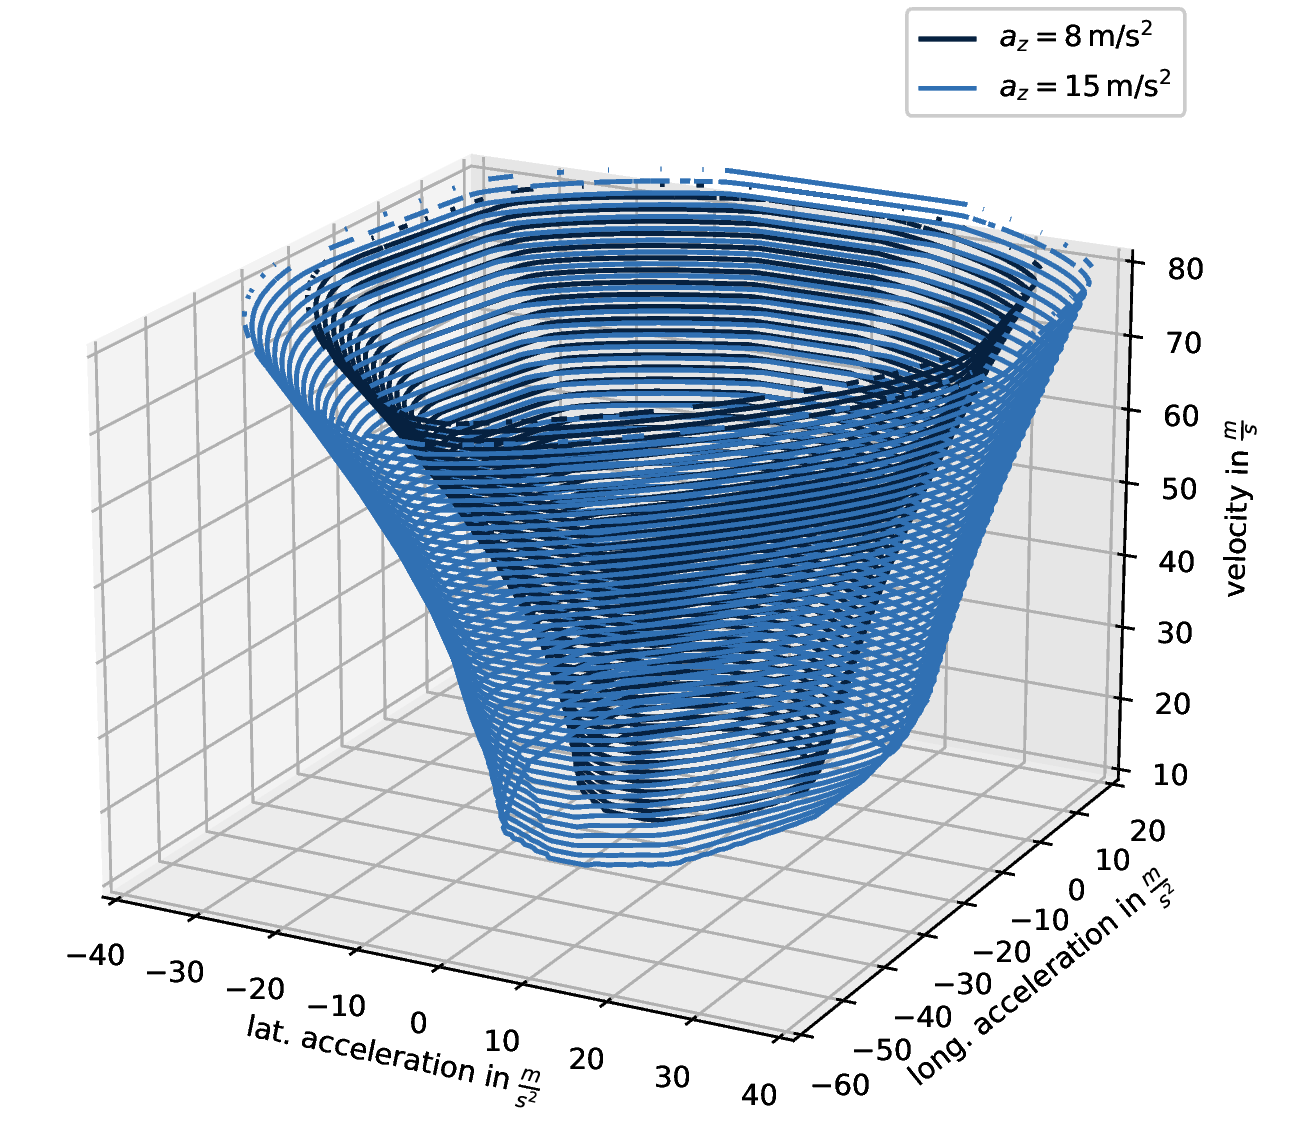
\includegraphics[width=0.6\textwidth]{figures/gggv_tornado.png}
    \end{center}
    \caption{Ενδεικτικό διάγραμμα επιδόσεων (\textit{GGV}) \cite{TUM_GGGVDiagrams}}
\label{fig:GGGV-Diagram-Sample}
\end{figure}

Στον αλγόριθμο προσομοίωσης γύρου, το προφίλ ταχύτητας $v(s)$ κατασκευάζεται με δύο διαδοχικές σαρώσεις κατά μήκος της
πίστας. Στην πρώτη, κατά τη φορά της πίστας, το όχημα επιταχύνεται σε κάθε σημείο με
το μέγιστο επιτρεπτό $a_x^+$, δίνοντας το προφίλ που περιορίζεται από την πρόσφυση κατά
την επιτάχυνση. Στη δεύτερη, με αντίστροφη φορά, το όχημα επιβραδύνει με το μέγιστο δυνατό
$|a_x^-|$, δίνοντας το προφίλ που περιορίζεται κατά την πέδηση προς την επόμενη στροφή.
Το τελικό $v(s)$ προκύπτει ως το κατά σημείο ελάχιστο των δύο σαρώσεων και ικανοποιεί
ταυτόχρονα το όριο πρόσφυσης στην κορυφή κάθε στροφής και την ικανότητα του οχήματος να
επιταχύνει και να επιβραδύνει εντός των ορίων του διαγράμματος \cite{Brayshaw2005}. Ο χρόνος
γύρου δίνεται τελικά από την ολοκλήρωση:

\begin{equation}
    T = \int_{0}^{L}\dfrac{ds}{v(s)}
    \label{eq:lapTimeIntegral}
\end{equation}

όπου $L$ το συνολικό μήκος της πίστας.\\[10pt]

Ο βασικός περιορισμός της προσέγγισης είναι ότι η τροχιά του οχήματος
θεωρείται δεδομένη, και ότι εξ ορισμού παραλείπονται μεταβατικά φαινόμενα με έντονη μη-μόνιμη
συμπεριφορά. Η σύγκριση με προσομοιωτές βέλτιστου ελέγχου καταγράφει μη-αμελητέες
αποκλίσεις υπέρ των μη-μόνιμων μεθόδων \cite{Perantoni2014}. Οι προσομοιωτές QSS ωστόσο, προτιμώνται λόγω του σημαντικά χαμηλότερου υπολογιστικού κόστους και τη δυνατότητα
άμεσης ενσωμάτωσης πρόσθετων μοντέλων -- όπως το θερμοδυναμικό μοντέλο ελαστικών της
παρούσας εργασίας -- μέσω κατάλληλης ενημέρωσης του διαγράμματος επιδόσεων GGV. Σημαντικότερα, η ανεξαρτησία τους από μοντέλο οδηγού τις καθιστά λιγότερο ευαίσθητες, αποτυπώνοντας μια ποσοτικοποίηση των μέγιστων επιδόσεων του οχήματος. 

\subsection{Δημιουργία διαγράμματος επιδόσεων - διάγραμμα GGV}
\label{subsec:ggv}

Το διάγραμμα επιδόσεων GGV κατασκευάζεται εξ ολοκλήρου από το μοντέλο οχήματος-ελαστικών
που αναπτύχθηκε στα προηγούμενα κεφάλαια, αναζητώντας για κάθε συνδυασμό ταχύτητας $v$ και
διαμήκους επιτάχυνσης $a_x$ τη μέγιστη εγκάρσια επιτάχυνση $a_y$ που μπορεί να αναπτύξει
το όχημα εντός των ορίων πρόσφυσης των ελαστικών. Η διαδικασία δομείται σε τρία διαδοχικά
βήματα: (i) εύρεση των διαμήκων ορίων επιτάχυνσης-πέδησης σε ευθεία, (ii) διακριτοποίηση
του $a_x$ σε πλέγμα και (iii) αριθμητική επίλυση μοντέλου δύο βαθμών ελευθερίας για κάθε
σημείο του πλέγματος.\\[10pt]

% ----- TikZ: high-level GGV pipeline (hybrid ODE + warm-sweep) -----
\begin{figure}[htbp]
\centering
\begin{tikzpicture}[
    node distance=0.55cm and 1.0cm,
    block/.style   ={rectangle, draw=black, fill=white,      text width=7.0cm,
                     align=center, rounded corners=4pt, minimum height=0.95cm, font=\small},
    io/.style      ={rectangle, draw=black, fill=black!5,    text width=7.0cm,
                     align=center, rounded corners=2pt, minimum height=0.9cm, font=\small},
    outbox/.style  ={rectangle, draw=black, fill=black!12,   text width=7.0cm,
                     align=center, rounded corners=2pt, minimum height=0.9cm, font=\small\bfseries},
    decision/.style={diamond,   draw=black, fill=white,      text width=3.2cm,
                     align=center, font=\scriptsize, inner sep=1pt},
    arr/.style     ={->, thick, black}
]

  \node[io]                            (inp)    {Είσοδοι: παράμετροι οχήματος, \\
                                                  θερμοκρασία ελαστικών, ταχύτητες};

  \node[block, below=of inp]           (long)   {Για κάθε ταχύτητα: \\
                                                  εύρεση ορίων διαμήκους επιτάχυνσης};

  \node[block, below=of long]          (grid)   {Δημιουργία ομοιόμορφου πλέγματος \\
                                                  διαμήκους επιτάχυνσης};

  \node[block, below=of grid]          (ode)    {Ολοκλήρωση εξισώσεων κίνησης \\
                                                  με σταδιακή αύξηση γωνίας διεύθυνσης};

  \node[outbox, below=of ode]           (out)    {Έξοδος: γεωγραφικός τόπος GGV \\
                                                  για κάθε ταχύτητα, θετικά και αρνητικά όρια};

  \draw[arr] (inp)   -- (long);
  \draw[arr] (long)  -- (grid);
  \draw[arr] (grid)  -- (ode);
  \draw[arr] (ode)   -- (out);

\end{tikzpicture}
\caption{Διαδικασία δημιουργίας διαγράμματος GGV.}
\label{fig:ggv_flow}
\end{figure}
% ----- τέλος flowchart -----

\subsubsection{Διαμήκη όρια σε ευθεία}

Για δεδομένη ταχύτητα $v$ και μηδενική εγκάρσια επιτάχυνση ($a_y = 0$, $\delta = 0$,
$\beta = 0$), τα όρια $[a_{x,\min},\ a_{x,\max}]$ προκύπτουν από δυαδική αναζήτηση επί
του $a_x$. Κριτήριο τερματισμού αποτελεί το ολικό έλλειμμα πρόσφυσης, όπως ορίστηκε στην
\cref{eq:totalFxViolation}. Καθώς σε αυτή τη φάση δεν υπάρχει εγκάρσια δυναμική, το
πρόβλημα ανάγεται σε μονοδιάστατη αναζήτηση και επιλύεται πολύ γρήγορα, δίνοντας τα δύο
άκρα του πλέγματος διαμήκους επιτάχυνσης για κάθε ταχύτητα.\\[10pt]

Ξεκινώντας από αρχικό διάστημα $[a_{lo}^{(0)},\ a_{hi}^{(0)}]$ που περιέχει με ασφάλεια
το ζητούμενο όριο, σε κάθε επανάληψη $k$ ενημερώνονται τα άκρα με βάση το πρόσημο του
ελλείμματος στο μέσο του διαστήματος:

\begin{equation}
    \begin{aligned}
        a_{mid}^{(k)} &= \tfrac{1}{2}\bigl(a_{lo}^{(k)} + a_{hi}^{(k)}\bigr) \\[3pt]
        \bigl[a_{lo}^{(k+1)},\ a_{hi}^{(k+1)}\bigr] &=
        \begin{dcases}
            \bigl[a_{mid}^{(k)},\ a_{hi}^{(k)}\bigr] &,\ g_1\bigl(a_{mid}^{(k)}; v\bigr) > 0 \\[6pt]
            \bigl[a_{lo}^{(k)},\ a_{mid}^{(k)}\bigr] &,\ g_1\bigl(a_{mid}^{(k)}; v\bigr) \leq 0
        \end{dcases}
    \end{aligned}
    \label{eq:ggvBinarySearch}
\end{equation}

\noindent
Η αναζήτηση τερματίζει όταν $a_{hi}^{(k)} - a_{lo}^{(k)} < \varepsilon$ και το ζητούμενο
όριο προκύπτει ως $a_{x,\max} = a_{lo}$. Για την πέδηση η διαδικασία εκτελείται με ανάλογο
τρόπο σε αρνητικές τιμές του $a_x$, δίνοντας το $a_{x,\min}$. Η ροή της μεθόδου
απεικονίζεται στο \cref{fig:binary_search_flow}.\\[10pt]

% ----- TikZ: binary search for longitudinal acceleration limits -----
\begin{figure}[htbp]
\centering
\begin{tikzpicture}[
    node distance=0.55cm and 0.8cm,
    block/.style   ={rectangle, draw=black, fill=white,      text width=5.2cm,
                     align=center, rounded corners=4pt, minimum height=0.9cm, font=\small},
    io/.style      ={rectangle, draw=black, fill=black!5,    text width=5.2cm,
                     align=center, rounded corners=2pt, minimum height=0.9cm, font=\small},
    outbox/.style  ={rectangle, draw=black, fill=black!12,   text width=5.2cm,
                     align=center, rounded corners=2pt, minimum height=0.9cm, font=\small\bfseries},
    decision/.style={diamond,   draw=black, fill=white,      text width=2.4cm,
                     align=center, font=\scriptsize, inner sep=1pt},
    arr/.style     ={->, thick, black}
]

  \node[io]                          (inp)  {Είσοδος: ταχύτητα $v$, αρχικά όρια $[a_{lo},\ a_{hi}]$};
  \node[block, below=of inp]         (mid)  {$a_{mid} \leftarrow (a_{lo}+a_{hi})/2$};
  \node[block, below=of mid]         (viol) {Υπολογισμός ελλείμματος\\ πρόσφυσης $g_1(a_{mid}; v)$};
  \node[decision, below=of viol]     (feas) {$g_1 <= 0$;};
  \node[block, below=1.3cm of feas]  (upd)  {$a_{lo} \leftarrow a_{mid}$ (ναι) \\ $a_{hi} \leftarrow a_{mid}$ (όχι)};
  \node[decision, below=of upd]      (conv) {$a_{hi}-a_{lo} < \varepsilon$;};
  \node[outbox, below=of conv]       (out)  {Έξοδος: $a_{x,\max} = a_{lo}$ (ή $a_{x,\min}=a_{hi}$ για πέδηση)};

  \draw[arr] (inp)  -- (mid);
  \draw[arr] (mid)  -- (viol);
  \draw[arr] (viol) -- (feas);
  \draw[arr] (feas) -- (upd);
  \draw[arr] (upd)  -- (conv);
  \draw[arr] (conv) -- node[right, font=\scriptsize]{ναι} (out);

  % loop back to mid on "όχι"
  \draw[arr] (conv.east) -| ++(2.2cm,0) |- node[right, pos=0.25, font=\scriptsize]{όχι} (mid.east);

\end{tikzpicture}
\caption{Διάγραμμα ροής -- δυαδική αναζήτηση διαμήκους ορίου πρόσφυσης σε ευθεία.}
\label{fig:binary_search_flow}
\end{figure}
% ----- τέλος flowchart -----



\subsubsection{Διακριτοποίηση διαμήκους επιτάχυνσης}

Το διάστημα $[a_{x,\min},\ a_{x,\max}]$ διακριτοποιείται με συνημιτονική κατανομή, η
οποία συσσωρεύει περισσότερα σημεία κοντά στα δύο άκρα και αραιότερα στο μέσο. Η επιλογή
αυτή δικαιολογείται από τη μορφή του διαγράμματος (\ref{fig:GGGV-Diagram-Sample}): κοντά στα όρια επιτάχυνσης και πέδησης,
το εφικτό $a_y$ πέφτει απότομα προς το μηδέν, οπότε η αύξηση της πυκνότητας δείγματος
σε αυτές τις περιοχές βελτιώνει την ακρίβεια αναπαράστασης χωρίς να επιβαρύνει
δυσανάλογα το υπολογιστικό κόστος.\\[10pt]


\subsubsection{Επίλυση εγκάρσιας επιτάχυνσης}

Για κάθε ζευγάρι $(v,\ a_x)$ του πλέγματος, η μέγιστη εγκάρσια επιτάχυνση βρίσκεται μέσω
αριθμητικής ολοκλήρωσης ενός μοντέλου δύο βαθμών ελευθερίας (\cref{eq:vehicleMotion2,eq:vehicleMotion3}). Το διάνυσμα κατάστασης
είναι $\mathbf{x} = [U_y,\ \dot{\psi}]^T$, με $U_y$ την εγκάρσια συνιστώσα της ταχύτητας
στο πλαίσιο του οχήματος και $\dot{\psi}$ τον ρυθμό εκτροπής. Η γωνία διεύθυνσης
$\delta$ αυξάνει γραμμικά με τον χρόνο, $\delta(t) = \dot{\delta}_0\,t$, με ρυθμό
$\dot{\delta}_0 = \pm 0.2^\circ/\mathrm{s}$ και μέγιστο πλάτος $\pm 15^\circ$. Οι δύο
εξισώσεις κίνησης προκύπτουν από τα υπόλοιπα δυνάμεων-ροπής του τετράτροχου μοντέλου
(\cref{eq:stateSolverEquationSystem}):

\begin{equation}
    \begin{aligned}
        \dot{U}_y &= \dfrac{1}{M}\sum_{i=FL,\dots,RR} F_{y,i} \; - \; \dot{\psi}\,U_x \\[3pt]
        \ddot{\psi} &= \dfrac{1}{I_z}\sum_{i=FL,\dots,RR}\bigl(\vec{r}_i \times \vec{F}_i\bigr)_z
    \end{aligned}
    \label{eq:ggvOde}
\end{equation}

\noindent
όπου $M$ η μάζα του οχήματος και $I_z$ η ροπή αδράνειας ως προς τον κατακόρυφο άξονα του
κέντρου μάζας.
Οι εξισώσεις ολοκληρώνονται έως τη χρονική στιγμή που είτε η γωνία διεύθυνσης φτάσει το μέγιστο πλάτος, είτε
εμφανιστεί απόκλιση της λύσης (υπερστροφική αστάθεια). Το συμβάν αστάθειας σηματοδοτείται από υπερβολικές τιμές επιτάχυνσης εκτροπής $\ddot{\psi}$.
Από την τροχιά της λύσης επιλέγεται το σημείο με το μεγαλύτερο μέτρο εγκάρσιας
επιτάχυνσης $a_y = U_x\,\dot{\psi}$.
Εξ'ορισμού της επίλυσης, τα ελαστικά θα είναι πάντοτε ικανά να αποδώσουν το ζητούμενο φορτίο καθώς βρίσκονται εντός των ορίων $[a_{x,min}, a_{x,max}]$. Σημειώνεται πως οι αδράνειες $M,\ I_z$ επηρεάζουν αποκλειστικά τη μεταβατική κατάσταση και όχι τις μέγιστες επιταχύνσεις του οχήματος. Γι' αυτό τον λόγο, τίθενται σε αρκετά υψηλές τιμές στις εξισώσεις (\ref{eq:ggvOde}) ώστε να επιβραδύνουν την απόκριση, διευκολύνοντας έτσι τον επιλύτη να αναγνωρίσει τη στιγμή που επέρχεται αστάθεια.\\[10pt]

\begin{figure}[ht!]
    \begin{center}
        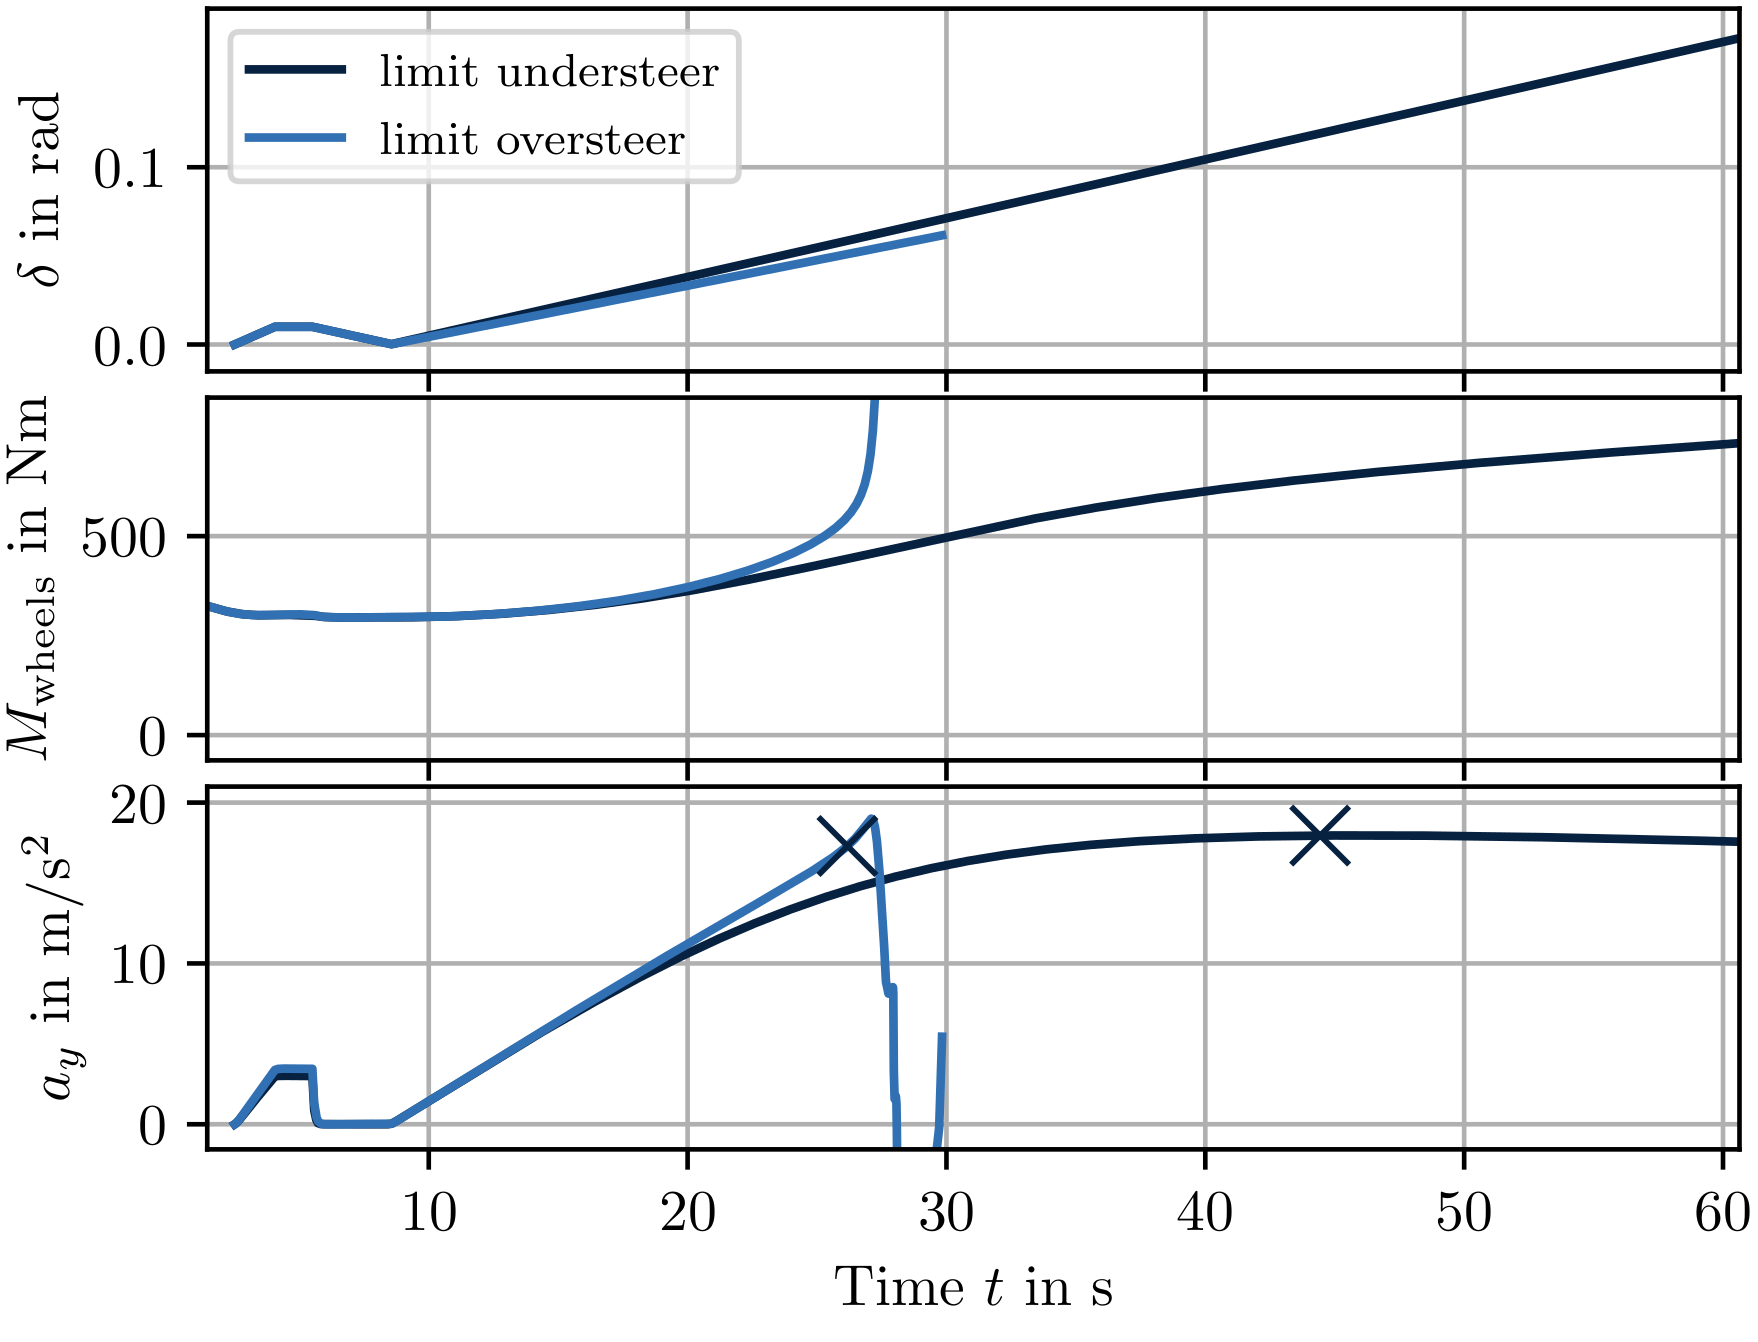
\includegraphics[width=0.6\textwidth]{figures/steering_ramp.png}
    \end{center}
    \caption{Μέθοδος εύρεσης μέγιστης πλευρικής επιτάχυνσης \cite{TUM_GGGVDiagrams}}
\label{fig:GGGV-Steering-Ramp}
\end{figure}

Η παραπάνω επίλυση εκτελείται δύο φορές ανά ζευγάρι $(v,\ a_x)$, με θετική και αρνητική
φορά της ράμπας γωνίας διεύθυνσης, δίνοντας ανεξάρτητα το θετικό και το αρνητικό άκρο
$a_{y,\max}$ και $a_{y,\min}$. Η ανεξάρτητη επίλυση των δύο πλευρών επιτρέπει στο
διάγραμμα να αποτυπώσει ασυμμετρίες που προκύπτουν από την ασύμμετρη κατάσταση των
ελαστικών, δηλαδή, διαφορετική θερμοκρασία και φθορά μεταξύ αριστερής και δεξιάς πλευράς.\\[10pt]



\subsubsection{Ενσωμάτωση ορίου κινητήρα}

Το διάγραμμα που προκύπτει από την παραπάνω διαδικασία αποτυπώνει αποκλειστικά τα όρια
πρόσφυσης του οχήματος και είναι ανεξάρτητο του ορίου ισχύος του κινητήρα. Ο περιορισμός
ισχύος εισάγεται στη συνέχεια, κατά τη διάρκεια της προσομοίωσης γύρου, ως πρόσθετος
έλεγχος: σε κάθε σημείο της πίστας, η τελικά διαθέσιμη διαμήκης επιτάχυνση προκύπτει από
το ελάχιστο μεταξύ της τιμής που υπαγορεύει το διάγραμμα και της τιμής που επιτρέπει η
καμπύλη δύναμης πρόωσης του κινητήρα στη δεδομένη ταχύτητα. Ο διαχωρισμός αυτός επιτρέπει
τον υπολογισμό του διαγράμματος μία μόνο φορά ανά κατάσταση ελαστικών. Επιπλέον, το \textit{GGV} είναι ένα πολύ ομαλό διάγραμμα, το οποίο δεν απαιτεί μεγάλο αριθμό κόμβων ταχύτητας για να αποτυπωθεί με ακρίβεια, ενώ η καμπύλη του κινητήρα θα απαιτούσε πολύ πυκνότερη διακριτοποίηση για την ακριβή αναπαράσταση των αλλαγών σχέσεων μετάδοσης κ.λπ.\\[10pt]

\subsubsection{Διόρθωση για φθορά και θερμοκρασία}

Κάθε διάγραμμα κατασκευάζεται υπό συγκεκριμένη κατάσταση θερμοκρασίας των ελαστικών, η
οποία υπεισέρχεται στον υπολογισμό μέσω του συντελεστή μείωσης πρόσφυσης
$\lambda(T)$ που παρουσιάστηκε στο \cref{sec:tyre_model}. Για τη σύνδεση με τον προσομοιωτή γύρου
κατασκευάζεται μια οικογένεια διαγραμμάτων σε διαφορετικές θερμοκρασίες αναφοράς, και το
τελικά χρησιμοποιούμενο διάγραμμα προκύπτει από παρεμβολή. Έτσι, η θερμική εξέλιξη των
ελαστικών κατά τη διάρκεια του γύρου αντικατοπτρίζεται σε ένα χρονο-μεταβαλλόμενο διάγραμμα
επιδόσεων, το οποίο μεταφέρει την επίδραση του θερμοδυναμικού μοντέλου στην τελική
εκτίμηση του χρόνου γύρου.\\
\noindent
Τα διαγράμματα αναφοράς δημιουργούνται για τις παρακάτω θερμοκρασίες.\\
\begin{equation*}
   T \in \{20, 40, 60, 80, 100, 120, 140\}\,^\circ\mathrm{C}
\end{equation*}

Για τον περιορισμό του πλήθους διαγραμμάτων αναφοράς που απαιτούνται, λαμβάνονται οι εξής παραδοχές.\\[6pt]
Αρχικά, σε κάθε κατάσταση, αγνοείται η ασυμμετρία των θερμοκρασιών -- υπολογίζεται η μέση θερμοκρασία των τεσσάρων ελαστικών, και υπολογίζεται το διάγραμμα επιδόσεων για αυτή τη θερμοκρασία. Στο \cref{fig:assymetricTemperatureEffect} φαίνεται το ποσοστιαίο σφάλμα αυτής της προσέγγισης, σε σχέση με τον ακριβή υπολογισμό. Η διαφορά φαίνεται να είναι μικρότερη από την τάξη του 3\%, επομένως, θεωρείται αποδεκτή δεδομένης της μείωσης του πλήθους των διαγραμμάτων. Εναλλακτικά, η επίδραση των ασύμμετρων θερμοκρασιών, θα μπορούσε να υπεισέλθει με τη μορφή ευαισθησίας κάθε κόμβου, ωστόσο, για την παρούσα υλοποίηση θεωρείται επαρκής η απλοποίηση της κοινής θερμοκρασίας.

\begin{figure}[ht!]
    \begin{center}
        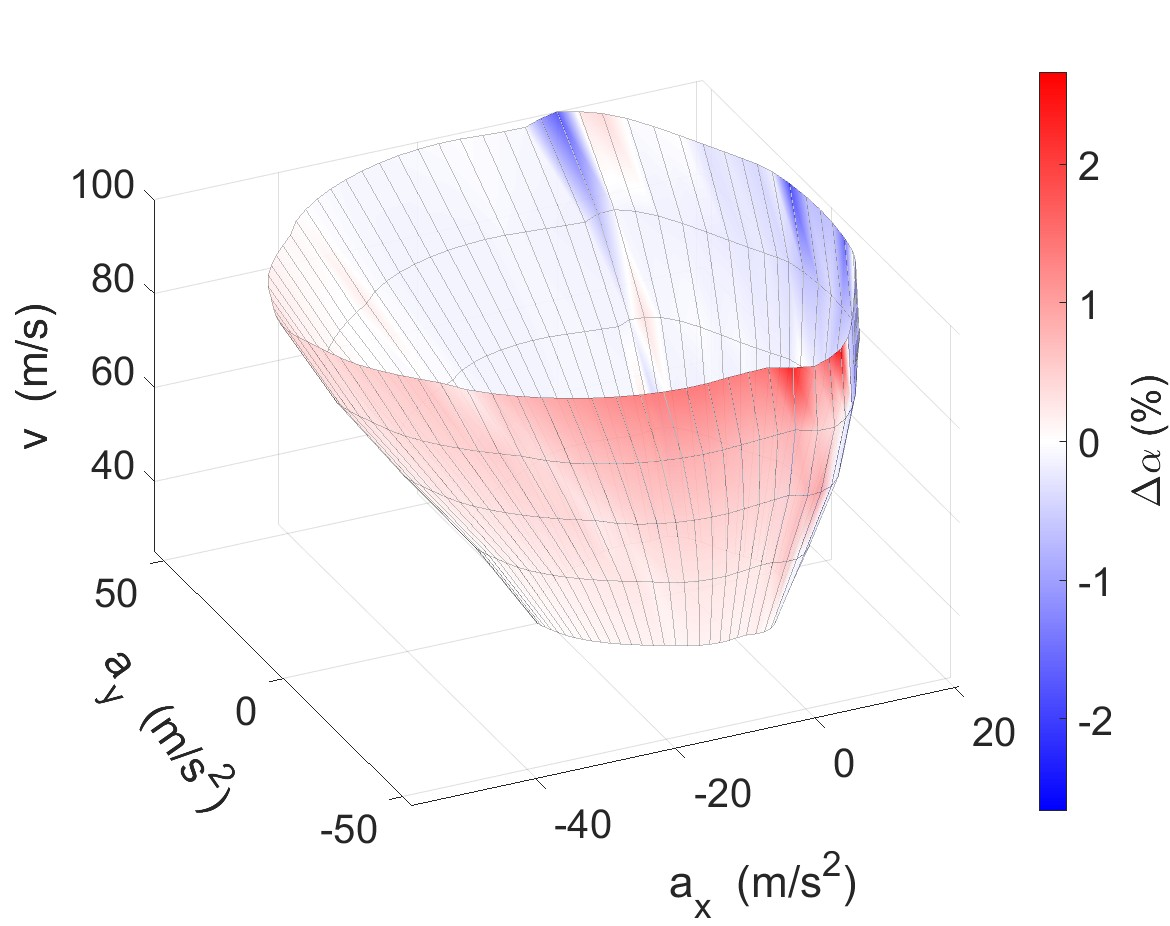
\includegraphics[width=0.6\textwidth]{figures/exact-vs-average-temperature.jpg}
    \end{center}
    \caption{Ποσοστιαίο σφάλμα προσέγγισης κοινής θερμοκρασίας - στις θετικές τιμές υπερεκτιμώνται οι επιδόσεις του οχήματος.}
\label{fig:assymetricTemperatureEffect}
\end{figure}

Επιπλέον, η φθορά συμπεριλαμβάνεται με τη χρήση του συντελεστή μείωσης (σχέση \ref{eq:wearScaleFactor}). Το διάγραμμα επιδόσεων δημιουργείται θεωρώντας μηδενική φθορά, και έπειτα όλα τα σημεία του διορθώνονται με τον συντελεστή μείωσης $\gamma(w_{max})$, της μέγιστης φθοράς, υπό τη θεώρηση πως το περισσότερο φθαρμένο ελαστικό κυριαρχεί στις επιδόσεις του οχήματος.

\subsubsection{Σχολιασμός διαγράμματος επιδόσεων}



Στο \cref{fig:2DGGV} φαίνεται η τυπική μορφή του διαγράμματος επιδόσεων. Η γενική μορφή είναι ανάλογη της αναμενόμενης, αποτελεί μία κλειστή καμπύλη σχεδόν ελλειπτικής μορφής.
Στα διαγράμματα του σχήματος \ref{fig:ggvProjections}, είναι εμφανής η επίδραση των αεροδυναμικών φορτίων. Καθώς αυξάνεται η ταχύτητα, αυξάνονται και οι μέγιστες επιταχύνσεις του οχήματος. Ωστόσο, δεν ακολουθούν αύξηση ανάλογη του τετραγώνου της ταχύτητας, λόγω του κορεσμού των ελαστικών, όπως περιγράφηκε στις \cref{eq:mu_load1,eq:mu_load2,eq:mu_load3,eq:mu_load}. Επιπλέον, γίνεται αντιληπτή και η επίδραση της οπισθέλκουσας: αφενός σε μεγαλύτερες ταχύτητες κυριαρχεί στη μέγιστη επιτάχυνση πέδησης, και αφετέρου στην περιοχή μέγιστης πρόωσης, αντισταθμίζει την επίδραση του κάθετου αεροδυναμικού φορτίου (αντίθετης άνωσης). Τελικά, σε ταχύτητα $100m/s$ η μέγιστη επιτάχυνση μειώνεται, όπου η μέγιστη διαμήκης δύναμη των κινητήριων τροχών δεν αυξάνεται αρκετά ώστε να υπερνικήσει την αύξηση της οπισθέλκουσας.

\begin{figure}[htbp!]
    \centering
    \begin{subfigure}[t]{0.48\textwidth}
        \centering
        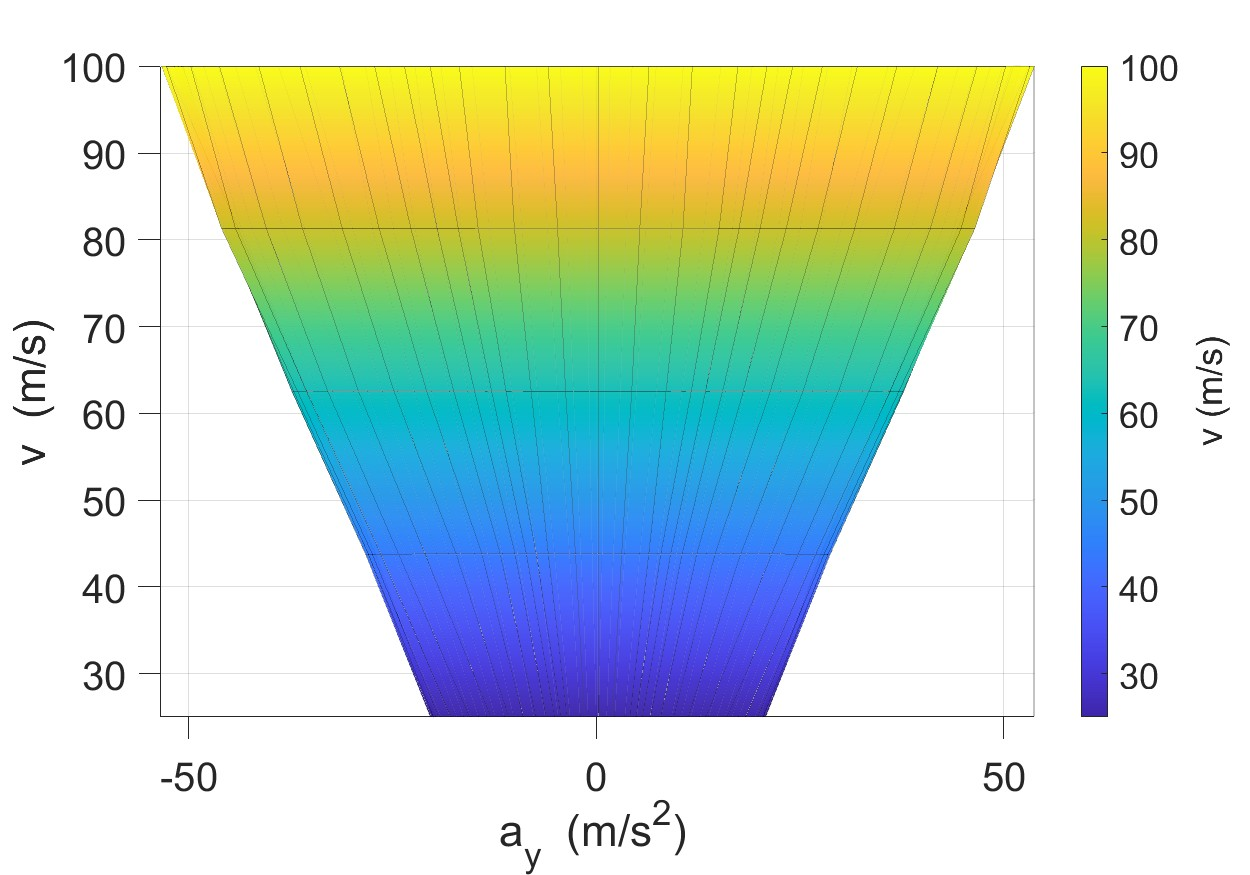
\includegraphics[width=\textwidth]{figures/ggv_front_view.jpg}
        \caption{Εμπρόσθια προβολή διαγράμματος επιδόσεων}
        \label{fig:ggvFrontView}
    \end{subfigure}
    \hfill
    \begin{subfigure}[t]{0.48\textwidth}
        \centering
        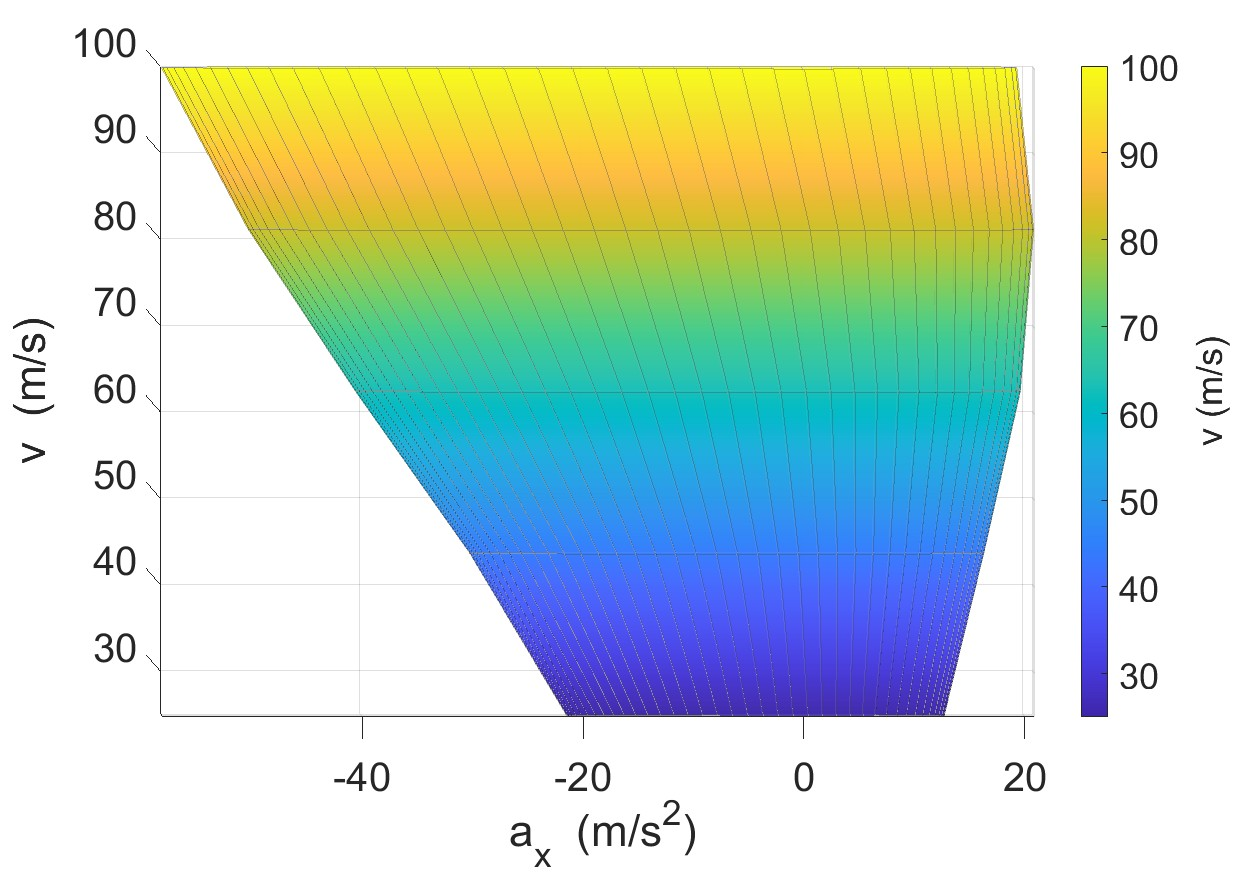
\includegraphics[width=\textwidth]{figures/ggv_side_view.jpg}
        \caption{Πλαϊνή προβολή διαγράμματος επιδόσεων}
        \label{fig:ggvSideView}
    \end{subfigure}
    \caption{Ενδεικτική μορφή διαγράμματος επιδόσεων σε προβολή σε δύο επίπεδα}
    \label{fig:ggvProjections}
\end{figure}

\FloatBarrier

Επίσης, μια σημαντική παρατήρηση είναι πως στην πλευρική επιτάχυνση παρατηρούνται σχεδόν δύο κορυφές -- η μία στην περιοχή επιβράδυνσης και μία στην περιοχή πρόωσης. Μελετώντας αρχικά τη μετακίνηση της κορυφής στην περιοχή επιβράδυνσης, παρατηρείται πως η μέγιστη πλευρική επιτάχυνση εμφανίζεται σε ολοένα και μεγαλύτερη επιβράδυνση καθώς αυξάνεται η ταχύτητα. Αυτό είναι φυσική απόρροια της κατασκευής του διαγράμματος καθώς συμπεριλαμβάνονται και τα αεροδυναμικά φορτία. Η μέγιστη πλευρική επιτάχυνση αναμένεται να εμφανιστεί στο σημείο όπου τα ελαστικά δεν παράγουν διαμήκες φορτίο, δηλαδή όταν δεν επιταχύνουν αλλά ούτε επιβραδύνουν. Καθώς αυξάνεται η ταχύτητα, η αεροδυναμική αντίσταση αυξάνεται με το τετράγωνό της, επομένως το όχημα επιβραδύνει παθητικά, χωρίς την ανάγκη για πέδηση, με αποτέλεσμα τη μεταφορά του σημείου μέγιστης πλευρικής επιτάχυνσης προς την περιοχή πέδησης.\\
\noindent
Στο όχημα του σχήματος \ref{fig:2DGGV}, ο κινητήριος άξονας είναι ο πίσω. Ως αποτέλεσμα, στην περιοχή πρόωσης, σε οριακές συνθήκες πρόσφυσης εμφανίζεται υπερστροφική συμπεριφορά (\textit{oversteer}), η οποία προκαλεί ένα ασταθές σημείο ισορροπίας (\cref{fig:GGGV-Steering-Ramp}). Επομένως, η κορυφή της περιοχής πρόωσης, αποτελεί τη μέγιστη πλευρική επιτάχυνση με υπερστροφικές συνθήκες, όπου απαιτείται διόρθωση του οδηγού για τη διατήρηση του ελέγχου του οχήματος.\\[6pt]

\noindent

\begin{figure}[hbpt!]
    \begin{center}
        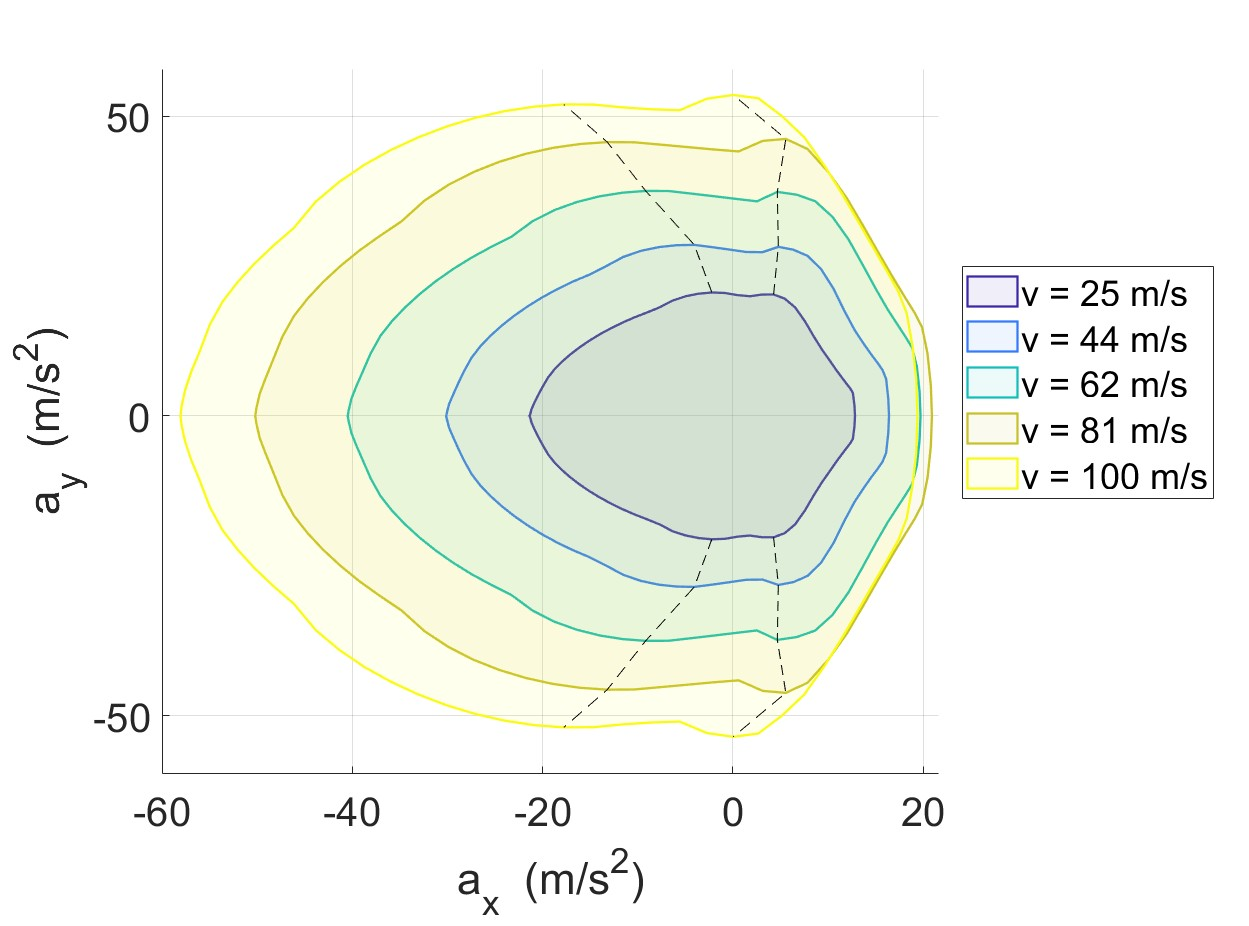
\includegraphics[width=0.75\textwidth]{figures/2DGGV_all80s.jpg}
    \end{center}
    \caption{Μορφή διαγράμματος επιδόσεων σε διαφορετικές ταχύτητες}
\label{fig:2DGGV}
\end{figure}

\FloatBarrier
\subsection{Ενσωμάτωση με προσομοιωτή γύρου - openLAP}
\label{subsec:openLAP}
Για την προσομοίωση γύρου, χρησιμοποιήθηκε το μοντέλο ανοιχτού κώδικα \openLap \cite{halkiopoulos_openlap_fileexchange,halkiopoulos_openlap_github} που περιλαμβάνει τον αλγόριθμο επίλυσης γύρου που περιγράφηκε στην εισαγωγή του κεφαλαίου \ref{sec:lapSim}.\\
\noindent
Οι μοναδικές επεμβάσεις που χρειάστηκαν στο \openLap ήταν οι εξής:

\paragraph{Ενσωμάτωση μοντέλου οχήματος.}
Καθώς το \openLap διαθέτει το δικό του μοντέλο οχήματος, όσοι υπολογισμοί αφορούν τη δυναμική του οχήματος, παρακάμφθηκαν, με την αντικατάστασή τους από την άμεση αναφορά στο διάγραμμα επιδόσεων του μοντέλου της παρούσας εργασίας. Συγκεκριμένα:

\begin{itemize}
    \item Για δεδομένη επιτάχυνση $a_y$, εύρεση $a_{x}^-,\ a_{x}^+$ μέσω διαγράμματος \textit{GGV}.
    \item Αφαίρεση επίδρασης οπισθέλκουσας -- το \openLap χρησιμοποιεί απλοποιημένο μοντέλο οχήματος σημειακής μάζας, το \text{GGV} του μοντέλου της εργασίας συμπεριλαμβάνει φαινόμενα της γεωμετρίας οχήματος και την επίδραση των αντιστάσεων.
\end{itemize}

\paragraph{Επίδραση θερμοκρασίας και φθοράς.}
Ένας επιλύτης \textit{QSS} δε διαθέτει την ιστορία του οχήματος κατά την επίλυση, δηλαδή, κάθε σημείο της πίστας αποτελεί ξεχωριστή κατάσταση και δεν επηρεάζεται από την προηγούμενη. Ένα πρακτικό αποτέλεσμα αυτής της παρατήρησης είναι πως κατά τον χρόνο της επίλυσης, δεν μπορεί να είναι γνωστή η εξέλιξη της θερμοκρασίας και της φθοράς.\\
\noindent
Επομένως, για να συμπεριληφθεί η επίδραση της κατάστασης του ελαστικού, χρησιμοποιείται μια (σχεδόν) επαναληπτική διαδικασία όπως περιγράφεται παρακάτω.

\begin{enumerate}
    \item Προσομοίωση ενός γύρου με σταθερές καταστάσεις ελαστικού κατά μήκος της πίστας (ίσες με τις αρχικές συνθήκες).
    \item Υπολογισμός εξέλιξης θερμοκρασίας και φθοράς, με τη μέθοδο του κεφαλαίου \ref{sec:inverseModel}.
    \label{bullet:tempReconstruction}
    \item Επανάληψη προσομοίωσης γύρου με τις καταστάσεις ελαστικού κατά μήκος της πίστας του βήματος \ref{bullet:tempReconstruction}.
\end{enumerate}

Τα βήματα \ref{bullet:tempReconstruction} και 3 θα μπορούσαν να επαναληφθούν έως να επέλθει σύγκλιση, ωστόσο, προς αποφυγή περιττών υπολογιστικών κύκλων, θεωρείται πως μια επανάληψη είναι αρκετή ώστε να αποτυπώσει την επίδραση της κατάστασης των ελαστικών στον χρόνο ενός γύρου (\cref{fig:iterT_tempPerTyre,fig:iterT_velocity}). Παρακάτω φαίνεται η σύγκριση μεταξύ της εξέλιξης της θερμοκρασίας αλλά και του προφίλ της ταχύτητας στις δύο διαδοχικές προσομοιώσεις του γύρου.

\begin{figure}[htbp!]
    \centering
    \begin{subfigure}[t]{0.48\textwidth}
        \centering
        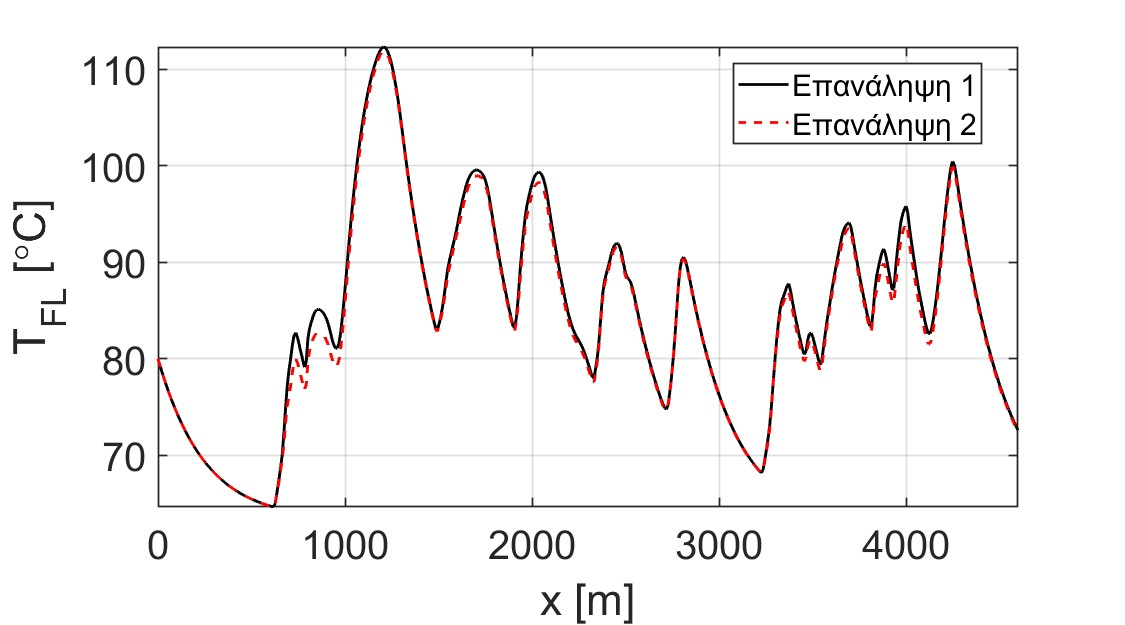
\includegraphics[width=\textwidth]{figures/iterativeT/T_convergence_FL.jpg}
    \end{subfigure}
    \hfill
    \begin{subfigure}[t]{0.48\textwidth}
        \centering
        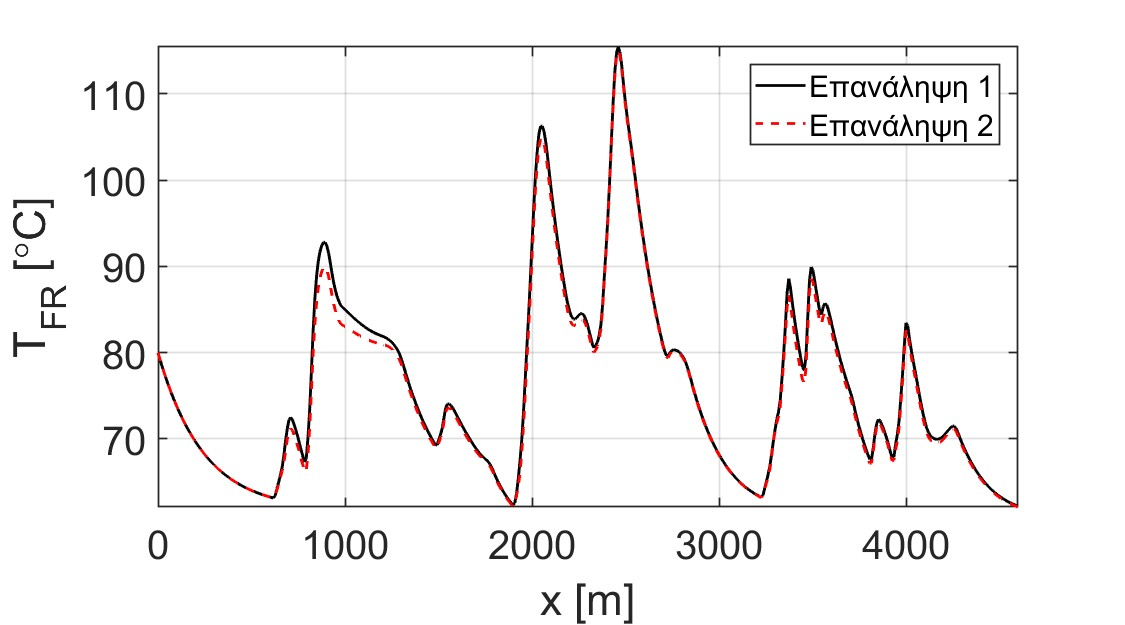
\includegraphics[width=\textwidth]{figures/iterativeT/T_convergence_FR.jpg}
    \end{subfigure}

    \vspace{0.5em}

    \begin{subfigure}[t]{0.48\textwidth}
        \centering
        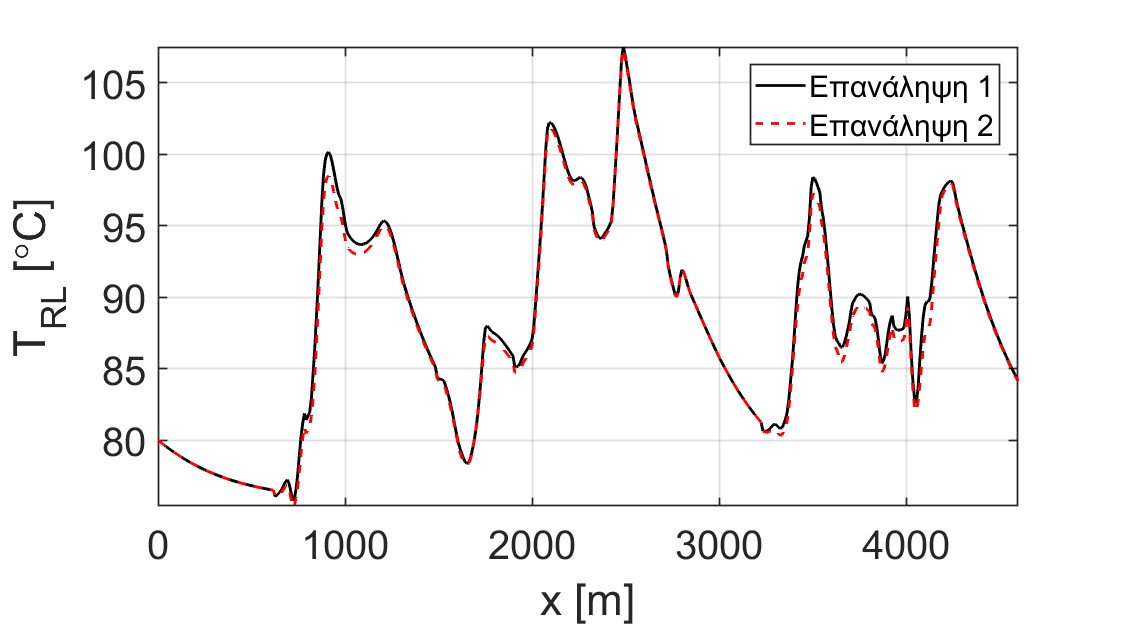
\includegraphics[width=\textwidth]{figures/iterativeT/T_convergence_RL.jpg}
    \end{subfigure}
    \hfill
    \begin{subfigure}[t]{0.48\textwidth}
        \centering
        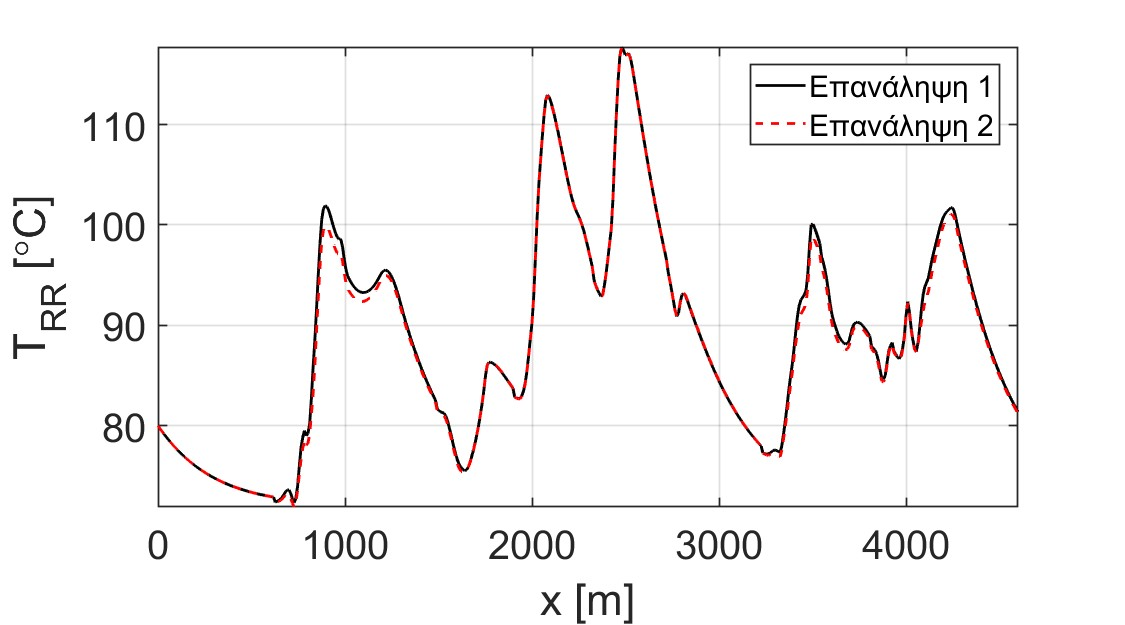
\includegraphics[width=\textwidth]{figures/iterativeT/T_convergence_RR.jpg}
    \end{subfigure}
    \caption{Σύγκριση $T_i(x)$ ανά ελαστικό ανάμεσα στην πρώτη (σταθερές συνθήκες) και στη δεύτερη επανάληψη (μεταβαλλόμενες συνθήκες).}
    \label{fig:iterT_tempPerTyre}
\end{figure}

\begin{figure}[htbp!]
    \centering
    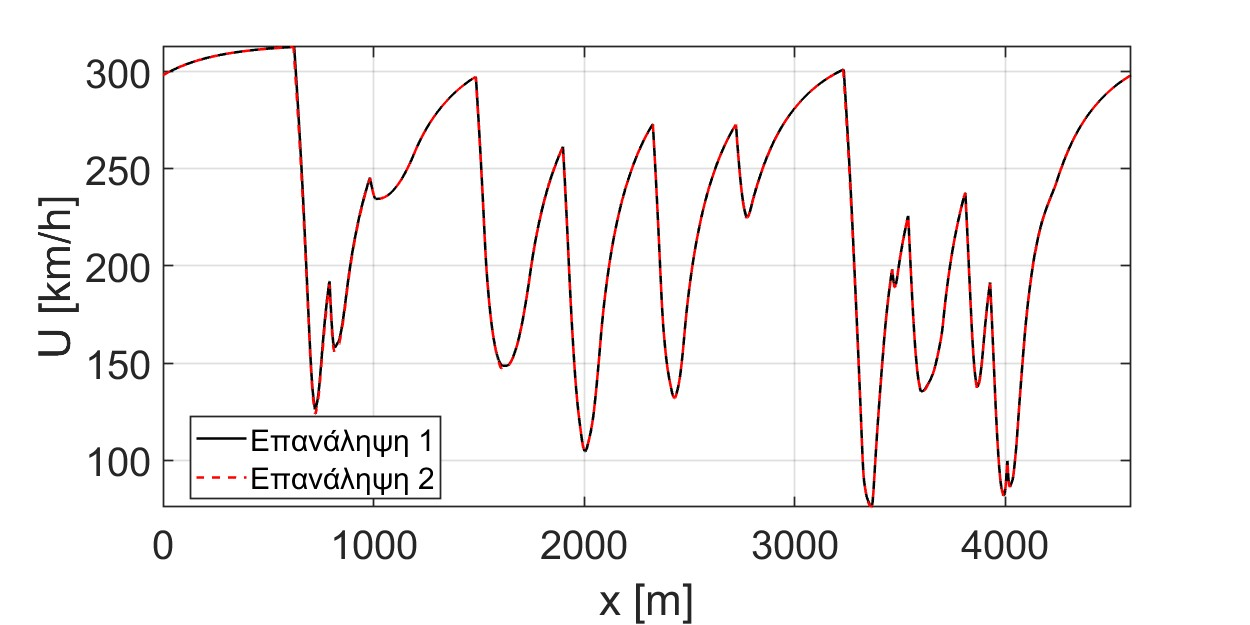
\includegraphics[width=0.85\textwidth]{figures/iterativeT/vel_iter.jpg}
    \caption{Προφίλ ταχύτητας $U(x)$ για τις δύο διαδοχικές επαναλήψεις.}
    \label{fig:iterT_velocity}
\end{figure}

\FloatBarrier



\clearoddpage
\section{Αποτελέσματα}
\label{sec:results}
\subsection{Δεδομένα οχήματος και πίστας}
Στο παρόν κεφάλαιο παρουσιάζονται τα αποτελέσματα σε επί μέρους μελέτες χρησιμοποιώντας τα μοντέλα που παρουσιάστηκαν στα προηγούμενα κεφάλαια. Η μελέτη βασίστηκε σε ένα όχημα τύπου \textit{Formula 1}, στην πίστα \textit{Circuit
de Barcelona-Catalunya}. Οι παράμετροι του οχήματος παρουσιάζονται στους \cref{tab:params_vehicle,tab:params_transmission}, και η καμπύλη του κινητήρα στο \cref{fig:engine_curve}. Οι παράμετροι των ελαστικών και οι αρχικές τιμές του θερμοδυναμικού μοντέλου είναι αυτές που παρουσιάζονται στους πίνακες του κεφαλαίου \ref{sec:tyre_model}, και αντιστοιχούν σε ελαστικά μαλακής γόμας \cite{Tremlett2016}. Οι παράμετροι του οχήματος αντικατοπτρίζουν το όχημα αναφοράς των \textit{Tremlett \& Limebeer} \cite{Tremlett2016} για σκοπούς σύγκρισης.

\begin{table}[htbp]
    \centering
    \small
    \renewcommand{\arraystretch}{1.2}
    \begin{tabular}{@{}l l l@{}}
        \toprule
        \textbf{Παράμετρος} & \textbf{Τιμή (Μονάδα)} & \textbf{Περιγραφή} \\
        \midrule
        $M$          & $660$ kg               & Μάζα οχήματος \\
        $L$          & $3.4$ m                & Μεταξόνιο \\
        $WD$         & $0.47$                 & Λόγος κατανομής βάρους στον εμπρόσθιο άξονα \\
        $h$          & $0.3$ m                & Ύψος κέντρου μάζας από το έδαφος \\
        $t_f$        & $1.46$ m               & Μετατρόχιο εμπρός άξονα \\
        $t_r$        & $1.46$ m               & Μετατρόχιο πίσω άξονα \\
        $R$          & $0.33$ m               & Ακτίνα τροχού \\
        $k_{br,f}$   & $0.65$                 & Κατανομή πέδησης στον εμπρός άξονα \\
        $k_d$        & $5$ N·m/rpm & Συντελεστής στρεπτικής απόσβεσης διαφορικού \\
        $\rho$       & $1.2$ kg/m$^3$         & Πυκνότητα αέρα \\
        $A$          & $1.5$ m$^2$            & Επιφάνεια αναφοράς αεροδυναμικών φορτίων \\
        \bottomrule
    \end{tabular}
    \caption{Παράμετροι μοντέλου οχήματος.}
    \label{tab:params_vehicle}
\end{table}


\begin{table}[htbp]
    \centering
    \small
    \renewcommand{\arraystretch}{1.2}
    \begin{tabular}{@{}l l l@{}}
        \toprule
        \textbf{Παράμετρος} & \textbf{Τιμή} & \textbf{Περιγραφή} \\
        \midrule
        $\eta_{fg}$   & $0.92$   & Βαθμός απόδοσης τελικής μετάδοσης \\
        $\eta_{gb}$   & $0.98$   & Βαθμός απόδοσης κιβωτίου \\
        $i_{fg}$      & $7$      & Λόγος τελικής μετάδοσης \\
        $i_{g,1}$     & $2.57$   & Σχέση μετάδοσης $1^{\text{ης}}$ ταχύτητας \\
        $i_{g,2}$     & $2.11$   & Σχέση μετάδοσης $2^{\text{ης}}$ ταχύτητας \\
        $i_{g,3}$     & $1.75$   & Σχέση μετάδοσης $3^{\text{ης}}$ ταχύτητας \\
        $i_{g,4}$     & $1.46$   & Σχέση μετάδοσης $4^{\text{ης}}$ ταχύτητας \\
        $i_{g,5}$     & $1.29$   & Σχέση μετάδοσης $5^{\text{ης}}$ ταχύτητας \\
        $i_{g,6}$     & $1.13$   & Σχέση μετάδοσης $6^{\text{ης}}$ ταχύτητας \\
        $i_{g,7}$     & $1.00$   & Σχέση μετάδοσης $7^{\text{ης}}$ ταχύτητας \\
        \bottomrule
    \end{tabular}
    \caption{Παράμετροι συστήματος μετάδοσης.}
    \label{tab:params_transmission}
\end{table}

% ----- pgfplots: engine torque & power vs rpm -----
% Requires in main preamble:
%   \usepackage{pgfplots}
%   \pgfplotsset{compat=1.18}   % or newer
%
\begin{figure}[htbp]
\centering
\begin{tikzpicture}
    \begin{axis}[
        name=torqueAxis,
        width=0.85\textwidth,
        height=6.5cm,
        xlabel={Στροφές κινητήρα [rpm]},
        ylabel={Ροπή [Nm]},
        axis y line*=left,
        xmin=0, xmax=19000,
        ymin=0, ymax=450,
        xtick={0,2000,4000,6000,8000,10000,12000,14000,16000,18000},
        scaled x ticks=false,
        xticklabel style={/pgf/number format/1000 sep=\,},
        grid=both,
        grid style={dotted, gray!50},
        tick align=outside,
        legend style={
            at={(0.02,0.98)}, anchor=north west,
            draw=black!40, fill=white, fill opacity=0.9, text opacity=1,
            font=\small,
            row sep=1pt
        }
    ]
        \addplot+[
            color=blue!60!black,
            mark=*, mark size=1.8pt,
            thick,
            mark options={fill=blue!60!black, draw=blue!60!black}
        ] table[x index=0, y index=1] {figures/engine_curve.dat};
        \addlegendentry{Ροπή}

        % Phantom entry for the power series so both labels live in one legend
        \addlegendimage{
            color=red!60!black,
            mark=square*, mark size=1.6pt,
            thick, densely dashed,
            mark options={solid, fill=red!60!black, draw=red!60!black}
        }
        \addlegendentry{Ισχύς}
    \end{axis}

    \begin{axis}[
        width=0.85\textwidth,
        height=6.5cm,
        axis y line*=right,
        axis x line=none,
        ylabel={Ισχύς [kW]},
        xmin=0, xmax=19000,
        ymin=0, ymax=700,
    ]
        \addplot+[
            color=red!60!black,
            mark=square*, mark size=1.6pt,
            thick, densely dashed,
            mark options={solid, fill=red!60!black, draw=red!60!black}
        ] table[x index=0, y index=2] {figures/engine_curve.dat};
    \end{axis}
\end{tikzpicture}
\caption{Καμπύλη ροπής κινητήρα.}
\label{fig:engine_curve}
\end{figure}
% ----- τέλος engine curve -----


\FloatBarrier
\subsection{Βαθμονόμηση θερμοδυναμικού μοντέλου}
Σε αυτή την ανάλυση συγκρίνεται η υπολογισμένη θερμοκρασία που παράγει το μοντέλο της εργασίας έναντι των μετρημένων χρονοσειρών της θερμοκρασίας των \textit{Tremblett \& Limebeer} \cite{Tremlett2016} κατά την εξέλιξη ενός γύρου. Έπειτα, εφαρμόζεται η ρουτίνα του κεφαλαίου \ref{sec:parameterFitting} με σκοπό τη βελτιστοποίηση των παραμέτρων του θερμοδυναμικού μοντέλου προς βαθμονόμηση με πειραματικά δεδομένα.

\begin{figure}[htbp!]
    \centering
    \begin{subfigure}[t]{0.48\textwidth}
        \centering
        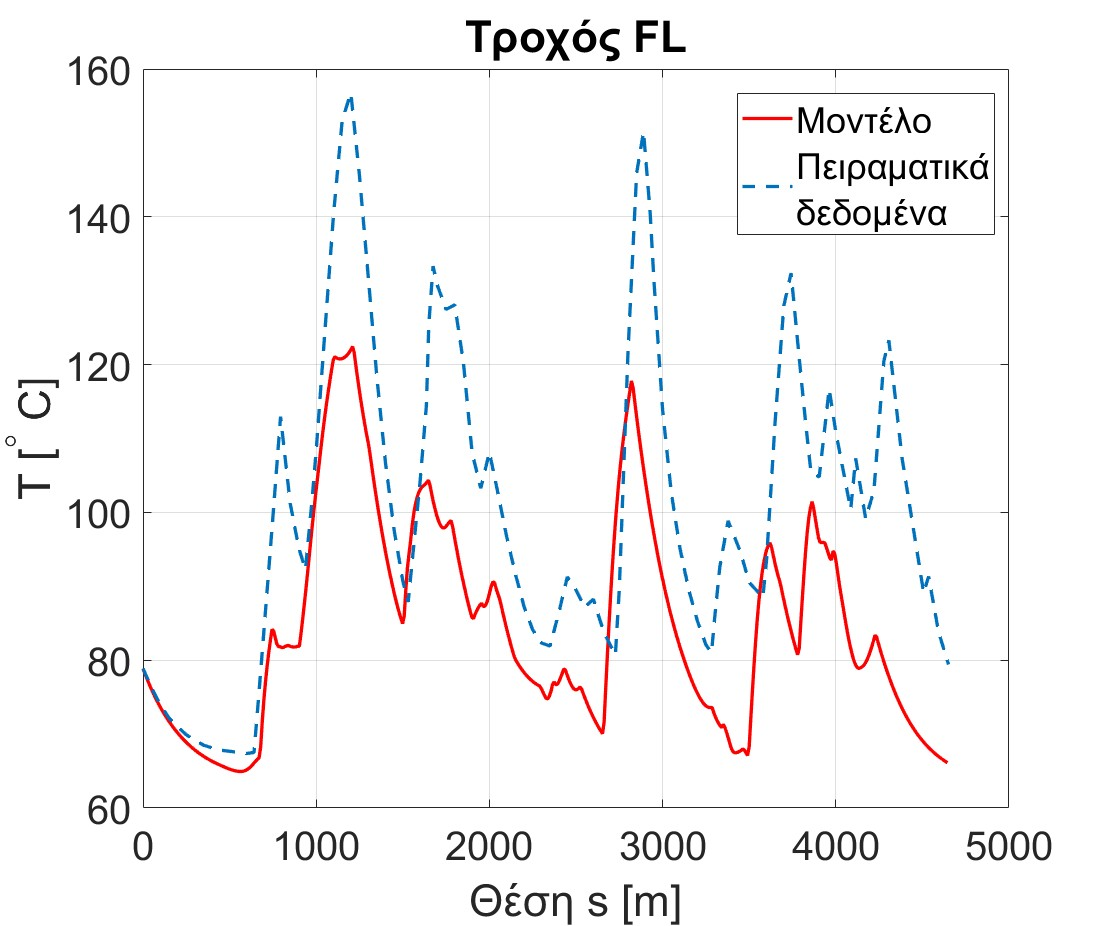
\includegraphics[width=\textwidth]{figures/FL_original_stateSolver_vs_Track.jpg}
    \end{subfigure}
    \hfill
    \begin{subfigure}[t]{0.48\textwidth}
        \centering
        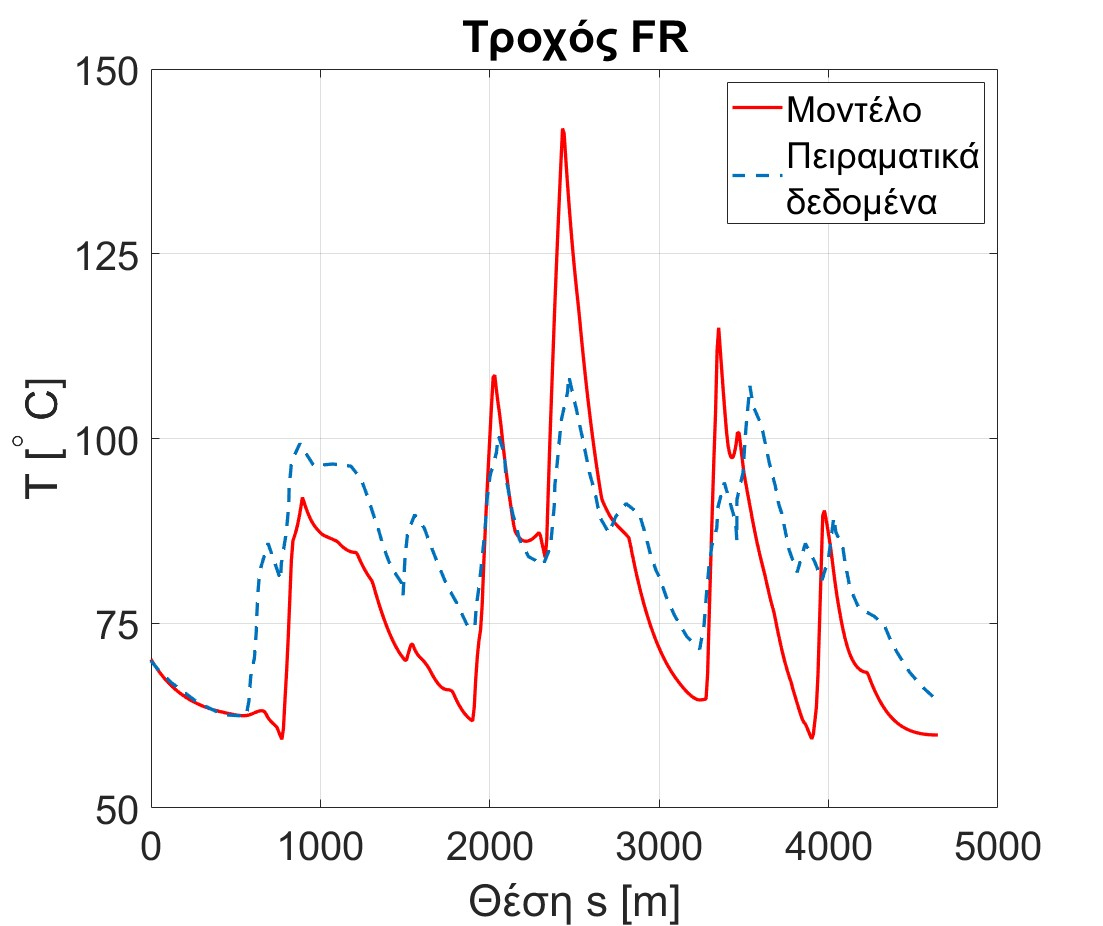
\includegraphics[width=\textwidth]{figures/FR_original_stateSolver_vs_Track.jpg}
    \end{subfigure}

    \vspace{0.5em}

    \begin{subfigure}[t]{0.48\textwidth}
        \centering
        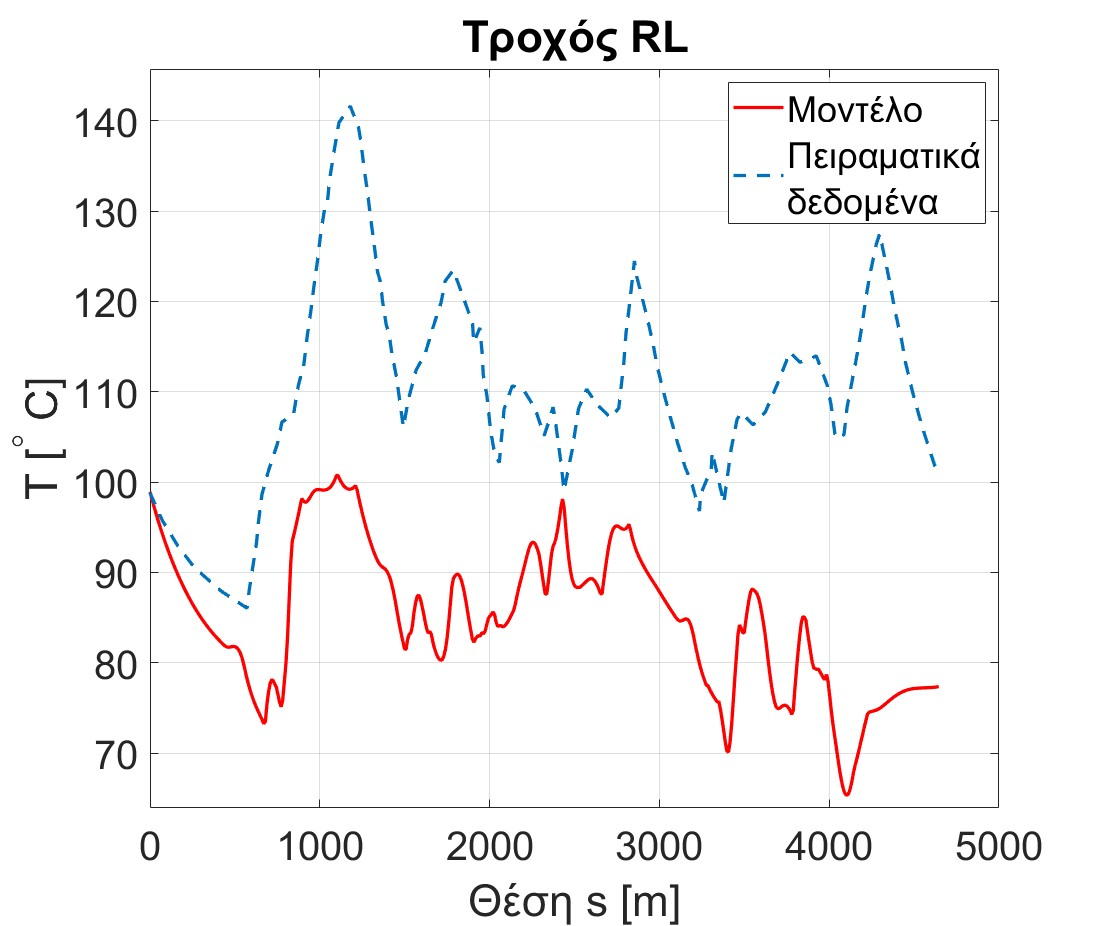
\includegraphics[width=\textwidth]{figures/RL_original_stateSolver_vs_Track.jpg}
    \end{subfigure}
    \hfill
    \begin{subfigure}[t]{0.48\textwidth}
        \centering
        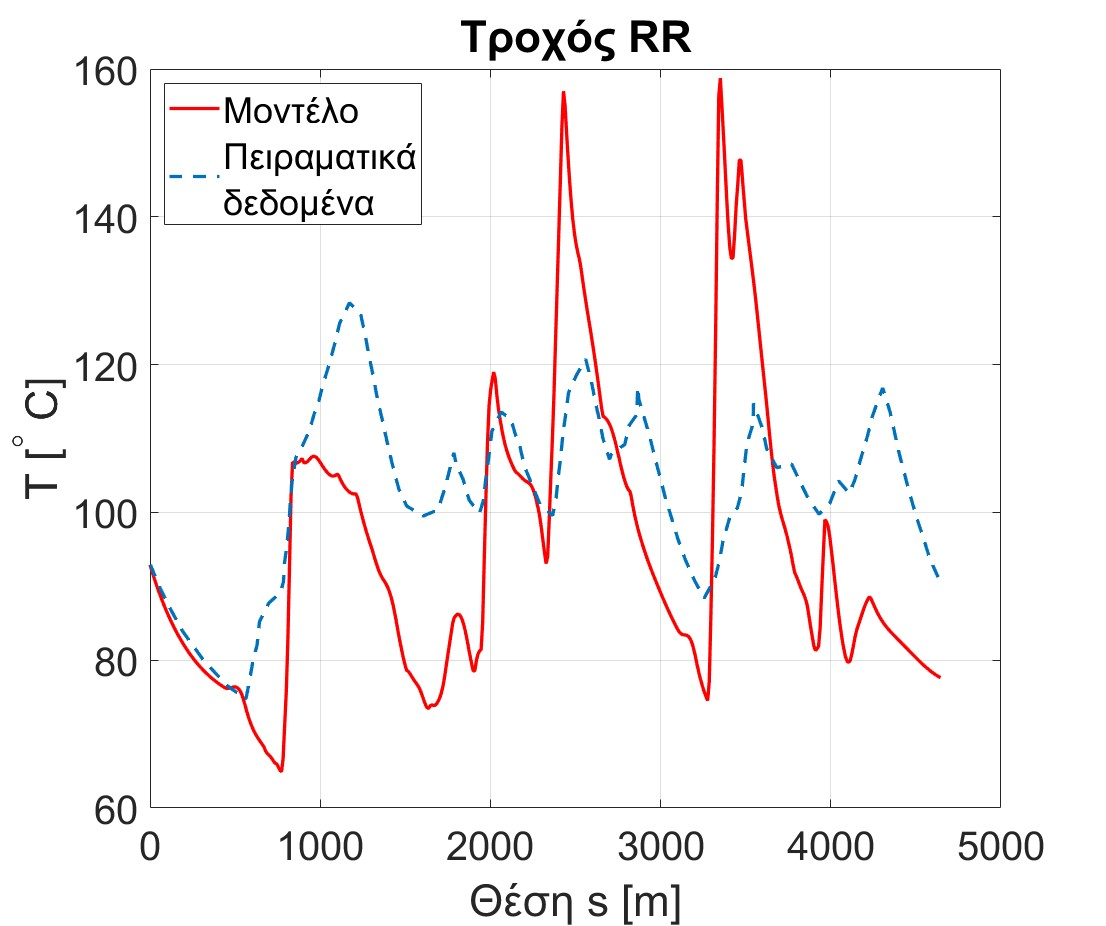
\includegraphics[width=\textwidth]{figures/RR_original_stateSolver_vs_Track.jpg}
    \end{subfigure}
    \caption{Σύγκριση θερμοκρασίας μοντέλου με πειραματική σε γύρο της πίστας \textit{Circuit de Barcelona - Catalunya}}
    \label{fig:defaultTemperaturesVsTests}
\end{figure}
%\label{sec:results}
%
%Σε αυτό το κεφάλαιο παρουσιάζονται τα αποτελέσματα της εφαρμογής της ολοκληρωμένης
%μεθοδολογίας: από την εκτίμηση μεγεθών ολίσθησης, μέσω της θερμικής προσομοίωσης, έως τη
%σύγκριση εναλλακτικών στρατηγικών οδήγησης. Η πίστα αναφοράς που χρησιμοποιήθηκε για όλες
%τις προσομοιώσεις είναι \textit{[TODO: αναφορά πίστας]}, με συνθήκες περιβάλλοντος $T_{\rm
%amb} = 25\,^\circ\mathrm{C}$ και $T_{\rm track} = 35\,^\circ\mathrm{C}$.
%
%% -------------------------
%\subsection{Εκτίμηση μεγεθών ολίσθησης}
%\label{subsec:results_slip}
%% -------------------------
%
%Η επεξεργασία του προφίλ ταχύτητας $v(s)$ και της γεωμετρίας πίστας $R(s)$ οδήγησε σε
%εκτίμηση των $\alpha_i$, $\kappa_i$ και $F_{z,i}$ για κάθε τροχό κατά μήκος πίστας. Ο
%αριθμός σημείων όπου ο solver δεν συνέκλινε ήταν \textit{[TODO: ποσοστό]}\%,
%συγκεντρωμένος κυρίως σε \textit{[TODO: περιοχές πίστας]}.
%
%% TODO: Σχήμα -- Εξέλιξη α_FL, α_FR, α_RL, α_RR κατά μήκος πίστας.
%% Επισήμανε τις κορυφές στις στροφές και τα μηδενικά στις ευθείες.
%%
%% \begin{figure}[htbp]
%%   \centering
%%   \includegraphics[width=\linewidth]{figures/slip_angles_vs_s.pdf}
%%   \caption{Γωνίες ολίσθησης τεσσάρων τροχών ως συνάρτηση θέσης πίστας.}
%%   \label{fig:slip_angles}
%% \end{figure}
%
%% TODO: Σχήμα -- Χάρτης converged/unconverged κατά μήκος πίστας.
%% Φωτίσε με χρώμα τα σημεία που δεν συνέκλινε ο solver.
%
%% -------------------------
%\subsection{Θερμική εξέλιξη ελαστικών}
%\label{subsec:results_thermal}
%% -------------------------
%
%Με τη χρήση των εκτιμημένων ολισθήσεων και του βαθμονομημένου θερμικού μοντέλου,
%υπολογίστηκε η εξέλιξη θερμοκρασίας $T(s)$ για κάθε τροχό. Τα αποτελέσματα αποκαλύπτουν
%σαφείς τάσεις ανάμεσα σε εμπρός/πίσω άξονα και εσωτερικό/εξωτερικό τροχό, συνδεόμενα άμεσα
%με τη μεταφορά φορτίου στις στροφές.
%
%% TODO: Σχήμα -- Θερμοκρασία 4 τροχών T(s) vs s.
%% Σήμανε το thermal window (T_tp±ΔT) με οριζόντιες ζώνες για οπτική αναφορά.
%%
%% \begin{figure}[htbp]
%%   \centering
%%   \includegraphics[width=\linewidth]{figures/temperature_evolution.pdf}
%%   \caption{Εξέλιξη θερμοκρασίας πέλματος (dT/ds ολοκλήρωση RK4) για τέσσερις τροχούς.
%%   Η ζώνη $T_{\rm tp}\pm 10\,^\circ\mathrm{C}$ σκιάζεται σε γκρι.}
%%   \label{fig:temp_evo}
%% \end{figure}
%
%% TODO: Σχήμα -- G-G plot με χρωματική κωδικοποίηση θερμοκρασίας.
%% Κάθε σημείο $(a_x, a_y)$ χρωματίζεται ανάλογα με T_FL (ή μέσο όρο).
%% Δείχνει εύγλωττα πότε εκμεταλλευόμαστε τα ελαστικά εντός/εκτός window.
%
%% -------------------------
%\subsection{Φθορά ελαστικών}
%\label{subsec:results_wear}
%% -------------------------
%
%Ο ρυθμός φθοράς $W_{\rm total}(s)$ αντικατοπτρίζει τη συνισταμένη και των τριών μηχανισμών
%(abrasion, graining, blistering). Σε συνθήκες hot-lap, ο κυρίαρχος μηχανισμός ήταν
%\textit{[TODO: συμπλήρωσε βάσει αποτελεσμάτων]}, με εξαίρεση \textit{[TODO: τμήματα πίστας
%ή φάσεις γύρου]}.
%
%% TODO: Σχήμα -- W_total(s) ανά τροχό. Επισήμανε κορυφές σε slow corners
%% (graining αν Τ<Τ_tp) ή μετά από μακριά straight (blistering αν Τ>Τ_tp).
%
%% -------------------------
%\subsection{Σύγκριση σεναρίων / παραμετρική ανάλυση}
%\label{subsec:results_parametric}
%% -------------------------
%
%Ο συνδυασμένος προσομοιωτής επιτρέπει παραμετρική ανάλυση δίχως φυσική δοκιμή. Εξετάστηκαν
%\textit{[TODO: αριθμός]} σενάρια που διαφέρουν ως προς \textit{[TODO: π.χ. πίεση
%ελαστικών, ρύθμιση ελατηρίων, αρχική θερμοκρασία, strategy]}:
%
%% TODO: Πίνακας ή σύνοψη σεναρίων -- παράμετροι που άλλαξαν και κύρια αποτελέσματα.
%% Παράδειγμα: lap time, μέσο T, ολικός ρυθμός φθοράς, χρόνος εκτός thermal window.
%
%% TODO: Σχήμα -- Σύγκριση θερμοκρασιακής εξέλιξης για διαφορετικά σενάρια
%% (π.χ. ψυχρή vs. θερμή εκκίνηση, ή διαφορετικά compounds).
%
%\subsection{Εξέλιξη θερμοκρασίας \& φθοράς σε αγώνα}
\clearoddpage
\section{Συμπεράσματα - βελτιώσεις}
\label{sec:conclusions}
Στην παρούσα εργασία αναπτύχθηκε ένα πλαίσιο προσομοίωσης χρόνου γύρου ψευδο-μόνιμης κατάστασης που
λαμβάνει υπόψη τη θερμοκρασία και τη φθορά των ελαστικών, συνδέοντας ένα θερμοδυναμικό μοντέλο ελαστικού
με τον προσομοιωτή \openLap μέσω ενός χρονο-μεταβαλλόμενου διαγράμματος επιδόσεων (\textit{GGV}).
Το τελικό μοντέλο έχει μία αρθρωτή (\textit{modular}) δομή, ώστε κάθε συνιστώσα του μοντέλου να μπορεί να αντικατασταθεί και να εμπλουτισθεί ανεξάρτητα, διατηρώντας τη συνολική λειτουργία του μοντέλου αναλλοίωτη.

\subsection{Χρησιμότητα του μοντέλου και κύρια ευρήματα}

Το κυριότερο αποτέλεσμα της εργασίας είναι πως η κατάσταση των ελαστικών μπορεί να ενσωματωθεί σε έναν
προσομοιωτή ψευδο-μόνιμης κατάστασης με απλό τρόπο, μέσω του διαγράμματος επιδόσεων, διατηρώντας τα
πλεονεκτήματα της προσέγγισης: χαμηλό υπολογιστικό κόστος και ανεξαρτησία από μοντέλο οδηγού. Η επίδραση
της θερμοκρασίας δεν είναι αμελητέα -- ο γύρος με ψυχρά ελαστικά ($30\,^\circ\mathrm{C}$) προέκυψε περίπου
$3\,\mathrm{s}$ πιο αργός από τον γύρο με θερμά ($90\,^\circ\mathrm{C}$), διαφορά που ένας κλασικός
προσομοιωτής με σταθερό διάγραμμα επιδόσεων δεν μπορεί να αποτυπώσει. Επιπλέον, φάνηκε πως μία μόνο
επανάληψη μεταξύ προσομοίωσης γύρου και υπολογισμού θερμοκρασίας είναι αρκετή, και πως η χρήση κοινής
μέσης θερμοκρασίας για τα τέσσερα ελαστικά εισάγει σφάλμα μικρότερο του $3\%$ στο διάγραμμα επιδόσεων.\\[8pt]
Η μέθοδος εκτίμησης κατάστασης είναι χρήσιμη και από μόνη της: με δεδομένα μόνο την ταχύτητα και την
τροχιά του οχήματος, δίνει τα μεγέθη ολίσθησης και τα φορτία κάθε τροχού, μεγέθη που στην πράξη είναι
ακριβό ή σχεδόν αδύνατο να μετρηθούν. Σε σύγκριση με τις μετρήσεις των \textit{Tremlett \& Limebeer}
\cite{Tremlett2016}, το μοντέλο αποτυπώνει ποιοτικά σωστά την εξέλιξη της θερμοκρασίας, με αύξηση και
μείωση στα ίδια σημεία της πίστας, ενώ η βαθμονόμηση μείωσε σημαντικά το σφάλμα RMS σε όλους τους
τροχούς (π.χ. στον τροχό \textit{RL} από $27.5$ σε $5.8\,^\circ\mathrm{C}\,\mathrm{RMS}$).\\[8pt]
Από την ανάλυση ευαισθησίας προκύπτει πως κυρίαρχη παράμετρος είναι ο εκθέτης ταχύτητας της συναγωγής
$p_6$ -- δηλαδή η ψύξη από τον αέρα στις ευθείες καθορίζει σε μεγάλο βαθμό τη θερμοκρασία του πέλματος --
ενώ το μοντέλο είναι σχεδόν ανεπηρέαστο από τις παραμέτρους $p_2, p_3$, γεγονός που υποδηλώνει πως το έργο
υστέρησης οφείλεται κυρίως στο κατακόρυφο φορτίο. Τέλος, ο ρυθμός φθοράς διαφοροποιείται έντονα κατά
μήκος της πίστας μεταξύ εμπρός/πίσω και εσωτερικού/εξωτερικού τροχού, ενώ η ευρετική συρρίκνωση του
διαγράμματος επιδόσεων με βάση τον ρυθμό φθοράς αποτελεί έναν πρώτο, απλό τρόπο προσέγγισης του
συμβιβασμού μεταξύ χρόνου γύρου και φθοράς, και αντικατοπτρίζει με ευκρίνεια την αλληλοεξάρτηση της κατάστασης των ελαστικών. Ακόμη και με τις απλοποιήσεις του, το μοντέλο είναι ικανό να ποσοτικοποιήσει μέσω της φυσικής του τους εμπειρικούς και διαισθητικούς κανόνες που έχουν θεμελιωθεί στον χώρο του μηχανοκίνητου αθλητισμού.

\subsection{Περιορισμοί}

Παρά τα παραπάνω, τα αποτελέσματα πρέπει να ερμηνεύονται κυρίως ποιοτικά. Ο σημαντικότερος περιορισμός της παρούσας εργασίας
είναι η έλλειψη δεδομένων: η βαθμονόμηση βασίστηκε σε δεδομένα ενός μόνο γύρου από τη βιβλιογραφία,
χωρίς να είναι βέβαιη η εγκυρότητα των δεδομένων. Οι
βελτιστοποιημένες παράμετροι μεταβλήθηκαν πολύ και δεν κρίθηκαν αξιόπιστες, ενώ για τη φθορά δεν υπήρχαν
καθόλου μετρήσεις, επομένως το μοντέλο φθοράς δεν έχει επαληθευτεί.\\[8pt]
Στο θερμικό μοντέλο μοντελοποιήθηκε μόνο η θερμική μάζα του πέλματος. Χωρίς τον σκελετό του ελαστικού να
δρα ως «δεξαμενή» θερμότητας, η απόκριση είναι πολύ γρήγορη: τα ψυχρά ελαστικά φτάνουν σε μόνιμη
κατάσταση μέσα σε έναν μόνο γύρο, ενώ στην πραγματικότητα η προθέρμανση διαρκεί περισσότερο -- επομένως
η διαφορά των $3\,\mathrm{s}$ του ψυχρού γύρου είναι πιθανότατα υποεκτιμημένη. Επιπλέον, δε μοντελοποιήθηκε
η θερμότητα που μεταφέρεται από τα φρένα μέσω της ζάντας στο ελαστικό. Σε συνδυασμό με την ισχυρή ψύξη
από συναγωγή, οι θερμοκρασίες στο τέλος κάθε γύρου σταθεροποιήθηκαν σε χαμηλές τιμές (περίπου
$70$--$80\,^\circ\mathrm{C}$), ενώ εντός του γύρου σπάνια ξεπερνούν τους $100\,^\circ\mathrm{C}$. Συνδυαστικά με αυτό, δεν μοντελοποιήθηκε η παράμετρος της γωνίας \textit{toe}, θεωρώντας την μηδενική. Στην πραγματικότητα, η ρύθμιση της γωνίας αυτής αποτελεί κυρίαρχο μηχανισμό ελέγχου της θερμοκρασίας των ελαστικών και διατήρησής τους στο παράθυρο λειτουργίας (όπως π.χ. με τον δημοφιλή σχεδιασμό του \textit{DAS} από την \textit{Mercedes AMG F1 Team} \cite{WikipediaDualAxisSteering}).
Έτσι, το
ελαστικό λειτουργεί κυρίως κάτω από το θερμικό παράθυρο και η φθορά κυριαρχείται από το \textit{graining},
ενώ το \textit{blistering} ουσιαστικά δεν εμφανίζεται.\\[8pt]
Επίσης, αγνοούνται τα μεταβατικά
φαινόμενα στην είσοδο και έξοδο των στροφών και οι συνθήκες περιβάλλοντος θεωρούνται σταθερές. Τέλος, ως
προσομοιωτής ψευδο-μόνιμης κατάστασης, το μοντέλο εκτελεί κάθε γύρο στο όριο του διαγράμματος επιδόσεων,
οπότε η διαχείριση των ελαστικών από τον οδηγό αποτυπώνεται μόνο προσεγγιστικά.

\subsection{Μελλοντικές βελτιώσεις}

Η πιο άμεση βελτίωση είναι η βαθμονόμηση και επαλήθευση του μοντέλου με περισσότερα και συνεπή πειραματικά
δεδομένα: θερμοκρασίες από αισθητήρες υπερύθρων, και μετρήσεις πάχους πέλματος πριν και μετά από κάθε
σετ γύρων για τη φθορά. Στη μοντελοποίηση, η προσθήκη της θερμικής μάζας του σκελετού και της
θερμότητας των φρένων αναμένεται να διορθώσει τόσο τη χρονική απόκριση όσο και τη θερμοκρασία λειτουργίας
των ελαστικών. Επιπλέον, η μοντελοποίηση των γωνιών \textit{toe} και \textit{camber} θα επέτρεπε στους χρήστες του μοντέλου την εκ των προτέρων μελέτη του στησίματος (\textit{setup}) του οχήματος ξεχωριστά για κάθε πίστα με γνώμωνα τη διαχείριση θερμοκρασίας και φθοράς, οι οποίες όπως έχει γίνει ήδη αντιληπτό, κυριαρχούν στις επιδόσεις του οχήματος.
Σε ένα επόμενο βήμα, η αντικατάσταση της ευρετικής συρρίκνωσης του διαγράμματος
επιδόσεων από μια πραγματική βελτιστοποίηση στρατηγικής και τροχιάς θα αξιοποιούσε πλήρως τη δυνατότητα του πλαισίου
στον σχεδιασμό της στρατηγικής αγώνα. Το μοντέλο της παρούσας εργασίας δεν στοχεύει στην κάλυψη αυτής της ανάγκης, καθώς ήδη έχουν παρουσιασθεί στη βιβλιογραφία αντίστοιχες μελέτες (όπως π.χ. \cite{Tremlett2016}), ωστόσο το μοντέλο ψευδο-μόνιμης κατάστασης της παρούσας εργασίας, σε συνδυασμό με κατάλληλο αλγόριθμο βελτιστοποίησης, θα μπορούσε να αποτελέσει τη βάση μιας τέτοιας μελέτης.

\clearoddpage
\nocite{*}
\printbibliography[title={Βιβλιογραφία}]

